%  LaTeX support: latex@mdpi.com 
%DIF LATEXDIFF DIFFERENCE FILE
%DIF DEL round1_remote_sensing_Andrea_Gonzalez/remote_sensing_Andrea_Gonzalez.tex   Wed Jan  8 03:35:16 2025
%DIF ADD round2_remote_sensing_Andrea_Gonzalez/remote_sensing_Andrea_Gonzalez.tex   Wed Jan  8 03:35:16 2025
%  For support, please attach all files needed for compiling as well as the log file, and specify your operating system, LaTeX version, and LaTeX editor.

%=================================================================
\documentclass[journal,article,submit,pdftex,moreauthors]{Definitions/mdpi} 
\usepackage{mathrsfs}
\usepackage{makecell}
\usepackage{multicol}
\usepackage{subcaption}
\usepackage{caption}
%DIF 11a11
\usepackage{physics} %DIF > 
%DIF -------
\captionsetup[subfigure]{justification=centering}
\usepackage{float} %figure inside minipage


%--------------------
% Class Options:
%--------------------
%----------
% journal
%----------
% Choose between the following MDPI journals:
% acoustics, actuators, addictions, admsci, adolescents, aerobiology, aerospace, agriculture, agriengineering, agrochemicals, agronomy, ai, air, algorithms, allergies, alloys, analytica, analytics, anatomia, animals, antibiotics, antibodies, antioxidants, applbiosci, appliedchem, appliedmath, applmech, applmicrobiol, applnano, applsci, aquacj, architecture, arm, arthropoda, arts, asc, asi, astronomy, atmosphere, atoms, audiolres, automation, axioms, bacteria, batteries, bdcc, behavsci, beverages, biochem, bioengineering, biologics, biology, biomass, biomechanics, biomed, biomedicines, biomedinformatics, biomimetics, biomolecules, biophysica, biosensors, biotech, birds, bloods, blsf, brainsci, breath, buildings, businesses, cancers, carbon, cardiogenetics, catalysts, cells, ceramics, challenges, chemengineering, chemistry, chemosensors, chemproc, children, chips, cimb, civileng, cleantechnol, climate, clinpract, clockssleep, cmd, coasts, coatings, colloids, colorants, commodities, compounds, computation, computers, condensedmatter, conservation, constrmater, cosmetics, covid, crops, cryptography, crystals, csmf, ctn, curroncol, cyber, dairy, data, ddc, dentistry, dermato, dermatopathology, designs, devices, diabetology, diagnostics, dietetics, digital, disabilities, diseases, diversity, dna, drones, dynamics, earth, ebj, ecologies, econometrics, economies, education, ejihpe, electricity, electrochem, electronicmat, electronics, encyclopedia, endocrines, energies, eng, engproc, entomology, entropy, environments, environsciproc, epidemiologia, epigenomes, est, fermentation, fibers, fintech, fire, fishes, fluids, foods, forecasting, forensicsci, forests, foundations, fractalfract, fuels, future, futureinternet, futurepharmacol, futurephys, futuretransp, galaxies, games, gases, gastroent, gastrointestdisord, gels, genealogy, genes, geographies, geohazards, geomatics, geosciences, geotechnics, geriatrics, grasses, gucdd, hazardousmatters, healthcare, hearts, hemato, hematolrep, heritage, higheredu, highthroughput, histories, horticulturae, hospitals, humanities, humans, hydrobiology, hydrogen, hydrology, hygiene, idr, ijerph, ijfs, ijgi, ijms, ijns, ijpb, ijtm, ijtpp, ime, immuno, informatics, information, infrastructures, inorganics, insects, instruments, inventions, iot, j, jal, jcdd, jcm, jcp, jcs, jcto, jdb, jeta, jfb, jfmk, jimaging, jintelligence, jlpea, jmmp, jmp, jmse, jne, jnt, jof, joitmc, jor, journalmedia, jox, jpm, jrfm, jsan, jtaer, jvd, jzbg, kidneydial, kinasesphosphatases, knowledge, land, languages, laws, life, liquids, literature, livers, logics, logistics, lubricants, lymphatics, machines, macromol, magnetism, magnetochemistry, make, marinedrugs, materials, materproc, mathematics, mca, measurements, medicina, medicines, medsci, membranes, merits, metabolites, metals, meteorology, methane, metrology, micro, microarrays, microbiolres, micromachines, microorganisms, microplastics, minerals, mining, modelling, molbank, molecules, mps, msf, mti, muscles, nanoenergyadv, nanomanufacturing,\gdef\@continuouspages{yes}} nanomaterials, ncrna, ndt, network, neuroglia, neurolint, neurosci, nitrogen, notspecified, %%nri, nursrep, nutraceuticals, nutrients, obesities, oceans, ohbm, onco, %oncopathology, optics, oral, organics, organoids, osteology, oxygen, parasites, parasitologia, particles, pathogens, pathophysiology, pediatrrep, pharmaceuticals, pharmaceutics, pharmacoepidemiology,\gdef\@ISSN{2813-0618}\gdef\@continuous pharmacy, philosophies, photochem, photonics, phycology, physchem, physics, physiologia, plants, plasma, platforms, pollutants, polymers, polysaccharides, poultry, powders, preprints, proceedings, processes, prosthesis, proteomes, psf, psych, psychiatryint, psychoactives, publications, quantumrep, quaternary, qubs, radiation, reactions, receptors, recycling, regeneration, religions, remotesensing, reports, reprodmed, resources, rheumato, risks, robotics, ruminants, safety, sci, scipharm, sclerosis, seeds, sensors, separations, sexes, signals, sinusitis, skins, smartcities, sna, societies, socsci, software, soilsystems, solar, solids, spectroscj, sports, standards, stats, std, stresses, surfaces, surgeries, suschem, sustainability, symmetry, synbio, systems, targets, taxonomy, technologies, telecom, test, textiles, thalassrep, thermo, tomography, tourismhosp, toxics, toxins, transplantology, transportation, traumacare, traumas, tropicalmed, universe, urbansci, uro, vaccines, vehicles, venereology, vetsci, vibration, virtualworlds, viruses, vision, waste, water, wem, wevj, wind, women, world, youth, zoonoticdis 
% For posting an early version of this manuscript as a preprint, you may use "preprints" as the journal. Changing "submit" to "accept" before posting will remove line numbers.

%---------
% article
%---------
% The default type of manuscript is "article", but can be replaced by: 
% abstract, addendum, article, book, bookreview, briefreport, casereport, comment, commentary, communication, conferenceproceedings, correction, conferencereport, entry, expressionofconcern, extendedabstract, datadescriptor, editorial, essay, erratum, hypothesis, interestingimage, obituary, opinion, projectreport, reply, retraction, review, perspective, protocol, shortnote, studyprotocol, systematicreview, supfile, technicalnote, viewpoint, guidelines, registeredreport, tutorial
% supfile = supplementary materials

%----------
% submit
%----------
% The class option "submit" will be changed to "accept" by the Editorial Office when the paper is accepted. This will only make changes to the frontpage (e.g., the logo of the journal will get visible), the headings, and the copyright information. Also, line numbering will be removed. Journal info and pagination for accepted papers will also be assigned by the Editorial Office.

%------------------
% moreauthors
%------------------
% If there is only one author the class option oneauthor should be used. Otherwise use the class option moreauthors.

%---------
% pdftex
%---------
% The option pdftex is for use with pdfLaTeX. Remove "pdftex" for (1) compiling with LaTeX & dvi2pdf (if eps figures are used) or for (2) compiling with XeLaTeX.

%=================================================================
% MDPI internal commands - do not modify
\firstpage{1} 
\makeatletter 
\setcounter{page}{\@firstpage} 
\makeatother
\pubvolume{1}
\issuenum{1}
\articlenumber{0}
\pubyear{2023}
\copyrightyear{2023}
%\externaleditor{Academic Editor: Firstname Lastname}
\datereceived{ } 
\daterevised{ } % Comment out if no revised date
\dateaccepted{ } 
\datepublished{ } 
%\datecorrected{} % For corrected papers: "Corrected: XXX" date in the original paper.
%\dateretracted{} % For corrected papers: "Retracted: XXX" date in the original paper.
\hreflink{https://doi.org/} % If needed use \linebreak
%\doinum{}
%\pdfoutput=1 % Uncommented for upload to arXiv.org

%=================================================================
% Add packages and commands here. The following packages are loaded in our class file: fontenc, inputenc, calc, indentfirst, fancyhdr, graphicx, epstopdf, lastpage, ifthen, float, amsmath, amssymb, lineno, setspace, enumitem, mathpazo, booktabs, titlesec, etoolbox, tabto, xcolor, colortbl, soul, multirow, microtype, tikz, totcount, changepage, attrib, upgreek, array, tabularx, pbox, ragged2e, tocloft, marginnote, marginfix, enotez, amsthm, natbib, hyperref, cleveref, scrextend, url, geometry, newfloat, caption, draftwatermark, seqsplit
% cleveref: load \crefname definitions after \begin{document}

%=================================================================
% Please use the following mathematics environments: Theorem, Lemma, Corollary, Proposition, Characterization, Property, Problem, Example, ExamplesandDefinitions, Hypothesis, Remark, Definition, Notation, Assumption
%% For proofs, please use the proof environment (the amsthm package is loaded by the MDPI class).

%=================================================================
% Full title of the paper (Capitalized)
% \Title{Representation learning for crop type classification of multispectral multitemporal remote sensing data}
\Title{Representation learning of multispectral Earth Observation time series and evaluation for crop type classification}

% MDPI internal command: Title for citation in the left column
\TitleCitation{Title}

% Author Orchid ID: enter ID or remove command
\newcommand{\orcidauthorA}{0000-0001-9961-4763} % Add \orcidA{} behind the author's name
\newcommand{\orcidauthorB}{0000-0002-9813-7712} % Add \orcidB{} behind the author's name
\newcommand{\orcidauthorC}{0000-0003-2169-8009}
\newcommand{\orcidauthorD}{0000-0001-9703-3973}
% Authors, for the paper (add full first names)
\Author{Andrea González-Ramírez $^{1,*}$\orcidA{}, Clement Atzberger $^{2}$\orcidC{}, Deni Torres-Roman $^{1}$\orcidB{} and Josué López$^{2}$\orcidD{}}

%\longauthorlist{yes}

% MDPI internal command: Authors, for metadata in PDF
\AuthorNames{Firstname Lastname, Firstname Lastname and Firstname Lastname}

% MDPI internal command: Authors, for citation in the left column
\AuthorCitation{Lastname, F.; Lastname, F.; Lastname, F.}
% If this is a Chicago style journal: Lastname, Firstname, Firstname Lastname, and Firstname Lastname.

% Affiliations / Addresses (Add [1] after \address if there is only one affiliation.)
\address{%
$^{1}$ \quad Center for Research and Advanced Studies of the National 
Polytechnic Institute, Telecommunications Group, Av del Bosque 1145, 
Zapopan 45017, Mexico\\
% $^{2}$ \quad University of Natural Resources and Life Science, Institute of Geomatics, 
% Peter Jordan 82, Vienna 1180, Austria\\
$^{2}$ \quad Mantle Labs, Grünentorgasse 19, Vienna 1090, Austria}

% Contact information of the corresponding author
\corres{Correspondence: andrea.gonzalez@cinvestav.mx}%, deni.torres@cinvestav.mx and clement@mantle-labs.com}

% Current address and/or shared authorship
% \firstnote{Current address: Affiliation 3.} 
% \firstnote{These authors contributed equally to this work.}
% The commands \thirdnote{} till \eighthnote{} are available for further notes

%\simplesumm{} % Simple summary

%\conference{} % An extended version of a conference paper

% Abstract (Do not insert blank lines, i.e. \\) 
\abstract{Remote sensing (RS) spectral time series provide a substantial source of information for the regular and cost-efficient monitoring of the Earth surface.
Important monitoring tasks include land use and land cover classification, change detection, forest monitoring, crop type identification, among others.
To develop accurate solutions for RS-based applications, often supervised shallow/deep learning algorithms are used. 
%Recently, supervised deep learning algorithms are used to develop accurate solutions for applications involving RS data.
However, such approaches usually require fixed-length inputs and large labeled datasets.
% In addition, 
Unfortunately, RS images acquired by optical sensors are frequently degraded by aerosol contamination, clouds and cloud shadows, producing missing observations and irregular observation patterns.
To address these issues, efforts have been made to implement frameworks that generate meaningful representations from the irregularly sampled data streams and alleviate the deficiencies of the data sources and supervised algorithms.
Here, we propose a conceptually and computationally simple representation learning (RL) approach based on autoencoders (AEs) to generate discriminative features for crop type classification.
% using only a tiny set of reference samples.
% Our AEs architecture has very few parameters compared to other models proposed in the state-of-the-art, leading to a scalable model able to process very large areas in low computational time.
%\textcolor{orange}{Different to other papers, we propose a representation learning model based on autoencoders (AEs) to create informative and discriminative features for crop type classification.} In addition, \textcolor{orange}{the architecture is configured to keep very low number of parameters compared to other models proposed in the state of the art}, producing a scalable model able to process very large areas in low computational time.
The proposed methodology ensembles a set of single layer AEs with very limited number of neurons, each one trained with mono-temporal spectral features of a small set of samples belonging to a class, resulting in a model capable of processing very large areas in low computational time. Importantly, the developed approach remains flexible with respect to the availability of clear temporal observations.
% belonging to a specific crop type, with the aim of reducing reconstruction difference for samples from the same crop type. 
The signal derived from the ensemble of AE is the reconstruction difference vector between input samples and their corresponding estimations, which are averaged over all cloud/shadows-free temporal observations of a pixel location. This averaged reconstruction difference vector is the base for the representations and the subsequent classification. 
Experimental results show that the proposed extremely light-weight architecture indeed generates separable features for competitive performances in crop type classification, as distance metrics scores achieved with the derived representations significantly outperform those obtained with the initial data. Conventional classification models were trained and tested with representations generated from a widely used Sentinel-2 multispectral multitemporal dataset, BreizhCrops. 
%DIF 140c141
%DIF < Our method achieves $76.72\%$ overall accuracy which is $\sim 6\%$ higher than using original Sentinel-2 data within conventional classifiers and even $\sim 4\%$ better than complex deep models as OmnisCNN. Compared to extremely complex and time-consuming models such as transformers and LSTMs, only a $3\%$ reduction in overall accuracy was noted. Our method uses only $6.8k$ parameters, i.e., $\sim 400x$ less than OmnicsCNN and $\sim 27x$ less than Transformers. The results prove that our method is competitive in classification performance compared with state-of-the-art methods while requiring much lower computational load.}
%DIF -------
Our method achieves $77.06\%$ overall accuracy which is $\sim 6\%$ higher than using original Sentinel-2 data within conventional classifiers and even $\sim 4\%$ better than complex deep models as OmnisCNN. Compared to extremely complex and time-consuming models such as transformers and Long-short term memory (LSTM), only a $3\%$ reduction in overall accuracy was noted. Our method uses only $6.8k$ parameters, i.e., $\sim 400x$ less than OmnicsCNN and $\sim 27x$ less than Transformers. The results prove that our method is competitive in classification performance compared with state-of-the-art methods while substantially reducing the computational load.} %DIF > 
%DIF -------
% Keywords
\keyword{crop types; multispectral; multitemporal; autoencoder; representation learning} 

% The fields PACS, MSC, and JEL may be left empty or commented out if not applicable
%\PACS{J0101}
%\MSC{}
%\JEL{}

%%%%%%%%%%%%%%%%%%%%%%%%%%%%%%%%%%%%%%%%%%
% Only for the journal Diversity
%\LSID{\url{http://}}

%%%%%%%%%%%%%%%%%%%%%%%%%%%%%%%%%%%%%%%%%%
% Only for the journal Applied Sciences
%\featuredapplication{Authors are encouraged to provide a concise description of the specific application or a potential application of the work. This section is not mandatory.}
%%%%%%%%%%%%%%%%%%%%%%%%%%%%%%%%%%%%%%%%%%

%%%%%%%%%%%%%%%%%%%%%%%%%%%%%%%%%%%%%%%%%%
% Only for the journal Data
%\dataset{DOI number or link to the deposited data set if the data set is published separately. If the data set shall be published as a supplement to this paper, this field will be filled by the journal editors. In this case, please submit the data set as a supplement.}
%\datasetlicense{License under which the data set is made available (CC0, CC-BY, CC-BY-SA, CC-BY-NC, etc.)}

%%%%%%%%%%%%%%%%%%%%%%%%%%%%%%%%%%%%%%%%%%
% Only for the journal Toxins
%\keycontribution{The breakthroughs or highlights of the manuscript. Authors can write one or two sentences to describe the most important part of the paper.}

%%%%%%%%%%%%%%%%%%%%%%%%%%%%%%%%%%%%%%%%%%
% Only for the journal Encyclopedia
%\encyclopediadef{For entry manuscripts only: please provide a brief overview of the entry title instead of an abstract.}

%%%%%%%%%%%%%%%%%%%%%%%%%%%%%%%%%%%%%%%%%%
% Only for the journal Advances in Respiratory Medicine
%\addhighlights{yes}
%\renewcommand{\addhighlights}{%

%\noindent This is an obligatory section in “Advances in Respiratory Medicine”, whose goal is to increase the discoverability and readability of the article via search engines and other scholars. Highlights should not be a copy of the abstract, but a simple text allowing the reader to quickly and simplified find out what the article is about and what can be cited from it. Each of these parts should be devoted up to 2~bullet points.\vspace{3pt}\\
%\textbf{What are the main findings?}
% \begin{itemize}[labelsep=2.5mm,topsep=-3pt]
% \item First bullet.
% \item Second bullet.
% \end{itemize}\vspace{3pt}
%\textbf{What is the implication of the main finding?}
% \begin{itemize}[labelsep=2.5mm,topsep=-3pt]
% \item First bullet.
% \item Second bullet.
% \end{itemize}
%}

%%%%%%%%%%%%%%%%%%%%%%%%%%%%%%%%%%%%%%%%%%
%DIF PREAMBLE EXTENSION ADDED BY LATEXDIFF
%DIF UNDERLINE PREAMBLE %DIF PREAMBLE
\RequirePackage[normalem]{ulem} %DIF PREAMBLE
\RequirePackage{color}\definecolor{RED}{rgb}{1,0,0}\definecolor{BLUE}{rgb}{0,0,1} %DIF PREAMBLE
\providecommand{\DIFadd}[1]{{\protect\color{blue}\uwave{#1}}} %DIF PREAMBLE
\providecommand{\DIFdel}[1]{{\protect\color{red}\sout{#1}}}                      %DIF PREAMBLE
%DIF SAFE PREAMBLE %DIF PREAMBLE
\providecommand{\DIFaddbegin}{} %DIF PREAMBLE
\providecommand{\DIFaddend}{} %DIF PREAMBLE
\providecommand{\DIFdelbegin}{} %DIF PREAMBLE
\providecommand{\DIFdelend}{} %DIF PREAMBLE
\providecommand{\DIFmodbegin}{} %DIF PREAMBLE
\providecommand{\DIFmodend}{} %DIF PREAMBLE
%DIF FLOATSAFE PREAMBLE %DIF PREAMBLE
\providecommand{\DIFaddFL}[1]{\DIFadd{#1}} %DIF PREAMBLE
\providecommand{\DIFdelFL}[1]{\DIFdel{#1}} %DIF PREAMBLE
\providecommand{\DIFaddbeginFL}{} %DIF PREAMBLE
\providecommand{\DIFaddendFL}{} %DIF PREAMBLE
\providecommand{\DIFdelbeginFL}{} %DIF PREAMBLE
\providecommand{\DIFdelendFL}{} %DIF PREAMBLE
%DIF COLORLISTINGS PREAMBLE %DIF PREAMBLE
\RequirePackage{listings} %DIF PREAMBLE
\RequirePackage{color} %DIF PREAMBLE
\lstdefinelanguage{DIFcode}{ %DIF PREAMBLE
%DIF DIFCODE_UNDERLINE %DIF PREAMBLE
  moredelim=[il][\color{red}\sout]{\%DIF\ <\ }, %DIF PREAMBLE
  moredelim=[il][\color{blue}\uwave]{\%DIF\ >\ } %DIF PREAMBLE
} %DIF PREAMBLE
\lstdefinestyle{DIFverbatimstyle}{ %DIF PREAMBLE
	language=DIFcode, %DIF PREAMBLE
	basicstyle=\ttfamily, %DIF PREAMBLE
	columns=fullflexible, %DIF PREAMBLE
	keepspaces=true %DIF PREAMBLE
} %DIF PREAMBLE
\lstnewenvironment{DIFverbatim}{\lstset{style=DIFverbatimstyle}}{} %DIF PREAMBLE
\lstnewenvironment{DIFverbatim*}{\lstset{style=DIFverbatimstyle,showspaces=true}}{} %DIF PREAMBLE
%DIF END PREAMBLE EXTENSION ADDED BY LATEXDIFF

\begin{document}

%%%%%%%%%%%%%%%%%%%%%%%%%%%%%%%%%%%%%%%%%%
% The order of the section titles is different for some journals. Please refer to the "Instructions for Authors” on the journal homepage.

\section{Introduction}
Spectral observations of the Earth's surface using remote sensors have been used since long time for crop type mapping, 
given the quantity and availability of spectral-temporal images. 
Multi-spectral time series from sensors such as Landsat or Sentinel-2 \DIFaddbegin \DIFadd{(S2) }\DIFaddend have provided very cost-effective \DIFdelbegin \DIFdel{technical support }\DIFdelend \DIFaddbegin \DIFadd{data }\DIFaddend to achieve the reliable identification and monitoring of large cropping areas \cite{Vuolo2018, Pelletier2019, Foerster2012, Chen2022, Tariq2022, Gao2021}. 
While a wide number of data sources and supervised classification algorithms have been used for crop mapping \cite{Palchowdhuri2018,Heupel2018,Li2023,Dong2020,Paris2020,Russwurm2020,Nowakowski2021,Chen2022,Gadiraju2023, Wu2022}, limited efforts have been made in feature learning as well as the use of un- and self-supervised learning algorithms to alleviate missing data produced by clouds. Notable overviews and examples are provided in \cite{Yin2020,Yi2020,He2022, Dumeur2024, Wang2019}.

The use of temporal series of multi-spectral observations for crop type classification is advantageous as the spectral differences in the crop growth, composition and structure over time are exploited \cite{Vuolo2018,Yi2020, Gao2021, Maponya2020}.
Each crop type has a distinct seasonal spectral behavior depending on local weather and growth conditions \cite{Foerster2012,Gao2021,Russwurm2020}. 
Therefore, many researchers center their works on making use of multi-temporal information instead of
using single acquisitions \cite{Hu2016,Vuolo2018, Dong2020, Roy2020}.

The most common methods for crop type classification are based on supervised learning algorithms \cite{Kussul2017,Inglada2017,Cai2018,Feng2019,Zhong2019,Maponya2020,Russwurm2020,Prins2020,Chen2022,ManishLad2022, Agilandeeswari2022,Wu2022,Gadiraju2023,Tian2023}. 
The aim of these algorithms is to train a discriminative model using labeled data. However, it is often complicated to find tagged datasets for the region of interest, since it requires human \DIFdelbegin \DIFdel{accurate }\DIFdelend intervention. Examples of supervised machine learning (ML) models include decision trees (DT) \cite{Rokach2005}, extreme gradient boosting (XGBoost) \cite{Chen2016}, random forest (RF) \cite{Breiman2001}, support vector machine (SVM) \cite{cortes1995}, and artificial neural networks (ANN) \cite{Rosenblatt1958}.
The mentioned algorithms provide usually similar classification performance, but often require extensive preprocessing steps such as compositing and gap-filling when incomplete (e.g., cloud-corrupted) time series are analyzed.

To mitigate the reliance on large labeled datasets, unsupervised learning aims to first derive (latent) representations from the abundant unlabeled spectral data. Representation learning (RL) is a broad subfield in machine learning, which is a set of techniques focused on automatically learning and identifying meaningful features from the input data. The derived representations encode the internal structure of the data, so that any subsequent classification needs fewer labels to be trained. In extreme cases this leads to approaches such as few-shot learning or even one-shot learning. To derive representations that efficiently encode the original data, a large number of algorithms have been developed over the past years, as for example summarized in the work of Balestriero et al. \cite{Balestriero2023}.

To cope with missing data in temporal observations, within the field of representation learning, different approaches have been developed as we will outline in subsection \ref{sec:related_work}.

Autoencoders (AE) have as objective to compress data into a lower dimensional space, known as code, and then to reconstruct the input \cite{ML2023}. The code is regarded to be a set of features, also called representations, which condense the necessary information to recover the original data \cite{LopezPinaya2020}. 
If spectral observations from a given location/pixel are tagged with the corresponding information regarding the time of observation (e.g., day of year), an autoencoder can in principle also learn to encode inputs along the time axis. 

Typically, this feature of AEs is used for change detection, where the sought events are seen as anomalies in the reconstruction difference \cite{LopezFandino2018,Luppino2024,Kalinicheva2019}. In technical terms, this can be framed as if the event-specific observations depart from the “normal” object-specific manifold within the embedding space. The use of ensembles of AE - each trained on different object-classes – where the resulting vectors of temporal reconstruction differences are subsequently used for classification purposes, has not been widely studied.

% Unsupervised algorithms, such as autoencoders (AEs), mitigate the reliance on labeled datasets, although in principle these algorithms are not designed for the same purpose as supervised ones. An AE has as objective to compress data into a lower dimensional space, known as code, and then reconstructs the input \cite{ML2023}.  The code is regarded to be a set of features, also called representations, which condense the necessary information to recover the original data \cite{LopezPinaya2020}.

% AEs have been widely used as change detection methods by generating representations from the reconstruction difference of 
% samples that belong to a particular probability distribution \cite{LopezFandino2018,Luppino2024,Kalinicheva2019}. 
% Moreover, representation learning (RL) is a broad subfield in machine learning, which is a set of techniques focused on 
% automatically learning and identifying meaningful features from the input data. The field is closely related to the learning of low-dimensional manifolds within high-dimensional feature spaces
% \cite{Swope2021, Bengio2013, Neumann2019, Li2022, Bengio2012, Engelen2019, Ericsson2022}.

In this work, we propose to train a light-weight deep learning model with individual time-tagged spectral signatures, while bypassing gap-filling and compositing methods.
% to estimate missing data caused by clouds.
In our framework, we use an ensemble of \ac{AEs} to generate new informative and discriminative features. The features are evaluated in this work with respect to a crop type classification. 
Here, we arbitrarily chose one simple AE per class, but other choices would also be possible.
We calculate the \ac{AEs} reconstruction difference vectors between input and output and concatenate them to form a vector of representations. 
We evaluate the performance of the derived representations by comparing classification performance using as input data Sentinel-2 time series and the representations generated by our method on conventional classifiers, RF, SVM, XGBoost and a simple fully connected network (FCN). In addition, we compare the outcomes against a number of more complex benchmark approaches using the same dataset.

\subsection{Related work}\label{sec:related_work}
Russwurm et al. \cite{Russwurm2020} presented a satellite image time series dataset for crop type mapping named BreizhCrops. They generated top- (TOA) and bottom-of-atmosphere (BOA) time series from Sentinel-2 and used the dataset to benchmark seven classifiers for crop type mapping. A particularity of this dataset is the extremely limited number of samples for certain classes, as two minority crop types (sunflower and nuts) have much less samples than the other classes. This challenges model's capacity to effectively generalize to underrepresented classes. The difficulty to correctly classify the minority classes was even noted by the authors for high complexity benchmark models such as transformer and long-short term memory (LSTM) approaches.

% \textbf{An issue in this work, is class imbalance, where certain crop types have significantly more samples than others, hindering the model’s ability to generalize effectively to underrepresented classes. Additionally, another challenge for this work is the noise caused by cloud coverage in Sentinel-2 imagery. To handle gaps in the time series caused by cloud interference, interpolation methods were applied. However, these methods come with disadventages, due to, they assume smooth changes between data points, which may not reflect real-world variability. THis kind of methods for avoiding the gaps can also mask important temporal variations because it requires fixed-length sequences, it reduces the model’s flexibility in handling irregular data.}

Paris et al. \cite{Paris2020} 
% addressed the presence of clouds that corrupts the remote sensing multi-temporal spectral images and the necessity of labeled samples, 
proposed an approach based on a LSTM model.
They addressed the problem of cloud-corrupted multitemporal data by constructing a large training dataset from three full Sentinel-2 tiles, with orbital overlap area, to create monthly composite images. However, this approach depends on numerous cloud-clear temporal observations to generate trustworthy composites. Moreover, inaccurate cloud masks induce incorrect composite values, which compromises classification performance. The practical usage of this approach is mainly limited due to the demand for large computational resources that high complexity models require.
% computationally expensive to train, particularly on large scales. The proposed method's practical usage may be limited due to the demand for large computational resources.

% \textbf{The way that they used for solve the gaps presence in the remote sensing time series was creates a large training dataset using information form three tiles (one of them is in an overlapping zone) for creating composites images per month.  One disaventage in this work is that we depend the overlapping and with cloud clear temporal observations zones for create the composites with this information.  Even though preprocessing techniques are used to mitigate cloud effects, the presence of clouds can still degrade classification results by introducing high reflectance values, which act as outliers. Another issue in this work is the high Computational Cost, because of, LSTM network used for crop classification is computationally expensive to train, especially for large-scale areas. The need for high computational resources may limit the practical use of the proposed system in certain scenarios.}

% With respect to feature selection, next to spectral and temporal features, textural and environmental features are often used to characterize the crop growth characteristics \cite{Yi2020}.
He et al. \cite{He2022} proposed a crop type classification method, trying to improve models performance by merging spectral, textural and environmental features. One major downside of this approach is that while feature learning/selection methods attempt to reduce data redundancy, combining a large number of features easily induces redundancy, affecting classification performance. 
% Moreover, more data implies more computational cost and time. 
Furthermore, collecting and processing these additional features is time-consuming and computationally expensive, potentially limiting the method's scalability in larger or more diverse locations. 
% This work proposes a promising strategy for multi-crop classification; however, issues such as data complexity, class imbalance, and model sensitivity may limit its practical applicability on bigger scales or with different crop types.
% \textbf{One disadvantages in this work is the Data Redundancy. While feature selection methods are used to reduce data redundancy, the process may still leave some unneeded features in the model, impacting performance. Other disadvantage is The reliance on a combination of spectral, textural, and environmental because of, it increases the complexity of the model. In addition, Gathering and processing these complex features can be time-consuming and computationally expensive, which may limit the method's scalability in larger or more diverse regions. In summary, while the paper presents a promising approach for multi-crop classification, challenges related to data complexity, class imbalance, and model sensitivity could affect its practical application on larger scales or with other crop types.}

Lisaius et al. \cite{Lisaius2024} proposed a novel representation learning approach for remote sensing data based on a twins network.
They derive representations from a spectral-temporal Barlow Twin (STBT) and afterwards assess the quality of the representations within a supervised crop type classification. This method uses sparse temporal sampling as the only augmentation strategy addressing cloud-corruption issues. However, the lack of additional augmentation types restricts the model's capacity to manage other types of data corruption. As other approaches, this method assumes that cloudy observations are totally removed from the data, which is not optimum in real-world circumstances with poor quality cloud masks.

Kalinicheva et al. \cite{Kalinicheva2019} proposed a particularly interesting approach with AEs. Reconstruction losses of joint AEs are used to detect non-trivial changes between two co-registered images in a satellite image time series. This method depends on patch-wise reconstruction error, and hence the approach has difficulty capturing fine features for objects that are only 1-2 pixels wide. Moreover, joint autoencoder models, particularly convolutional autoencoders, need significantly large training time, which makes the method unsuitable for real-time or large-scale applications. 

% The research of Kalinicheva et al. \cite{Kalinicheva2019} is particularly interesting in the use of AEs. They propose an approach that uses the reconstruction losses of joint AEs to detect non-trivial changes (permanent changes and seasonal changes that do not follow common tendency) between two co-registered images in a satellite image time series. The suggested method faces considerable challenges in identifying changes in small linear objects like highways or tram lines. Because it depends on patch-wise reconstruction error, the approach has difficulty capturing fine features for objects that are only 1-2 pixels wide. Furthermore, because of their complexity, joint autoencoder models, particularly convolutional autoencoders, need a significant amount of training time. This renders the method unsuitable for real-time or large-scale applications that require quick processing. 

% The datasets utilized for pretraining and evaluation are limited to certain geographical areas, hence, the model's capacity to generalize to other locations with different crops and climate conditions may necessitate more research and fine-tuning.

% Swope et al. \cite{Swope2021} propose a new self-supervised training, named contrastive sensor fusion, wich is a technique for learning unsupervised representations through a "Siamese network" training scheme. They used shared information from multiple sensors and spectral bands by training a single model to produce a representation that remains similar when any subset of its input channels is used. The method is based on the fusion of multi-sensor data, which adds complexity to processing and matching data from several sources with differing resolutions and spectral bands. The strategy employs huge datasets and computationally expensive methodologies, making it resource-intensive and potentially unworkable for smaller research teams who lack access to comparable computer equipment.
% \textbf{The method relies on the fusion of multi-sensor data, which introduces complexity in processing and aligning data from different sources with varying resolutions and spectral bands. The approach uses large datasets and computationally expensive techniques, this makes the method resource-intensive and potentially impractical for smaller research teams without access to similar computational infrastructure.}

% Yuan et al. \cite{Yuan2022} propose a method called SITS-Former, that is pre-trained with unlabeled Sentinel-2 time series data to learn spatio-spectral-temporal features via a missing-data imputation proxy task based on self-supervised learning. This method must process each pixel individually during inference time, which is time-consuming for mapping large areas. It uses a transformer-based design, which is more complex and resource-intensive than traditional machine learning models. This can lead to higher computing costs and more difficulties while training and deploying the model in resource-constrained contexts. Although the model employs self-supervised learning to reduce the demand for labeled data, the pre-training method still necessitates a considerable amount of unlabeled data to achieve good performance. The model's scale and complexity may present difficulties for applications demanding real-time processing or with limited computing resources. 
% \textbf{The model proposed in this paper (SITS-Former) needs to process every pixel individually at inference time, which is very time consuming when mapping large areas. The model relies on a transformer-based architecture, which is more complex and resource-intensive compared to traditional machine learning models like Random Forest or Support Vector Machines (SVM). This can result in higher computational costs and increased difficulty in training and deploying the model in resource-constrained environments. Although the model uses self-supervised learning to mitigate the need for labeled data, the pre-training process still requires large amounts of unlabeled data to achieve high performance. Gathering and processing such datasets can be time-consuming and may not always be feasible for all applications. The model’s size and complexity may pose challenges for applications requiring real-time processing or deployment on edge devices with limited computational resources. The use of transformers with multiple layers and attention heads could slow down the inference time. These factors may reduce the practicality of the SITS-Former in certain real-world applications, despite its strong performance on benchmark datasets.}

% Lisaius et al. \cite{Lisaius2024} use representations derived from a spectral-temporal Barlow Twin (STBT) for crop type classification and RL. The study uses sparse temporal sampling as the only augmentation strategy for coping with cloud corruption. While this strategy increases model resistance to missing data, the absence of additional augmentation kinds may restrict the model's capacity to manage other types of data corruption. The method assumes that cloudy observations are totally eliminated from the data, it may not always be practical or optimum in real-world circumstances with poor cloud masks, potentially resulting in the loss of important data. The datasets utilized for pretraining and evaluation are limited to certain geographical areas, hence, the model's capacity to generalize to other locations with different crops and climate conditions may necessitate more research and fine-tuning.
% \textbf{The study relies primarily on sparse temporal sampling as the only augmentation technique for dealing with cloud corruption. While this technique improves model robustness to missing data, the lack of other augmentation types could limit the model’s ability to handle different forms of data corruption. The approach assumes that cloudy observations are completely removed from the data. This strategy may not always be feasible or optimal in real-world scenarios where cloud masks are imperfect, leading to potential loss of useful data. The datasets used for pretraining and evaluation are specific to certain geographic regions. The model’s ability to generalize to other regions with different agricultural practices and climatic conditions may require further investigation and fine-tuning.}

% The research of Kalinicheva et al. \cite{Kalinicheva2019} is particularly interesting in the use of AEs. They propose an approach that uses the reconstruction losses of joint AEs to detect non-trivial changes (permanent changes and seasonal changes that do not follow common tendency) between two co-registered images in a satellite image time series. The suggested method faces considerable challenges in identifying changes in small linear objects like highways or tram lines. Because it depends on patch-wise reconstruction error, the approach has difficulty capturing fine features for objects that are only 1-2 pixels wide. Furthermore, because of their complexity, joint autoencoder models, particularly convolutional autoencoders, need a significant amount of training time. This renders the method unsuitable for real-time or large-scale applications that require quick processing. 
% \textbf{The proposed approach struggles with detecting changes in linear objects like roads or tram lines, especially when they are narrow. Since the method uses patch-wise reconstruction error, it fails to detect objects that span only 1-2 pixels in width, as the patch size might be too large to capture such fine details. Joint autoencoder models, especially convolutional autoencoders, require a substantial amount of time for training. This makes the approach less suitable for real-time or large-scale applications where rapid processing is necessary. The joint convolutional autoencoder architecture is more complex and computationally expensive compared to other change detection methods. This increases both the training time and the resource requirements, which might limit its practical use.
% }

Windrim et al. \cite{Windrim2019} proposed an approach using AEs for unsupervised feature-learning with hyperspectral data. The method allows to evaluate the separability of the feature spaces for clustering tasks. Hyperspectral data are naturally high-dimensional, and this work recognizes that high-dimensional data present issues such as greater data variability and computational complexity. 
% While the study emphasizes brightness invariance as a positive, it can also be a drawback in some situations. The spectral angle-based approaches may fail to capture significant differences in spectral magnitude, which are frequently required to differentiate between distinct land cover types or material qualities.
% \textbf{Hyperspectral data are inherently high-dimensional, and this paper acknowledges that high-dimensional data can lead to challenges such as increased data variability and computational complexity. While the paper highlights brightness invariance as a strength, this can also be a limitation in some cases. The spectral angle-based methods might fail to capture important variations in spectral magnitude, which are sometimes necessary to distinguish between different land cover types or material properties.}

% Images from optical sensors are often contaminated with clouds and shadows \cite{Paris2020}. Therefore, it is necessary 

\DIFdelbegin %DIFDELCMD < \begin{table}[H]
%DIFDELCMD < 	%%%
%DIFDELCMD < \caption{%
{%DIFAUXCMD
\DIFdelFL{Summary of relevant works related to crop types classification and representation learning.}}
	%DIFAUXCMD
%DIFDELCMD < \tiny
%DIFDELCMD < 	\resizebox{\textwidth}{!}{%
%DIFDELCMD < 	\centering
%DIFDELCMD < 	\begin{tabular}{p{1.7cm}|c|c|c|c|c}
%DIFDELCMD < 	\hline
%DIFDELCMD < 		\textbf{References}(year)[cites] & \textbf{Satellite} & \makecell{\textbf{Time} \\ \textbf{range}} & \textbf{Method} & \makecell{\textbf{Number} \\ \textbf{of classes}} & \makecell{\textbf{Feature} \\ \textbf{selection}} \\ \hline
%DIFDELCMD < 		Kalinicheva, E., et al, (2019)[19] \cite{Kalinicheva2019}. &  SPOT-5 & \makecell{2002\\2008} & AEs & Not specified & N/A \\ \hline
%DIFDELCMD < 		Windrim, E., et al, (2019)[42] \cite{Windrim2019}. &  \makecell{AVIRIS\\and\\others} & Not specified & AEs & Not specified & N/A \\ \hline		
%DIFDELCMD < 		Paris, Claudia, et al (2020)[13] \cite{Paris2020}. & S2 & \makecell{09/2017 \\ 08/2018} & LSTM & 12 & N/A \\ \hline
%DIFDELCMD < 		Russwurm, Marc, et al. (2020)[65]. \cite{Russwurm2020}& S2 & \makecell{01/01/2017 \\ 31/12/2017}& \makecell{ANNs} & 9 & N/A \\ \hline
%DIFDELCMD < 		Zhiwei Yi, et al. (2020)[56]. \cite{Yi2020}& S2 & \makecell{23/04/2019 \\ 20/09/2019}& RF & 8 & \makecell{Spectro\\temporal} \\ \hline
%DIFDELCMD < 		Shan He, et al. (2022)[3]. \cite{He2022} & MODIS & \makecell{01/01/2009 \\ 31/12/2009} & KS & 4 & \makecell{Spectral \\ textural \\ environmental} \\ \hline
%DIFDELCMD < 		Leikun Yin, et al. (2020)[35]. \cite{Yin2020}& S2 & \makecell{01/04/2018 \\ 31/10/2018} & RF & 3 & \makecell{Spectro \\ temporal} \\ \hline
%DIFDELCMD < 		Lisaius, et al. (2024)[-]. \cite{Lisaius2024}& S2 & \makecell{01/01/2017 \\ 31/12/2018} & STBT & 8 & \makecell{Spectro \\ temporal} \\ \hline
%DIFDELCMD < 		\textbf{Proposal in this work} & S2 & \makecell{01/01/2017 \\ 31/12/2017} & AEs & 9 & N/A \\ \hline
%DIFDELCMD < 	\end{tabular}}
%DIFDELCMD < \end{table}
%DIFDELCMD < %%%
\DIFdelend Other approaches in the state of the art address the problem of missing data with combination of optical and Synthetic Aperture Radar (SAR) data \cite{Begue2018, Orynbaikyzy2019, Kussul2017, Tariq2022}, 
fusion of multiple sensors \cite{PierrePott2022, Heupel2018,MorenoMartinez2020}, data interpolation \cite{Russwurm2020, Kandasamy2013} or simply using only a subset of partially \DIFdelbegin \DIFdel{cloud free }\DIFdelend \DIFaddbegin \DIFadd{cloud-free }\DIFaddend observations as Zhiwei et al \cite{Yi2020} and Shan et al \cite{He2022}. \DIFaddbegin \DIFadd{Table \ref{summary} summarizes the related works explained before for crop types classification, highlighting the satellites used, time ranges, methods, number of classes, and feature selection techniques employed.
}

\begin{table}[H]
	\caption{\DIFaddFL{Summary of relevant works related to crop types classification and representation learning.}}
	\tiny
	\resizebox{\textwidth}{!}{%
	\centering
	\begin{tabular}{p{1.9cm}|c|c|c|c|c}
	\hline
		\textbf{References} (year), [cites] & \textbf{Satellite} & \makecell{\textbf{Time} \\ \textbf{range}} & \textbf{Method} & \makecell{\textbf{Number} \\ \textbf{of classes}} & \makecell{\textbf{Feature} \\ \textbf{selection}} \\ \hline
		Kalinicheva, et al. (2019), [19] \cite{Kalinicheva2019} &  SPOT-5 & \makecell{2002\\2008} & AEs & Not specified & N/A \\ \hline
		Windrim, et al. (2019), [42] \cite{Windrim2019} &  \makecell{AVIRIS\\and\\others} & Not specified & AEs & Not specified & N/A \\ \hline		
		Paris, et al. (2020), [13] \cite{Paris2020} & Sentinel-2 & \makecell{09/2017 \\ 08/2018} & LSTM & 12 & N/A \\ \hline
		Russwurm, et al. (2020), [65] \cite{Russwurm2020}& Sentinel-2 & \makecell{01/01/2017 \\ 31/12/2017}& \makecell{ANNs} & 9 & N/A \\ \hline
		Zhiwei, et al. (2020), [56] \cite{Yi2020}& Sentinel-2 & \makecell{23/04/2019 \\ 20/09/2019}& RF & 8 & \makecell{Spectro\\temporal} \\ \hline
		Shan, et al. (2022), [3] \cite{He2022} & MODIS & \makecell{01/01/2009 \\ 31/12/2009} & KS & 4 & \makecell{Spectral \\ textural \\ environmental} \\ \hline
		Leikun, et al. (2020), [35] \cite{Yin2020}& Sentinel-2 & \makecell{01/04/2018 \\ 31/10/2018} & RF & 3 & \makecell{Spectro \\ temporal} \\ \hline
		Lisaius, et al. (2024), [-] \cite{Lisaius2024}& Sentinel-2 & \makecell{01/01/2017 \\ 31/12/2018} & STBT & 8 & \makecell{Spectro \\ temporal} \\ \hline
		\textbf{Proposal in this work} & Sentinel-2 & \makecell{01/01/2017 \\ 31/12/2017} & AEs & 9 & N/A \\ \hline
	\end{tabular}}
    \label{summary}
\end{table}
\DIFaddend 

In summary, major issues in the state of the art are: 1) use of highly complex models, 2) infeasibility to scale to large areas, 3) the reliance on interpolation methods, 4) dependency on reliable cloud masks, and 5) handling of huge amount of data. Most of the machine learning-based approaches need extremely deep models leading to high computational costs and processing time, and therefore limiting scalability to process large areas of interest. Approaches that rely on interpolation methods exploit the smooth changes between data points, but fail if data gaps become overly long. Many approaches also require fixed-length sequences, which restricts the model's flexibility in dealing with irregular inputs. Sensor fusion approaches, on the other hand, face the challenge of handling huge amounts of data, which leads to high computational load and increases in processing time. 

\subsection{Contributions}
The main contributions of this work are the following:
\begin{enumerate}
	\item To tackle cloud-corrupted time series analysis, the proposed framework processes individual time-tagged spectral signatures for feature extraction and thereby completely avoids the use of gap-filling and compositing methods.
	\item The proposed methodology uses neural networks with a reduced number of neurons to keep the computational load low, thereby facilitating the processing of large geographic areas.
	\item The proposed pixel-wise framework provides a robust solution with respect to the number of available cloud-free observations, while achieving competitive results even \DIFdelbegin \DIFdel{under high levels of cloudiness}\DIFdelend \DIFaddbegin \DIFadd{when limited observations are available}\DIFaddend . By avoiding the use of spatial convolutions, the approach focuses on the information within the specific pixel location and thus can also be applied to regions with very small object sizes. 
\end{enumerate}

The remainder of this work is organized as follows. Section 2 presents the concept of RL and the respective mathematical definitions, as well as a brief description of AEs. 
In Section 3 the problem statement of this work and the mathematical formulation of the proposed framework are introduced. 
Section 4 describes quantitative and qualitative experimental results. 
Sections 5 and 6 present the discussion and conclusions, respectively, of the results obtained in our experiments.

%%%%%%%%%%%%%%%%%%%%%%%%%%%%%%%%%%%%%%%%%%
\section{Materials and Methods}
\subsection{Representation Learning}
Representation learning (RL), also called feature learning, is a subfield of machine learning
%RL is the process of deriving a representation from input data tailored to specific tasks, it involves extracting significant information to connect low-level data with higher-level semantic concepts \cite{Tzelepi2022}.
%\textcolor{orange}{"It refers to the process of learning a representation from an input object toward a specific task" \cite{Tzelepi2022}.} 
that aims to automatically learn and identify meaningful features, or representations, from the input data. Representations are expected to be more informative for downstream tasks such as clustering, regression, or classification\DIFaddbegin \DIFadd{, while also offering advantages in terms of model generalization and transferability }\DIFaddend \cite{Tzelepi2022}.

In crop type classification, \ac{RL} provides various benefits, especially in agricultural applications, where managing high-dimensional and complex dataset is crucial \cite{Reichstein2019}. \ac{RL} models first learn hierarchical features, beginning with low-level details such as edges and textures and advancing to higher-level characteristics like specific crop patterns. This hierarchy is critical for differentiating between different crop varieties \cite{Kussul2017}. Furthermore, representations derived with \ac{RL} from the abundant unlabeled data mitigate the reliance on large labeled datasets, which is usually costly and time-consuming to produce in agriculture.

\ac{RL} has therefore the potential to improve crop classification by automating feature extraction, enhancing generalization, reducing the need for large labeled datasets, and adjusting to environmental variability. With its scalability, speed, and capacity to combine geographical and temporal data, it is an effective tool for developing robust, accurate, and scalable crop classification models.

\begin{figure}[H]
	\centering
	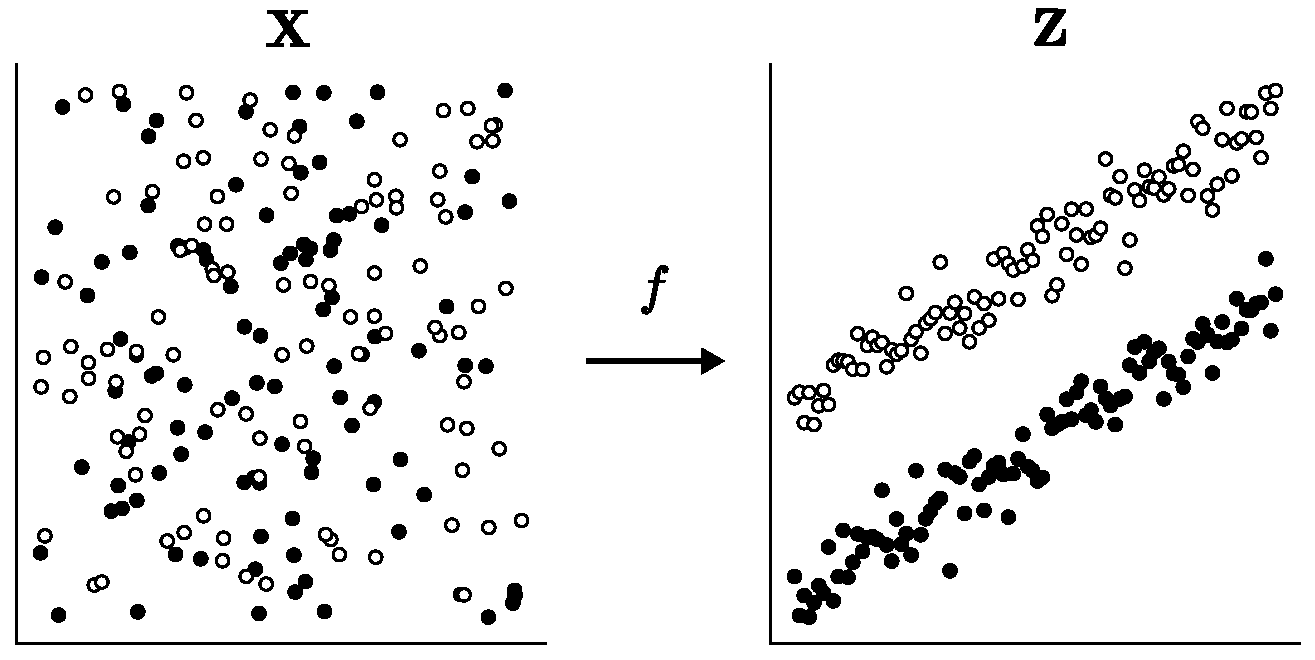
\includegraphics[width=9cm]{figures/representation_learning.pdf}
	 \caption{Illustration of representation learning (RL) as a function $f$, mapping vectors from a dimensional space to a representation space.}
	\label{}      
	\centering
\end{figure}

Mathematically, \ac{RL} is defined as a function $f : \mathbf{X} \to \mathbf{Z}$, that transforms the input data $\mathbf{X} = \{\mathbf{x}_1, \dots, \mathbf{x}_S\}$, into features $\mathbf{Z} = \{\mathbf{z}_1, \dots, \mathbf{z}_S\}$, where each vector $\mathbf{x}_s \in \mathbb{R}^n$ and its image $\mathbf{z}_s \in \mathbb{R}^p$, and $\mathbb{R}^p$ denotes the representation space.
The objective function $f$ leads the model to learn meaningful representations of the input data, preserving information, reducing redundancy and generally reducing dimensionality.

In recent years, many \ac{RL} methods have been proposed from different perspectives and families \cite{Balestriero2023}, 
e.g., contrastive learning methods (InfoNCE \cite{Tschannen2019,LeKhac2020,Aitchison2021}), deep metric learning (SimCLR \cite{Chen2020,Bachman2019}, NNCLR \cite{Dwibedi2021}, etc.), non-contrastive methods (VICReg \cite{Bardes2021}, BarlowTwins \cite{Zbontar2021,Lisaius2024}, etc), among others.
Such approaches are particularly useful in cases where the observed data is generated by a limited set of variables \cite{Coifman2006}. 
However, \ac{RL} is not limited to these families of methods, and conventional neural network models, such as autoenconders (AEs) can also form a representation learning method.

These approaches can also be seen as belonging to the field of self-supervised learning (SSL). Indeed, self-supervised learning techniques enable models to be pre-trained on unlabeled data, reducing reliance on labeled datasets. Furthermore, data augmentation techniques (rotations, translations, etc.) applied in these type of models have proven to improve performance without increasing the amount of training data.

\subsection{Autoencoders}\label{aes}
Autoencoders are a specific type of ANN used for unsupervised learning (Figure \ref{AEs_example}) \cite{Bank2020, Bank2023}. They have applications in various research fields, such as anomaly detection, data compression, and feature learning. Their aim is to encode the input into a compressed representation, and then reconstruct the input from this representation, so that the reconstruction is as similar as possible to the input \cite{Tzelepi2022,Zhang2019}. 
% Both under- and overcomplete versions exist, as well as variational AE \cite{Valero2021}. 

Although \ac{AEs} are not in principle designed for detection and classification tasks, several works have demonstrated their potential to ease these tasks by using \ac{AE}-derived data for change detection and binary classification models \cite{LopezFandino2018,Luppino2024,Kalinicheva2019}. Since \ac{AEs} are trained to compress and afterwards reconstruct the input data, they basically learn to model samples belonging to a certain joint distribution, leading the model to learn class-specific properties.

% Also, It has the capacity to adapt to changing environmental circumstances, which is critical in agriculture owing to the variability caused by factors like as seasonal shifts and weather conditions \cite{Ienco2017, Russwurm2018}. 

% The AEs are composed by the following elements:
% \begin{itemize}
% 	\item \textbf{Encoder}: The input data is passed through an encoder network, which reduces the dimensionality of the input and produces a compressed representation.
% 	\item \textbf{Code}: The output of the encoder is a compressed representation of the input data, also known as the "latent space" or "bottleneck." This encoding captures the essential features of the input in a low dimension space.
% 	\item \textbf{Decoder}: The code is passed through the decoder,  which aims to reconstruct the original input data. The decoder's architecture is typically a mirror image of the encoder, gradually expanding the dimensions back to match the original input.
% 	\item \textbf{Loss function}: The performance of an AE is typically measured by a loss function, which quantifies the difference between the input and the reconstructed output.
% 	\item \textbf{Training}: During training, the AE adjusts its weights to minimize the reconstruction error, effectively learning a compact representation of the input data.\\
% \end{itemize}

\begin{figure}[H]
	\centering
	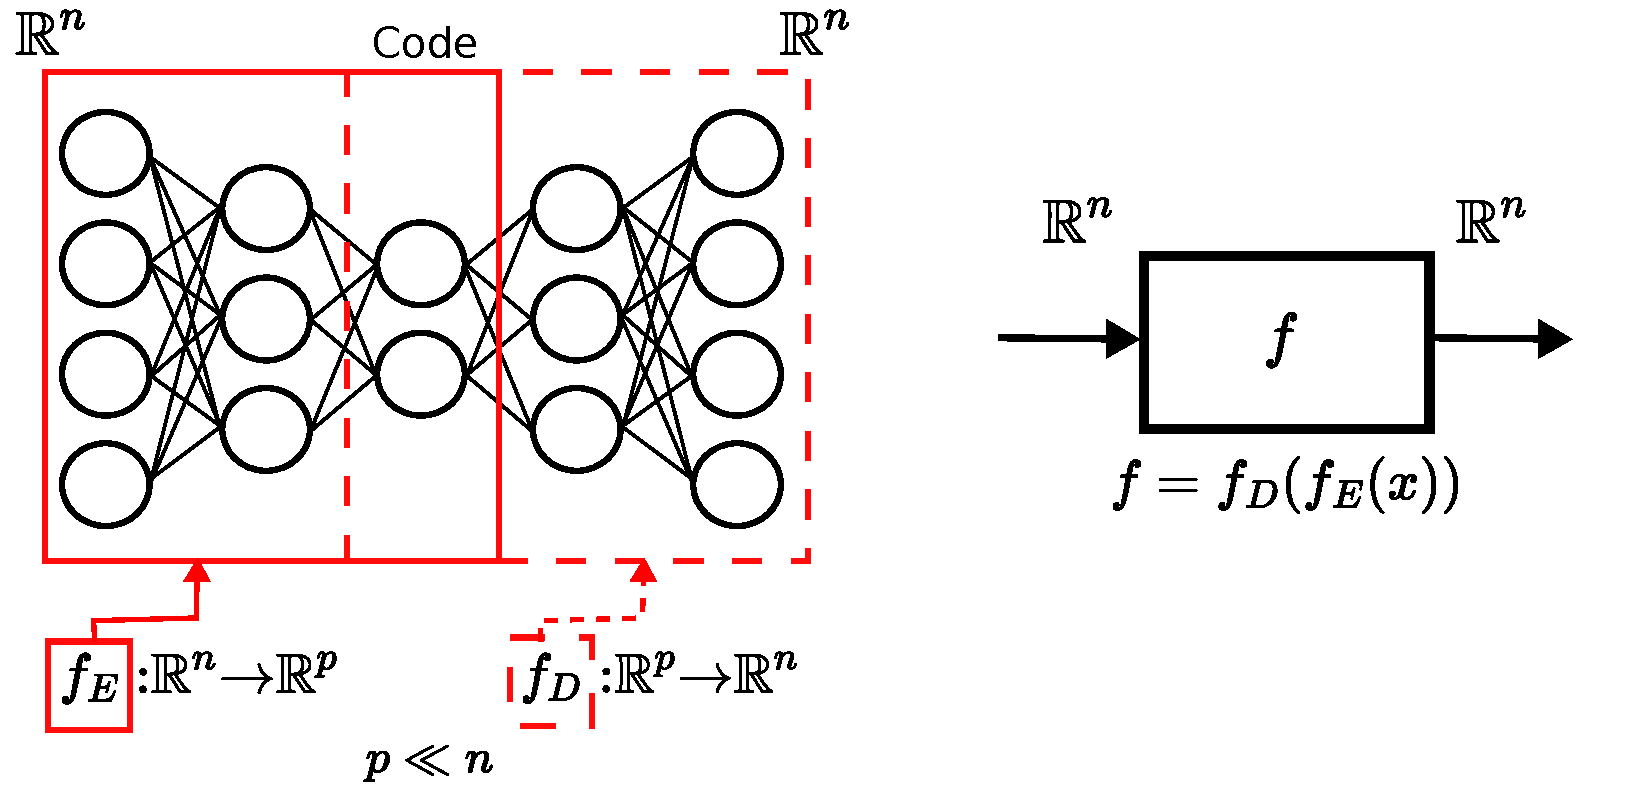
\includegraphics[width=8cm]{figures/autoencoder_methodology.pdf}
	 \caption{Example of an autoencoder architecture with mathematical definition as a function. In the present work, the reconstruction difference between input and output is used as representation, and not the code itself.}
	\label{AEs_example}      
	\centering
\end{figure}
% Self-supervised learning techniques, such as \ac{AEs}, enable models to be pre-trained on unlabeled data, reducing reliance on labeled datasets \cite{Ghanbarzadeh2024}. Furthermore, data augmentation techniques (rotations, translations, etc.) applied in these type of models have proven to improve performance without increasing the amount of training data \cite{Russwurm2018, Zhong2019, Zbontar2021}. 

The aim of the \ac{AEs}, formally defined in \cite{Baldi2012}, is to learn  the functions $f_{E}: \mathbb{R}^{n} \to \mathbb{R}^{p} $ and $f_{D}: \mathbb{R}^{p} \to \mathbb{R}^{n}$, where $f_{E}$ denotes the encoder function, $f_{D}$ is the decoder function, $n$ is the dimension of the input and output spaces, and $p$ denotes the dimension of the code space. Generally $p \ll n$, leading to learn compressed features of the data. 
% A characteristic of the AEs is that they are trained gradually layer by layer, therebefore, each hidden layer is seen as a regression model.

% \subsubsection{Encoder}
% The input data is passed through an encoder network, which reduces the dimensionality of the input and produces a compressed representation.
% This function $f_E$ maps the input data to the learned representation, each neuron is conected with all neurons of the next layer, 
% the conection between layers have a weight and bias  associeted and each neuron apply to the input one activation function alpha.
% Mathematically, it can be represented as:

% \begin{equation}
% 	f_{E_{i}}(x) = \alpha(w_{i}x + b_{i})
% \end{equation}
% where $i = 1,2, \dots , I$ is the number of layers, $w_{i}$ denotes the weight, $b_{i}$ is the bias and $\alpha$ denotes the activation function.
% Therefore, we can define $f_{E{i}} : \mathbb{R}^{n_{i-1}} \to \mathbb{R}^{n_{i}}$ considering $n_{i} < n_{i-1}$.

% % \begin{itemize}
% % 	\item Each neuron is conected with all neurons of the next layer.
% % 	\item The conection between layers have a weight $w_{i}$ and bias $b_{i}$ associeted.
% % 	\item Each neuron apply to the input one activation function $\alpha$
% % 	\item The adjust of the weights is with the backpropagation learing algorithm. 
% % \end{itemize} 

% \subsubsection{Bottleneck}
% The output of the encoder is a compressed representation of the input data, 
% also known as the "latent space" or "code." This encoding captures the essential 
% features of the input in a low dimension space. 

% % \begin{equation}
% % 	n_{1} = m_{J}                  
% % 	n_{2} = m_{j-1}                                 
% % 	\vdots                                       
% % 	n_{I} = m_{j} 
% % \end{equation}

% \subsubsection{Decoder}
% The code is passed through the decoder function $f_{D}$, which aims to reconstruct the original input data. 
% The decoder's architecture is typically a mirror image of the encoder, gradually expanding the 
% dimensions back to match the original input, therefore, they have a symmetric architecture. 
% This function is Mathematically defined as following:

% \begin{equation}
% 	f_{D_{j}}(x) = \alpha(w_{j}x + b_{j})
% \end{equation}
% where, $j = 1,2, \dots , J$ is the number of layers, $w_{j}$ denotes the weight, $b_{j}$ is the bias and $\alpha$ denotes the activation function.
% We define $f_{D{j}} : \mathbb{R}^{m_{j-1}} \to \mathbb{R}^{m_{j}}$ considering $m_{j} < m_{j-1}$.


% \subsubsection{Loss Function}
% The performance of an AE is typically measured by a loss function, which 
% quantifies the difference between the input and the reconstructed output.
% The loss function is typically defined using a distance metric, it can be mathematically defined as:

% % \begin{equation}
% % 	RE = L(X, \tilde{X}) %f_{D}(f_{E}(X)))
% % \end{equation}

% %where $L$ is a loss function, $X$ is the input data and $\tilde{X}$ is the reconstructed data.

% %Re = L(X,g(f(X)))

% \subsubsection{Training}
% During training, the AE adjusts its weights to minimize the reconstruction 
% error, effectively learning a compact representation of the input data.


% \begin{table}[H]
% 	\centering
% 	\small
% 	\begin{tabular}{c c c}
% 	   % &\begin{figure}\includegraphics[width=3cm]{Figures/concepts_images/AE_methodology_part2.pdf}\centering\end{figure}& \\
% 		\textbf{Encoder} & & \textbf{Decoder} \\ 
% 		Linear regression model & & Linear regression model\\ [1ex]
% 		$f_{i}(x) = \alpha(w_{i}x + b_{i})$ &  & $f_{j}(x) = \alpha(w_{j}x + b_{j})$ \\
% 		$i = 1,2, \dots , I$  & & $j = 1,2, \dots , J$ \\ 
% 		where $I$ is the number of layers & & where $J$ is the number of layers\\
% 		$f_{i} : \mathbb{R}^{n_{i-1}} \to \mathbb{R}^{n_{i}}$ & & $f_{j} : \mathbb{R}^{n_{j-1}} \to \mathbb{R}^{n_{j}}$\\ 
% 		$n_{i} < n_{i-1}$ &  $\Longleftarrow$  \textbf{Bottleneck} $\Longrightarrow$  & $m_{j} < m_{j_1}$\\
% 						  &   $n_{1} = m_{J}$                                & \\ 
% 						  & $n_{2} = m_{j-1}$                                & Symmetric architecture\\ 
% 						  & $\vdots$                                         & $I = J$\\  
% 						  & $n_{I} = m_{j}$                                  & \\ 
% 	\end{tabular}
% 	\caption{}
% \end{table}

\section{Proposed method}
Consider an annual multi-spectral time series dataset acquired by an optical sensor, i.e., each sample has been acquired at different times. From the entire set of observations, only a subset will usually be useful as weather conditions such as clouds, cirrus, cloud shadows, snow, among others, occasionally obstruct the land surface. 
Missing data produced by these conditions commonly leads to poor performance on particular tasks, such as land use / land cover classification or change detection.
Therefore, it is of utmost importance to extract and  use only the land related information, either by filtering the data, or generating new features (often in the form of composites).

\subsection{Problem statement}
Let $\mathscr{X} \in \mathbb{R}^{P \times B \times T}$ be a multispectral time series dataset represented as a third-order array, where $P$ represents the number of geographic points on the earth surface, $B$ is the number of spectral bands, and $T$ denotes the number of temporal observations, and each geographic point is denoted as a vector $\mathbf{x} \in \mathbb{R}^{B \cdot T}$ and $\mathbf{x} \in \mathscr{X}$. The aim is to transform each vector $\mathbf{x}$ into a representation vector $\mathbf{z} \in \mathbb{R}^{R}$, where $R$ is the number of new features named representations. The representation vector $\mathbf{z}$ addresses label scarcity and missing data produced by clouds, and permits downstream tasks such as crop type classification (See Figure \ref{bigpicture}).

\begin{figure}[H]
	\centering
	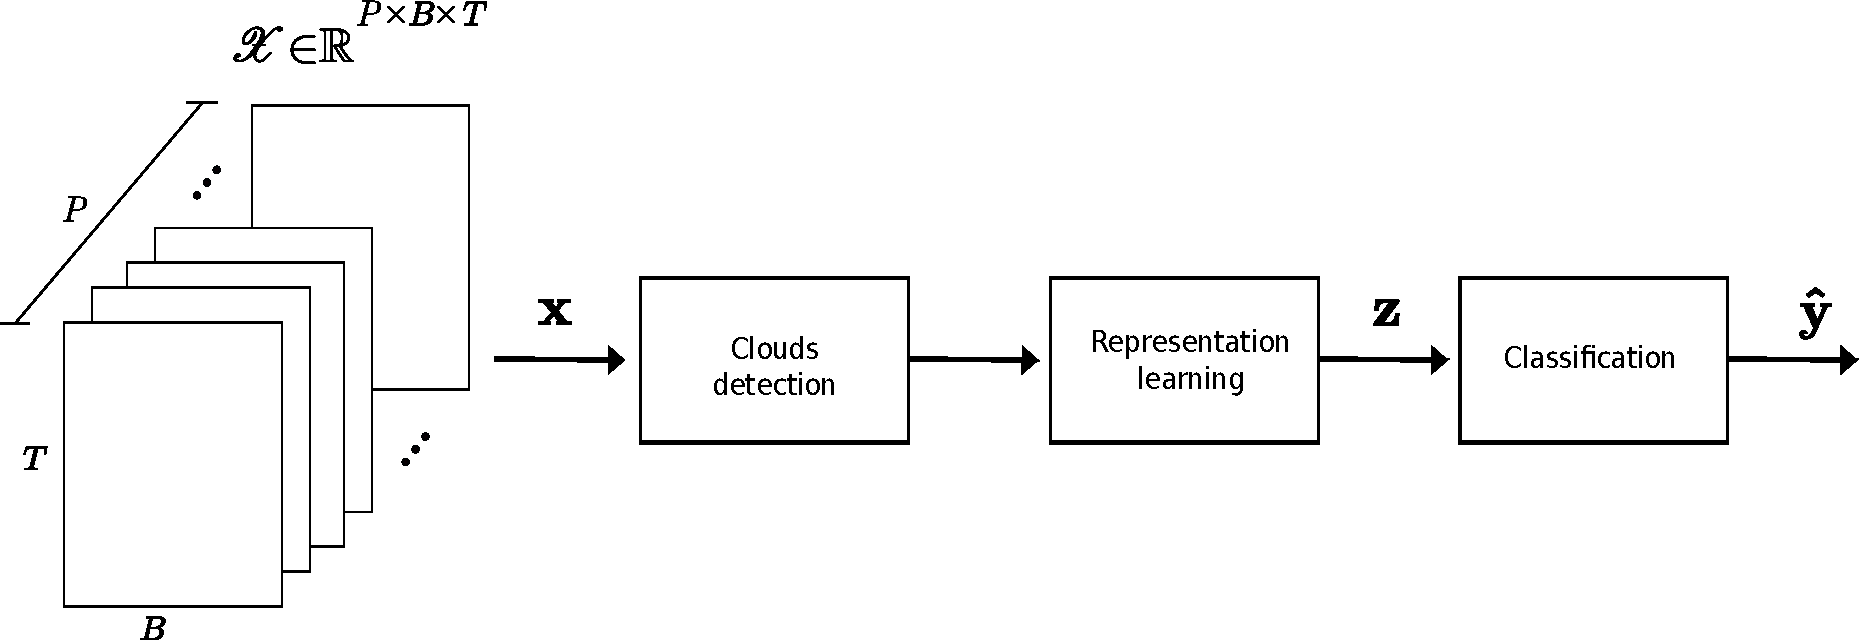
\includegraphics[width=10cm]{figures/bigpicture_with_clement.pdf}
	\caption{First level of the proposed workflow. Scene classification product provided by the European Space Agency (ESA) is used to mask out cloudy samples from a geographic point (pixel) shaped as a $T \times B$ array. 
    %DIF <  The pixel cloud free observations are the inputs to generate a representations vector, which is a concatenation of the reconstruction differences per autoencoder, and are then the input data to a classification model.
    %DIF >  The pixel cloud-free observations are the inputs to generate a representations vector, which is a concatenation of the reconstruction differences per autoencoder, and are then the input data to a classification model.
\DIFaddbeginFL \DIFaddFL{Figure 3.    }\DIFaddendFL }
	\label{bigpicture}
	\centering
\end{figure}

\subsection{Methodology}
The methodology of this work consists of four processes: data downloading and preprocessing, model training, inference (representations formation) and, as downstream task to evaluate the quality of the derived representations, classification. The proposed framework is shown in more detail in Figure \ref{abstract}.
\begin{figure}[H]
	\centering
	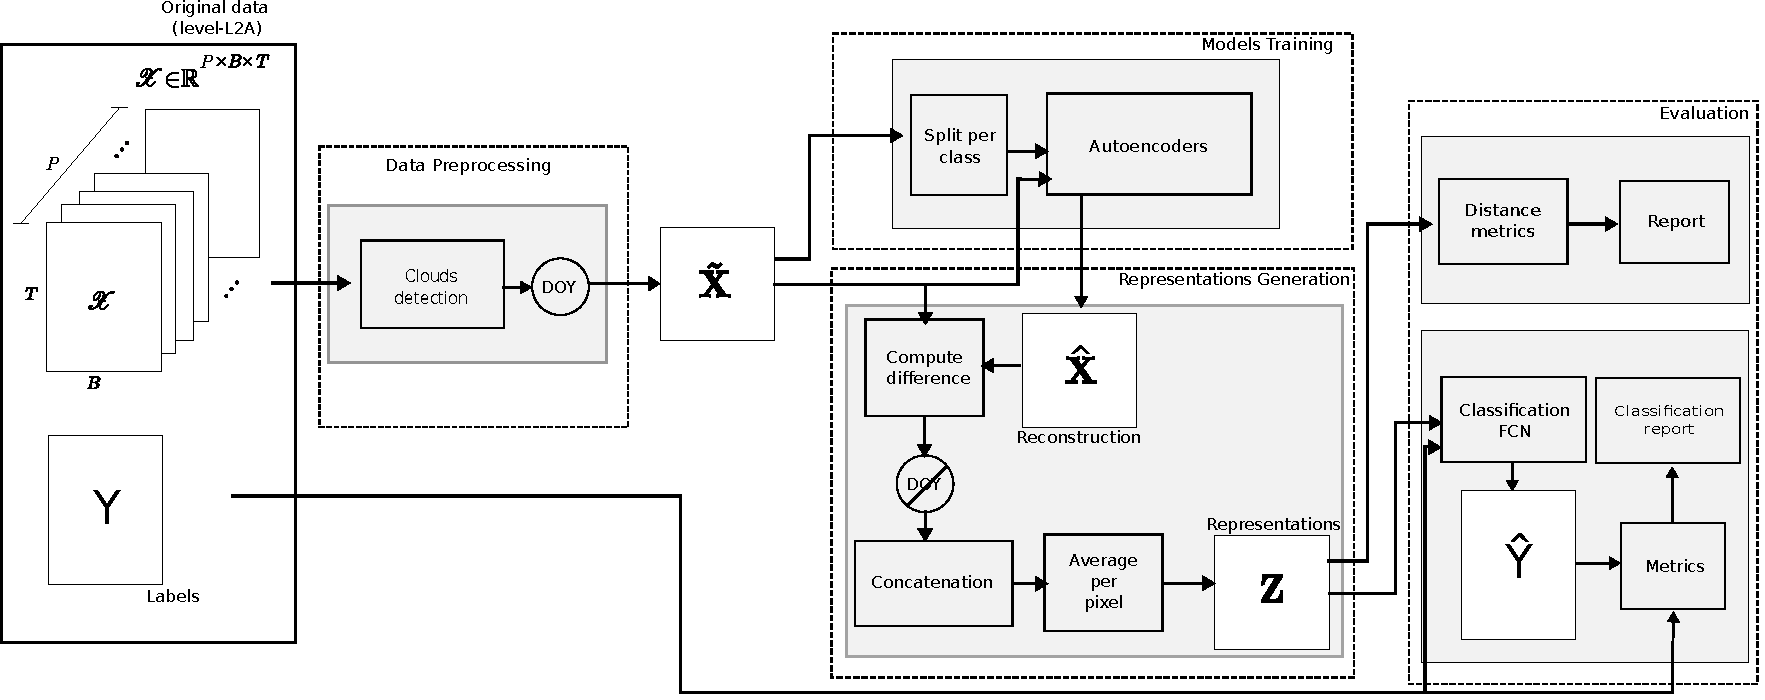
\includegraphics[width=\textwidth]{figures/abstract.pdf}
	\caption{Proposed framework block diagram. The full methodology is composed by four main blocks: data preprocessing, model training, representation generation and evaluation.} 
	\label{abstract}
\end{figure}
\subsubsection{Data downloading/preprocessing}\label{data_preprocessing}
Reference crop type labels were extracted from a public benchmark dataset named BreizhCrops \cite{Russwurm2020} (field level).
Google earth engine (GEE) was used to download full multitemporal multispectral data from a region of interest (ROI) (see Figure \ref{GEE_process}). \\
\begin{figure}[H]
	\centering
	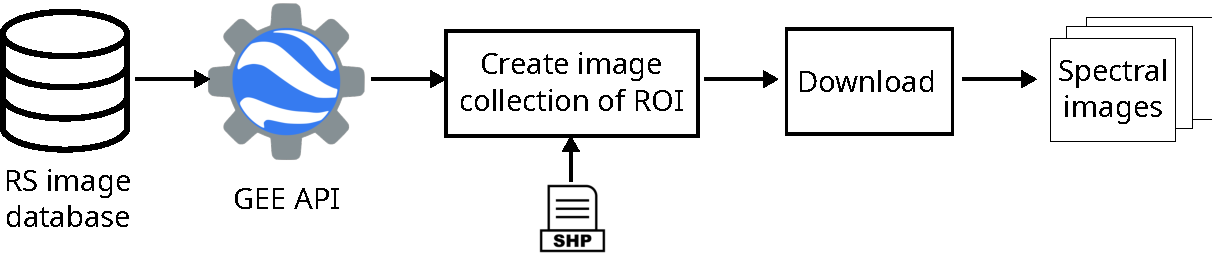
\includegraphics[width=0.6\textwidth]{figures/gee_download.pdf}
	\caption{Dataset downloading process using the google earth engine (GEE) database.}
	\label{GEE_process}    
\end{figure}

Given the multispectral time series, a scene classification product (e.g., \DIFaddbegin \DIFadd{ESAs }\DIFaddend sen2cor) is used to get a cloud/non-cloud mask for each sample $\mathbf{x}$, i.e., for each temporal observation at pixel level.
Cloudy samples are excluded from the dataset. This creates a set of pixels with variable number of \DIFdelbegin \DIFdel{cloud free }\DIFdelend \DIFaddbegin \DIFadd{cloud-free }\DIFaddend (temporal) observations. Only the \DIFdelbegin \DIFdel{cloud free }\DIFdelend \DIFaddbegin \DIFadd{cloud-free }\DIFaddend observations of a pixel are the inputs to generate a representations vector. This makes our model flexible and independent on the number of clear observations.

To leverage the temporal information for the particular task of crop type classification, we add temporal embeddings to each sample, with the aim to extend the vector space to one where similar spectral curves of different crop types at different growth stages are separable. 
We use the sine and cosine functions to model the annual periodic phenomenon presented by the cyclical character of the nature seasons and crops evolution between planting and harvest. As day 1 and 365 are in principle distant but with similar natural conditions, we \DIFdelbegin \DIFdel{scaled }\DIFdelend \DIFaddbegin \DIFadd{embed time by scaling }\DIFaddend the acquisition day-of-year (\ac{DOY}) to (0, 1) range dividing by 365 and then place them on a real value scale by computing the sine and cosine. This makes each scaled \ac{DOY} a unit vector decomposed into two orthogonal vectors, regarded as spring–fall axis (sine), and summer–winter axis (cosine) giving to our method the capacity to perform correctly in different earth latitudes \cite{Dahlin2016}.

Hence, each sample $\mathbf{\tilde{x}} \in \mathbb{R}^F$
has $F$ features, i.e., $B$ spectral bands plus two values denoting the sensing \ac{DOY}, computed as follows
\begin{equation}
	doy_{\sin} = \left(\sin\left(\frac{2\pi doy}{365}\right)+1\right)/2
\end{equation}
and
\begin{equation}
	doy_{\cos} = \left(\cos\left(\frac{2\pi doy}{365}\right)+1\right)/2, 
\end{equation}
where $doy$ denotes the \ac{DOY} as a numeric value from 1 to 365, and $doy_{\sin}$ and $doy_{\cos}$ are in the range 0 to 1.
	% \item Inference: In this part of the proposed framework,the representations are generated using the AEs trained. Given as a input individual temporal observation free of clouds to the AEs, after that, generating the recostruction and computing the error beteween input and recostruction, deleting the day of the year (DOY) and computing the average per pixel to generate the representations $\mathbf{Z}$.
	% \item Evaluation: There are two option, the first is to use distance metrics for evaluate the separability between classes and the second is to do a classification using a FCN and after that evaluate the prediction usign metrics for performance evaluation.

\subsubsection{Model training}\DIFaddbegin \label{training}
\DIFaddend The principle of this work is to train a set of $C$ independent AEs with vectors $\mathbf{\tilde{x}}_c$, which are individual time-tagged spectral signatures of cloud/shadows-free observations that belong to a particular class \DIFdelbegin \DIFdel{/cluster }\DIFdelend $c$ for $c=1,\dots,C$,  resulting in $C$ semi-supervised trained models able to reconstruct samples from the same class\DIFdelbegin \DIFdel{/cluster}\DIFdelend , approaching the reconstruction difference \DIFdelbegin \DIFdel{vector to zero}\DIFdelend \DIFaddbegin \DIFadd{to the zero vector}\DIFaddend , while using the ensemble of reconstruction difference vectors to derive the representations (see Figure \ref{errors}).

\begin{figure}[H]
	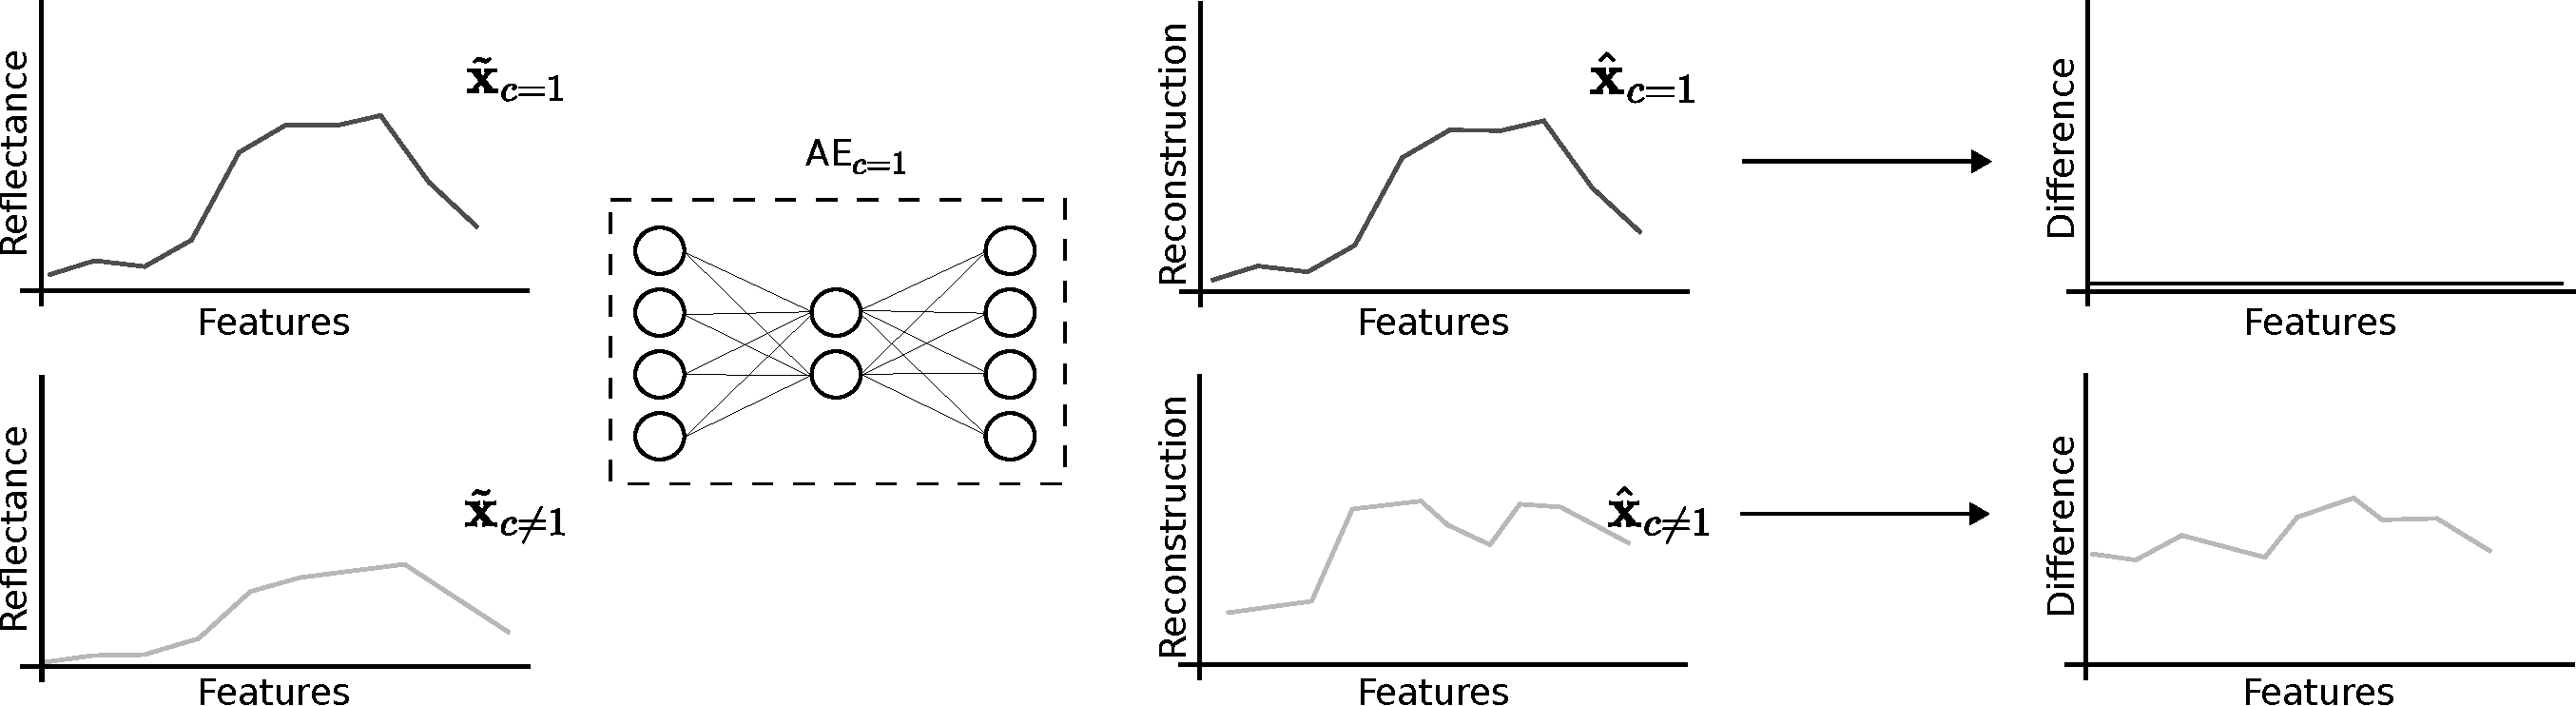
\includegraphics[width=\textwidth]{figures/AE_example_corrected.pdf}
	\caption{Example of the expected output for positive and negative samples. The \DIFdelbeginFL \DIFdelFL{"}\DIFdelendFL difference \DIFdelbeginFL \DIFdelFL{" }\DIFdelendFL from the ensemble of autoencoders (AEs) constitute the representations for the downstream task.}
	\label{errors}
\end{figure}
The training process of the AEs can be semi-supervised, given a labeled dataset, as in this work, or unsupervised, with no ground truth data (e.g., by training a set of random \ac{AEs} not associated to specific crop types or classes). 
The scope of this work addresses the semi-supervised approach, with a crop type labeled dataset as pairs $(x,y)$, where $y$ is an integer value which indicates the class that $x$ belongs to. Samples are split in as many subdatasets as classes and each subdataset is used to train a different AE.
This process is graphically represented in Figure \ref{abstract} as model training and further illustrated in Figure \ref{aes_train}.

\begin{figure}[H]
	\centering
	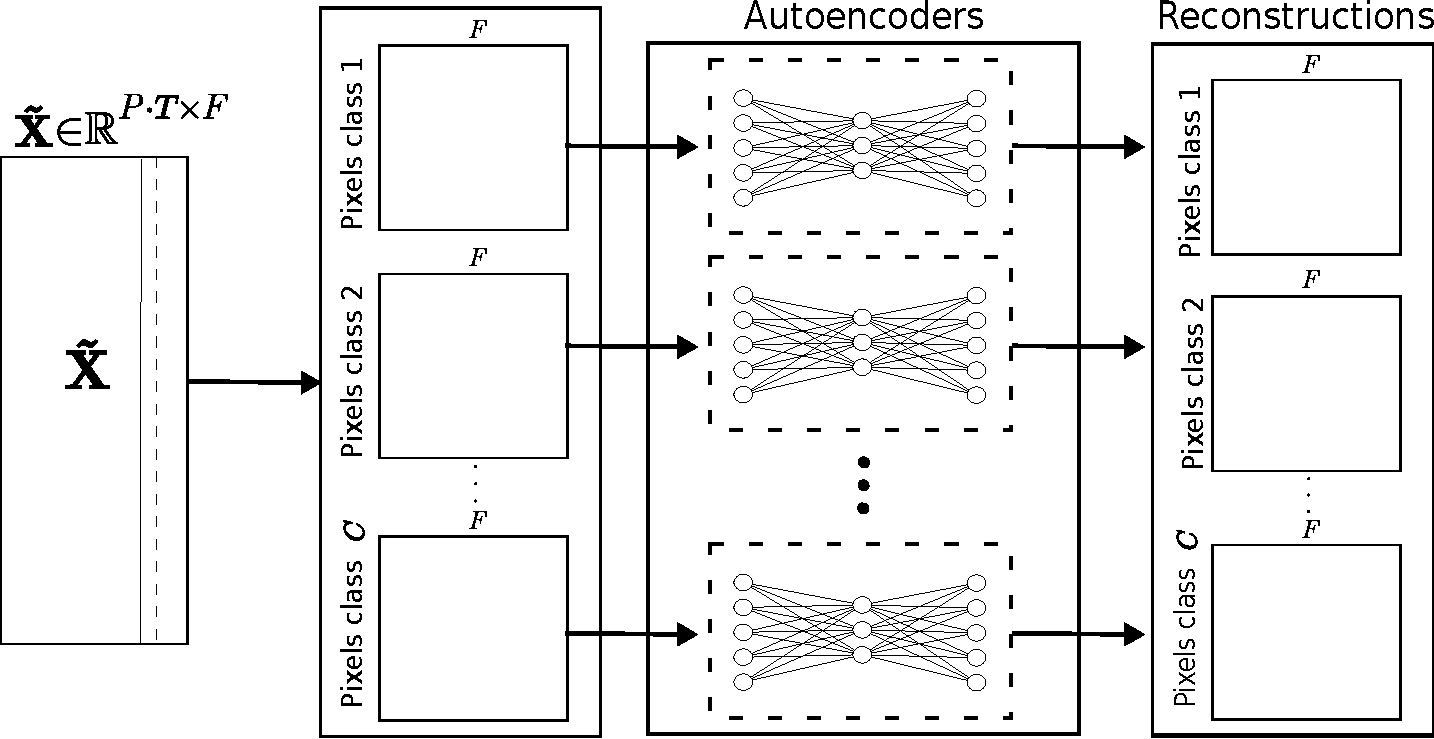
\includegraphics[width=0.7\textwidth]{figures/training.pdf}
	\caption{Autoencoders (AEs) training. Each autoencoder is trained with a \DIFaddbeginFL \DIFaddFL{finite }\DIFaddendFL set of individual spectral curves belonging to one of the crop types. The reconstructions from the $C$ classes are used to calculate the difference vector across the ensemble, that is the final set of representations.}    
	\label{aes_train}      
\end{figure}

As mentioned in Section \ref{aes}, an AE is formally defined as a \DIFdelbegin \DIFdel{composed function $f(x) = f_D(f_E(x))$}\DIFdelend \DIFaddbegin \DIFadd{composite function $f_{AE}(\mathbf{x}) = f_D(f_E(\mathbf{x}))$}\DIFaddend . For our input vectors \DIFdelbegin \DIFdel{$\mathbf{\tilde{x}}_c$}\DIFdelend \DIFaddbegin \DIFadd{$\mathbf{\tilde{x}}$}\DIFaddend , each AE can be seen as a function
\begin{equation}
	f\DIFaddbegin \DIFadd{_{AE}}\DIFaddend (\mathbf{\tilde{x}}\DIFdelbegin \DIFdel{_c}\DIFdelend ) = f_D(f_E(\mathbf{\tilde{x}}\DIFdelbegin \DIFdel{_c}\DIFdelend ))) \DIFaddbegin \DIFadd{= \mathbf{\hat{x}}
}\DIFaddend \end{equation}
where, \DIFdelbegin \DIFdel{$f_E(\mathbf{\tilde{x}}_c)$ }\DIFdelend \DIFaddbegin \DIFadd{$f_E(\mathbf{\tilde{x}})$ }\DIFaddend denotes the encoder function, which maps the input vectors\DIFdelbegin \DIFdel{that belong to class $c$}\DIFdelend , from the input space $\mathbb{R}^F$ to an embedding space $\mathbb{R}^P$, known as code, and \DIFdelbegin \DIFdel{, at the same time, is a composed function of the hidden layers $f_{E_i}$
}\begin{displaymath}
	\DIFdel{f_E(\mathbf{\tilde{x}}_c) = f_{E_{I}}(f_{E_{I-1}}(\dots (f_{E_{1}}(\mathbf{\tilde{x}}_c))))
	%DIFDELCMD < \label{composed}%%%
}\end{displaymath}%DIFAUXCMD
\DIFdel{where $f_{E_{i}}(\cdot)$, for $i = 1, \dots, I$ are regression functions }\begin{displaymath}
	\DIFdel{f_{E_{i}}(\mathbf{y}_{i-1}) = \alpha_i(\mathbf{W}_{i}\mathbf{y}_{i-1} + \mathbf{b}_{i})
}\end{displaymath}%DIFAUXCMD
\DIFdel{where $i$ denotes the layer number, $\mathbf{y}_{i-1}$ stands for the output of layer $i-1$, $\mathbf{W}_{i}$ and $\mathbf{b}_{i}$ denotes the weights and bias at layer $i$ respectively, and $\alpha_i$ the activation function.
}%DIFDELCMD < 

%DIFDELCMD < %%%
\DIFdel{The decoder function }\DIFdelend $f_D(\cdot)$ \DIFdelbegin \DIFdel{, also a composed function as $f_E(\cdot)$ in eq. \ref{composed},
maps the code to an estimated reconstruction of the input vector by
}\DIFdelend \DIFaddbegin \DIFadd{maps the code to an estimated reconstruction $\mathbf{\hat{x}}$ of the input vector.
Since our architecture has $C$ }\ac{AE}\DIFadd{s, then it has $C$ composite functions $f_{AE}^{(c)}$, for $c=1,2,\dots,C$. Each }\ac{AE} \DIFadd{is trained with a set of vectors belonging to a single class, and consequently a particular $f_{AE}^{(c)}$ is learned. In general,
}\DIFaddend \begin{equation}
    \mathbf{\hat{x}}\DIFaddbegin \DIFadd{_c^{(c)} }\DIFaddend = f\DIFdelbegin \DIFdel{_{D}(f_E}\DIFdelend \DIFaddbegin \DIFadd{_{AE}^{(c)}}\DIFaddend (\DIFdelbegin \DIFdel{\mathbf{\mathbf{\tilde{x}}}}\DIFdelend \DIFaddbegin \DIFadd{\mathbf{\tilde{x}}}\DIFaddend _c)
\DIFdelbegin \DIFdel{)
}\DIFdelend \end{equation}
where \DIFdelbegin \DIFdel{$\mathbf{\hat{x}}$ is the approximation of }\DIFdelend \DIFaddbegin \DIFadd{$\mathbf{\tilde{x}}_c$ denotes }\DIFaddend the input vector \DIFdelbegin \DIFdel{, updating the weights $\mathbf{W}_i$ and bias $\mathbf{b}_i$ by backpropagating the loss $d$ computed by a loss function $L$ as
}\begin{displaymath}
	\DIFdel{d = L(\mathbf{\tilde{x}}_c, f_D(f_E(\mathbf{\tilde{x}}_c))) = L(\mathbf{\tilde{x}}_c, \mathbf{\hat{x}})
	%DIFDELCMD < \label{loss}%%%
}\end{displaymath}%DIFAUXCMD
\DIFdel{where $L$ computes the distance between $\mathbf{\tilde{x}}_c$ and $\mathbf{\hat{x}}$, and $\mathbf{W}_i$ and $\mathbf{b}_i$ are updated approaching $d \to 0$, by an optimization algorithm such as stochastic gradient descent, Adam or Adagrad. 
}\DIFdelend \DIFaddbegin \DIFadd{belonging to class $c$, $f_{AE}^{(c)}$ is the }\ac{AE} \DIFadd{function associated to the $c$-th class, and $\mathbf{\hat{x}}_c^{(c)}$ is the output vector delivered by the $c$-th }\ac{AE}\DIFadd{. 
%DIF >  Each \ac{AE} is trained using a loss function
%DIF >  , and, at the same time, is a composite function of the hidden layers $f_{E_i}$
%DIF >  \begin{equation}
%DIF >  	f_E(\mathbf{\tilde{x}}_c) = f_{E_{I}}(f_{E_{I-1}}(\dots (f_{E_{1}}(\mathbf{\tilde{x}}_c))))
%DIF >  	\label{composed}
%DIF >  \end{equation}
%DIF >  where $f_{E_{i}}(\cdot)$, for $i = 1, \dots, I$ are regression functions
%DIF >  \begin{equation}
%DIF >  	f_{E_{i}}(\mathbf{y}_{i-1}) = \alpha_i(\mathbf{W}_{i}\mathbf{y}_{i-1} + \mathbf{b}_{i})
%DIF >  \end{equation}
%DIF >  where $i$ denotes the layer number, $\mathbf{y}_{i-1}$ stands for the output of layer $i-1$, $\mathbf{W}_{i}$ and $\mathbf{b}_{i}$ denotes the weights and bias at layer $i$ respectively, and $\alpha_i$ the activation function.
}

%DIF >  The decoder function $f_D(\cdot)$, also a composite function as $f_E(\cdot)$ in eq. \ref{composed}, maps the code to an estimated reconstruction of the input vector by
%DIF >  \begin{equation}
%DIF >  	\mathbf{\hat{x}} = f_{D}(f_E(\mathbf{\mathbf{\tilde{x}}}_c))
%DIF >  \end{equation}
%DIF >  where $\mathbf{\hat{x}}$ is the approximation of the input vector, updating the weights $\mathbf{W}_i$ and bias $\mathbf{b}_i$ by backpropagating the loss $d$ computed by a loss function $L$ as

%DIF >  \begin{equation}
%DIF >  	d = L(\mathbf{\tilde{x}}_c, f_D(f_E(\mathbf{\tilde{x}}_c))) = L(\mathbf{\tilde{x}}_c, \mathbf{\hat{x}})
%DIF >  	\label{loss}
%DIF >  \end{equation}
%DIF >  where $L$ computes the distance between $\mathbf{\tilde{x}}_c$ and $\mathbf{\hat{x}}$, and $\mathbf{W}_i$ and $\mathbf{b}_i$ are updated approaching $d \to 0$, by an optimization algorithm such as stochastic gradient descent, Adam or Adagrad.
\DIFaddend 

\subsubsection{Representations generation (Inference)}\DIFaddbegin \label{methodology:inference}
\DIFaddend Given the $C$ trained \DIFdelbegin %DIFDELCMD < \ac{AEs}%%%
\DIFdelend \DIFaddbegin \ac{AE}\DIFadd{s}\DIFaddend , denoted as \DIFdelbegin \DIFdel{$f_c$}\DIFdelend \DIFaddbegin \DIFadd{$f_{AE}^{(c)}$}\DIFaddend , the set of \DIFdelbegin \DIFdel{cloud free }\DIFdelend \DIFaddbegin \DIFadd{cloud-free }\DIFaddend observations of individual geographic points (pixels) \DIFdelbegin \DIFdel{form }\DIFdelend \DIFaddbegin \DIFadd{forms }\DIFaddend an array $\mathbf{\tilde{X}} \in \mathbb{R}^{t \times F}$, where $t$ denotes the number of \DIFdelbegin \DIFdel{cloud free }\DIFdelend \DIFaddbegin \DIFadd{cloud-free }\DIFaddend samples for a given pixel. $\mathbf{\tilde{X}}$ is the input to \DIFdelbegin \DIFdel{all the }%DIFDELCMD < \ac{AEs}%%%
\DIFdelend \DIFaddbegin \DIFadd{the }\ac{AE}\DIFadd{s functions}\DIFaddend , and the reconstruction array is obtained from each AE as
\begin{equation}
	\mathbf{\hat{X}}\DIFdelbegin \DIFdel{_c }\DIFdelend \DIFaddbegin \DIFadd{^{(c)} }\DIFaddend = f\DIFdelbegin \DIFdel{_c}\DIFdelend \DIFaddbegin \DIFadd{_{AE}^{(c)}}\DIFaddend (\mathbf{\tilde{X}})
\end{equation}
where \DIFdelbegin \DIFdel{$\mathbf{\hat{X}}_c$ }\DIFdelend \DIFaddbegin \DIFadd{$\mathbf{\hat{X}}^{(c)}$ }\DIFaddend represents the reconstruction estimated by \DIFdelbegin \DIFdel{AE }\DIFdelend \DIFaddbegin \DIFadd{the }\DIFaddend $c$\DIFdelbegin \DIFdel{. }\DIFdelend \DIFaddbegin \DIFadd{-th }\ac{AE}\DIFadd{. 
}

\DIFaddend Then, the \DIFdelbegin \DIFdel{difference vector is computed by
the same loss function used in training phase (eq. \ref{loss}) as
}\DIFdelend \DIFaddbegin \DIFadd{$t$ difference vectors associated to a single pixel which form an array $\mathbf{D}^{(c)}$ are computed by
}\DIFaddend \begin{equation}
    \mathbf{D}\DIFdelbegin \DIFdel{_c }\DIFdelend \DIFaddbegin \DIFadd{^{(c)} }\DIFaddend = \DIFdelbegin \DIFdel{L(\mathbf{\tilde{X}}, \mathbf{\hat{X}}_c)
}\DIFdelend \DIFaddbegin \abs{\mathbf{\tilde{X}} - \mathbf{\hat{X}}^{(c)}}\DIFadd{^{\text{abs}}
}\DIFaddend \end{equation}
\DIFdelbegin \DIFdel{and }\DIFdelend \DIFaddbegin \DIFadd{where $d_{ij}^{(c)} = \text{abs}(\tilde{x}_{ij} - \hat{x}^{(c)}_{ij})$. Let $\mathbf{d}_i^{(c)}$ be the rows of $\mathbf{D}^{(c)}$, then }\DIFaddend the pixel mean reconstruction difference vector \DIFdelbegin \DIFdel{$\mathbf{\bar{d}}_c$ }\DIFdelend \DIFaddbegin \DIFadd{$\mathbf{\bar{d}}^{(c)} \in \mathbb{R}^F$ }\DIFaddend is computed by
\begin{equation}
	\mathbf{\bar{d}}\DIFdelbegin \DIFdel{_c }\DIFdelend \DIFaddbegin \DIFadd{^{(c)} }\DIFaddend = \frac{1}{t}\sum\DIFdelbegin \DIFdel{_{s=0}}\DIFdelend \DIFaddbegin \DIFadd{_{i=1}}\DIFaddend ^{t}\mathbf{d}\DIFdelbegin \DIFdel{_{sc}
}\DIFdelend \DIFaddbegin \DIFadd{_{i}^{(c)}
}\DIFaddend \end{equation}
\DIFdelbegin \DIFdel{where $\mathbf{d}_{sc}$ denotes the $s$-th row of $\mathbf{D}_c$ }\DIFdelend and the \DIFdelbegin \DIFdel{representations are formed by concatenating the mean pixel reconstruction difference vector as
}\DIFdelend \DIFaddbegin \DIFadd{representation $\mathbf{z}$ of the pixel $\mathbf{\tilde{X}}$ is formed by the concatenation of the $C$ vectors $\mathbf{\bar{d}}^{(c)}$ as
}\DIFaddend \begin{equation}
    \mathbf{z}=\mathbf{\bar{d}}\DIFdelbegin \DIFdel{_1 }\DIFdelend \DIFaddbegin \DIFadd{^{(1)} }\DIFaddend \oplus \mathbf{\bar{d}}\DIFdelbegin \DIFdel{_2 }\DIFdelend \DIFaddbegin \DIFadd{^{(2)} }\DIFaddend \oplus \cdots \oplus \mathbf{\bar{d}}\DIFdelbegin \DIFdel{_C
}\DIFdelend \DIFaddbegin \DIFadd{^{(C)}
}\DIFaddend \end{equation}
where $\oplus$ denotes the vector concatenation and \DIFdelbegin \DIFdel{$\mathbf{\bar{d}_c}$ the mean pixel reconstruction difference vector from AE $c$}\DIFdelend \DIFaddbegin \DIFadd{$\mathbf{z} \in \mathbb{R}^{R}$}\DIFaddend .
The inference phase of our proposed framework is presented in Figure \ref{Inference}\DIFaddbegin \DIFadd{.
}\DIFaddend \begin{figure}[H]
	\centering
	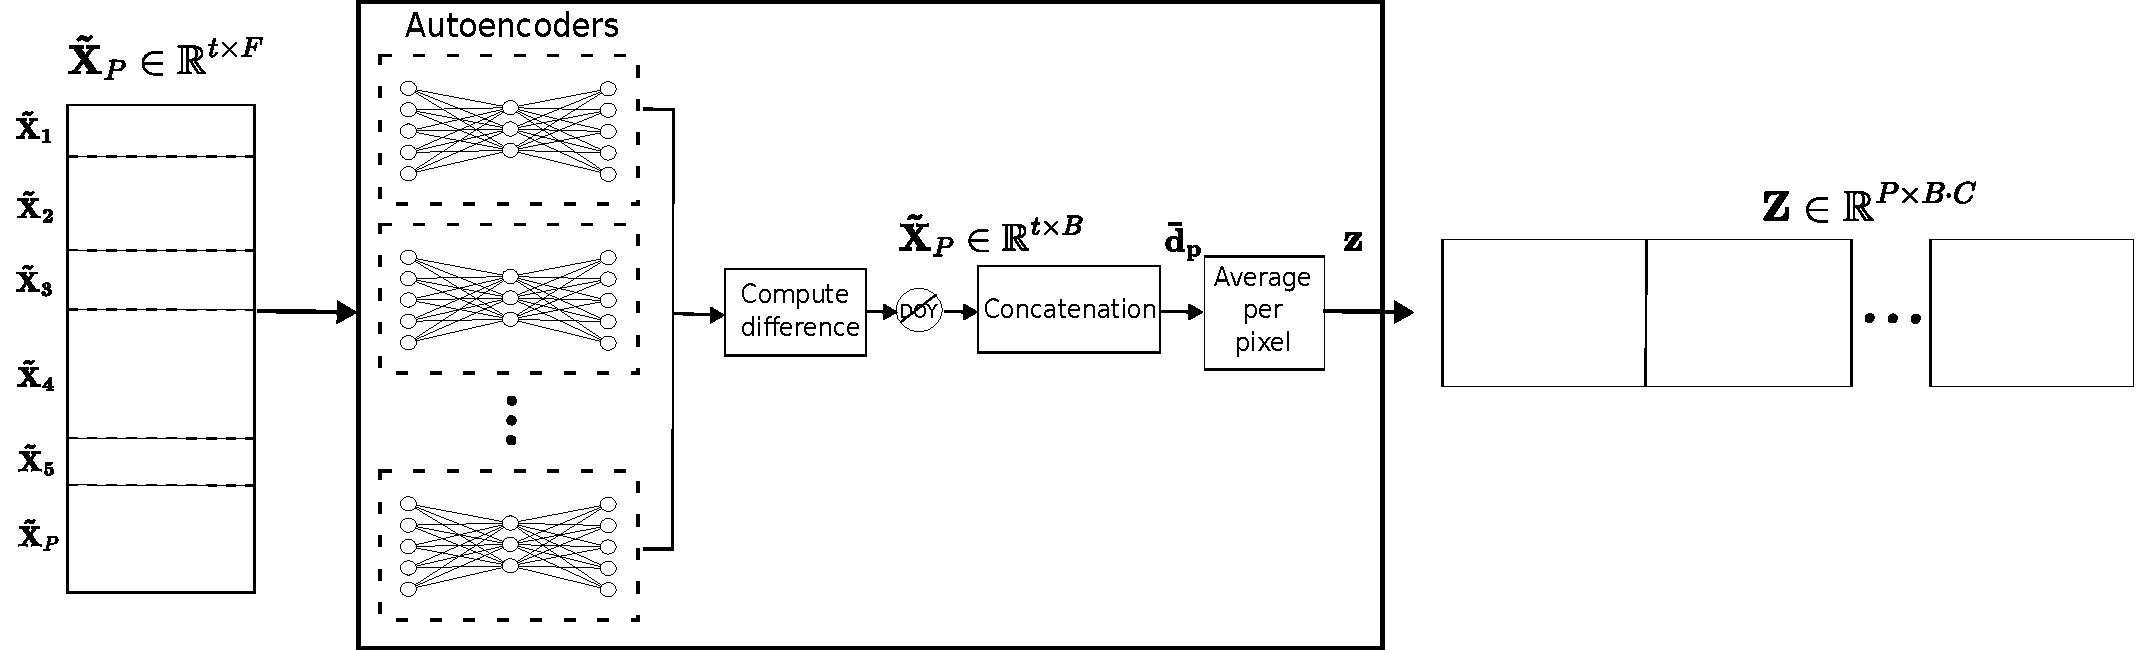
\includegraphics[width=\textwidth]{figures/testing.pdf}
	\caption{Inference workflow of the proposed framework. For each temporal set of cloud-free reflectance spectra, the average reconstruction difference vector are calculated for each of the $C$ autoencoders (AEs) and concatenated to define the representations of this pixel.}
	\label{Inference}    
\end{figure}

%%%%%%%%%%%%%%%%%%%%%%%%%%%%%%%%%%%%%%%%%%
\section{Experimental results}
\subsection{Dataset}\label{dataset}
\DIFdelbegin \DIFdel{For this work the }\DIFdelend \DIFaddbegin \DIFadd{The }\DIFaddend public benchmark dataset \textit{Breizhcrops} presented in \cite{Russwurm2020} was used for experiments and evaluation. This dataset is available at the GitHub repository
(\url{https://github.com/dl4sits/breizhcrops}). The provided multi-temporal multi-spectra data is from the Brittany region in the northwest of France and is composed of labeled Sentinel-2 images from January 1st to December 31st, 2017. Labels are assigned to the "average of reflectance values over the bounds of the field geometry retrieved from the dataset" \cite{Russwurm2020}.

This dataset is organized in four regions (see Table \ref{Regions}),
% by the "Nomenclature des Unités Territoriales Statistiques" (NUTS) system (see Table \ref{Regions}): Côtes-d’Armor (FRH01), Finistère (FRH02), Ille-et-Vilaine (FRH03),and Morbihan (FRH04)
and each region contains nine crop categories: barley, wheat, rapeseed, corn, sunflower, orchards, nuts, permanent meadows and temporary meadows.
\DIFdelbegin \DIFdel{To allow a direct comparison to the work published in \mbox{%DIFAUXCMD
\cite{Russwurm2020}}\hskip0pt%DIFAUXCMD
, we use the }\DIFdelend \DIFaddbegin \DIFadd{In \mbox{%DIFAUXCMD
\cite{Russwurm2020}}\hskip0pt%DIFAUXCMD
, }\DIFaddend regions FRH01 and FRH02 \DIFaddbegin \DIFadd{were used }\DIFaddend for training, FRH03 for validation, and FRH04 for evaluation.
% The data split is described in Table \ref{data_split}, which outlines the features employed in this experiment. These include DOY (sin and cosine), 10 spectral bands (10 and 20 meters resampled to 10m) and five well-known spectral indices (NDWI, NDVI, NDTI, NDSVI and EVI).

% \begin{table}[H]
% 	\caption{Regions of Britany with number of field parcels and time series for the atmospherically corrected surface reflectances at the bottom-of-atmosphere (L2A) \cite{Russwurm2020}.}
% 	\centering
% 	\begin{tabular}{c  c  c  c} 
% 		\hline
% 		Regions     & NUTS-3 & Parcels   & L2A \\ [1ex] 
% 		\hline
% 		Côtes-d'Armor   & FRH01  & $221,095$ & $178,632$ \\ [1ex]
% 		Finistère       & FRH02  & $180,565$ & $140,782$ \\ [1ex]
% 		Ille-et-Vilaine & FRH03  & $207,993$ & $166,367$ \\ [1ex]
% 		Morbihan		& FRH04  & $158,522$ & $122,708$ \\ [1ex] 
% 		\hline
% 		Total			&		 & $768,175$ & $608,489$ \\ [1ex] 
% 		\hline
% 	\end{tabular}
% 	\label{Regions}
% \end{table}
\begin{table}[H]
	\caption{Regions of Brittany (France) with number of field parcels and spectral data for the atmospherically corrected surface reflectances at the bottom-of-atmosphere (L2A) \cite{Russwurm2020}. The regions FRH01 and FRH02 were used for training, FRH03 for validation, and FRH04 for evaluation.}
	\begin{minipage}[b]{.4\linewidth}
		\small
		\begin{tabular}{c  c  c} 
			\hline
			Regions     & NUTS-3 & L2A \\ [1ex] 
			\hline
			Côtes-d'Armor   & FRH01  & $178,632$ \\ [1ex]
			Finistère       & FRH02  & $140,782$ \\ [1ex]
			Ille-et-Vilaine & FRH03  & $166,367$ \\ [1ex]
			Morbihan		& FRH04  & $122,708$ \\ [1ex] 
			\hline
			Total			&		 & $608,489$ \\ [1ex] 
			\hline
		\end{tabular}
		\label{Regions}
	\end{minipage}
	\begin{minipage}[b]{.5\linewidth}
		\centering
		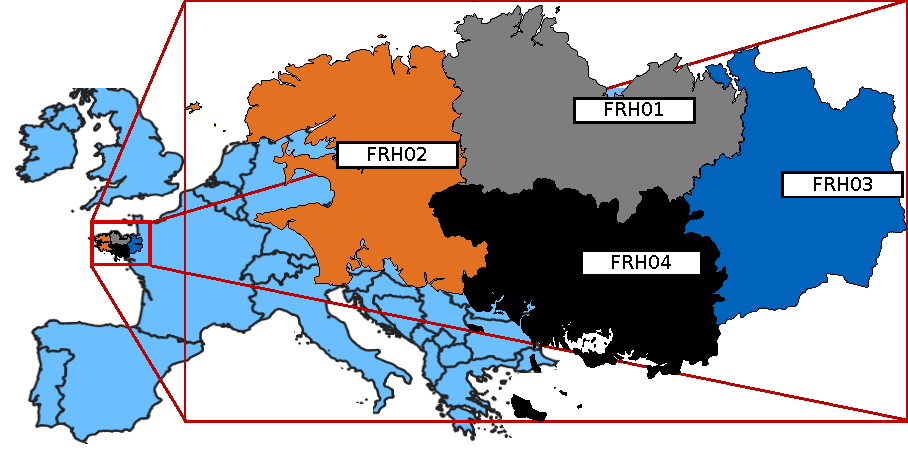
\includegraphics[width=0.9\linewidth]{figures/breizhCrops_regions_black.pdf}
	  \end{minipage}
\end{table}

Table \ref{samples} describes the number of samples per class used for training, validation and test respectively.
It is worth noting that the dataset is highly imbalanced; the most abundant class "temporary meadows has $> 300$ times samples compared to the two minor classes "sunflower" and "nuts". This makes the classification model more sensitive to overfitting and also makes an accuracy evaluation more difficult \cite{Foody2002}. \DIFaddbegin \DIFadd{To ensure perfect comparability with previously published work \mbox{%DIFAUXCMD
\cite{Russwurm2020} }\hskip0pt%DIFAUXCMD
we have chosen to keep the dataset without any modifications.
}\DIFaddend 

\begin{table}[H]
	\centering
	\caption{Number of samples per class used for training, validation and test.}
	\small
	\begin{tabular}{c c c c c}
		\hline
		Class			& Training		& Validation 	& Test 		& Total \\
		\hline
		Barley			& 23,787		& 7,154			& 5,981		& 36,922 \\
		Wheat			& 45,406		& 27,202		& 17,009	& 89,617 \\
		Rapeseed		& 7,945			& 3,557			& 3,244		& 14,746 \\
		Corn			& 80,623		& 42,011		& 31,361	& 153,995 \\
		Sunflower		& 7				& 10			& 2			& 19 \\
		Orchards		& 1,285			& 1,217			& 552		& 3,054 \\
		Nuts			& 28			& 10			& 11		& 49 \\
		Perm. Meadows	& 69,177		& 32,524		& 25,134	& 126,835 \\
		Temp. Meadows	& 91,156		& 52,682		& 38,414	& 182,252 \\
		\hline
	\end{tabular}
	\label{samples}
\end{table}
It is worth mentioning that this dataset provides only spectral signatures in tabular format for the center pixel in a field and not \DIFdelbegin \DIFdel{Sentinel 2 images. 
%DIF <  Nevertheless, to enable our qualitative analysis and produce output classification maps, we downloaded Sentinel 2 images using GEE. However, not all Sentinel 2 products in 2017 are available in GEE database and less images than in Breizhcrops dataset were used for this experiment.
}\DIFdelend \DIFaddbegin \DIFadd{Sentinel-2 images. 
%DIF >  Nevertheless, to enable our qualitative analysis and produce output classification maps, we downloaded Sentinel-2 images using GEE. However, not all Sentinel-2 products in 2017 are available in GEE database and less images than in Breizhcrops dataset were used for this experiment.
}\DIFaddend \subsection{\ac{AEs} training}
With the aim of developing an algorithm capable to process relatively large geographic areas, the \DIFdelbegin \DIFdel{AE is }\DIFdelend \DIFaddbegin \acp{AE}\DIFadd{s are }\DIFaddend composed by a \DIFdelbegin \DIFdel{single layer }\DIFdelend \DIFaddbegin \DIFadd{single-layer }\DIFaddend \ac{FCN} as encoder, and its counterpart for the decoder.
\DIFdelbegin \DIFdel{This keeps computational load and processing times lower than other models}\DIFdelend \DIFaddbegin \DIFadd{While other models, }\DIFaddend such as convolutional \DIFdelbegin \DIFdel{or recurrent networks.
Batch }\DIFdelend \DIFaddbegin \DIFadd{and recurrent networks, require a relatively large number of trainable parameters, as described in \mbox{%DIFAUXCMD
\cite{Paris2020,Chen2022,Russwurm2020}}\hskip0pt%DIFAUXCMD
, the single layer }\acp{AE}\DIFadd{s that form our model need considerably fewer units, meaning lower computational load and faster processing times.
%DIF >  This keeps computational load and processing times lower than other models such as convolutional or recurrent networks.
}

\DIFadd{The batch }\DIFaddend size, learning rate, number of units in \DIFdelbegin \DIFdel{hidden layer and the }\DIFdelend \DIFaddbegin \DIFadd{the hidden layer, and }\DIFaddend loss function were set in accordance with the results acquired through the hyperparameter random search presented in Appendix \ref{app_a}.
The split of the dataset is described in Table \ref{data_split}, which outlines the features employed in this experiment. These include \ac{DOY} (sine and cosine), 10 spectral bands (10 and 20 meters resampled to 10m) and five well-known spectral indices\DIFdelbegin \DIFdel{(}%DIFDELCMD < \ac{NDWI}%%%
\DIFdel{, }%DIFDELCMD < \ac{NDVI}%%%
\DIFdel{, }%DIFDELCMD < \ac{NDTI}%%%
\DIFdel{, }%DIFDELCMD < \ac{NDSVI} %%%
\DIFdel{and }%DIFDELCMD < \ac{EVI}%%%
\DIFdelend \DIFaddbegin \DIFadd{: Normalized difference water index (NDWI), Normalized difference vegetation index (NDVI), Normalized difference tillage index (NDTI), Normalized difference of senescent vegetation index (NDSVI) and Enhanced vegetation index (EVI}\DIFaddend ). Table \ref{hyperparameters_aes} presents the \ac{AEs} configuration.

% \begin{minipage}[t]{0.5\textwidth}
% 	\begin{table}[H]
% 		\caption{Training, validation and testing split, and number of input features and classes considered for the AEs models.}
% 		\begin{tabular}{c|c} 
% 			\hline
% 			Parameter & Value \\ [1ex] 
% 			\hline
% 			Training size & 319,414 \\ [1ex]
% 			Validation size & 166,367 \\[1ex]
% 			Testing size & 122,708 \\ [1ex]
% 			Features & \makecell{10 bands, \\ 2 DOY,\\ 5 spectral indices} \\ [1ex] 
% 			Classes & 9 \\ [1ex] 
% 			\hline
% 		\end{tabular}
% 	\label{data_split}
% 	\end{table}
% \end{minipage}
% \begin{minipage}[t]{0.35\textwidth}
% 	\begin{table}[H]
% 		\caption{AEs hyperparameters final configuration established by random search.}
% 		\begin{tabular}{c|c}
% 		\hline
% 			\multicolumn{2}{c}{Hyperparameters} \\ \hline
% 			Epochs & 1000 \\
% 			Early stop & True \\ 
% 			Patience & 10 \\ 
% 			Min. delta & 1e-5 \\ 
% 			Batch size rate & 0.05* \\ 
% 			Units in hidden layers & 5 \\ 
% 			Learning rate & 1e-4 \\ 
% 			Optimizer & Adam \\ 
% 			Loss & MSE \\ \hline
% 			\multicolumn{2}{c}{* proportion of samples for each class}
% 		\end{tabular}
% 		\label{hyperparameters_aes}
% 	\end{table}
% \end{minipage}

\begin{minipage}[t]{0.45\textwidth}
	\begin{table}[H]
        \centering
        \footnotesize
		\caption{Training, validation and testing split, and number of input features and classes considered for the autoencoders.}
		\begin{tabular}{c|c} 
			\hline
			Parameter & Value \\ [1ex] 
			\hline
			Training size & 319,414 \\ [1ex]
			Validation size & 166,367 \\[1ex]
			Testing size & 122,708 \\ [1ex]
			Features & \makecell{10 bands, \\ 2 DOY,\\ 5 spectral indices} \\ [1ex] 
			Classes & 9 \\ [1ex] 
			\hline
		\end{tabular}
	\label{data_split}
	\end{table}
\end{minipage}\hspace{0.5cm}
\begin{minipage}[t]{0.45\textwidth}
	\begin{table}[H]
        \centering
        \footnotesize
		\caption{Autoencoders (AEs) hyperparameters final configuration established by random search.}
		\begin{tabular}{c|c}
		\hline
			Hyperparameter & Value \\ \hline
			Epochs & 10000 \\
			Early stop & True \\ 
			Patience & 10 \\ 
			Min. delta & 1e-5 \\ 
			Batch size rate & 0.05* \\ 
			Units in hidden layers & 5 \\ 
			Learning rate & 1e-4 \\ 
			Optimizer & Adam \\ 
			Loss & MSE \\ \hline
			\multicolumn{2}{c}{* proportion of samples for each class}
		\end{tabular}
		\label{hyperparameters_aes}
	\end{table}
\end{minipage}\vspace{0.5cm}

% \subsection{Loss functions}
% Considering the regression loss functions Mean Absolute Error (MAE) and Mean Square Error (MSE) as the search elements in our random search, MAE is defined by
% as the loss function for this experiments, since it performed slightly better than mse in most of the runs.
% Figure \ref{loss_fuctions} shows, for each AE, the training and validation loss function computed as the mean absolute error (MAE)
% \begin{equation}
% 	MAE = \frac{1}{M}\sum_{m=0}^{M}|x_m - \hat{x}_m|
% \end{equation}

% Figure \ref{loss_fuctions} shows, for each AE, the training and validation loss function computed as the Mean Squared Error (MSE)
% \begin{equation}
% 	\ac{MSE}=\frac{1}{N} \sum_{n=1}^{N} (\mathbf{y}_{n} - \hat{\mathbf{y}}_{n})^{2}
% \end{equation}

% We can see a soft MAE decrease, both for the training (blue) and validation (orange) data. In some AEs (\ref{fig:loss_nuts}, \ref{fig:loss_sunflower}, \ref{fig:loss_orchards}), the loss function still decays at the last epoch, but was stopped according to our hyperparameters setting \ref{hyperparameters_aes}.
% \begin{figure}[H]
% 	\begin{subfigure}[t]{0.3\textwidth}
% 		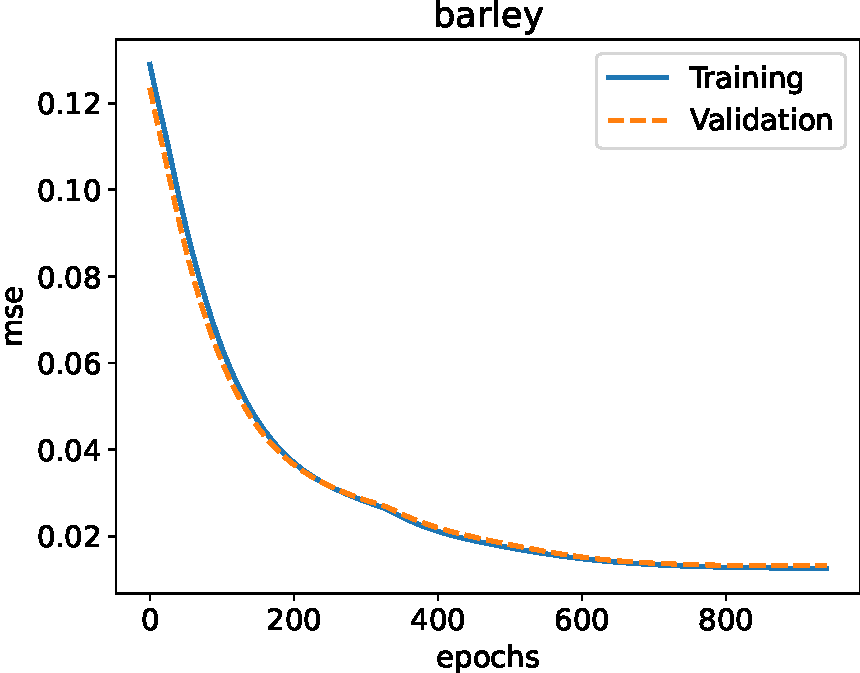
\includegraphics[width=\linewidth]{figures/aes_1_layer_mse_results/loss_functions/loss_barley.pdf}
% 	\caption{}
% 	\label{fig:loss_barley}
% 	\end{subfigure}\hfill
% 	\begin{subfigure}[t]{0.3\textwidth}
% 	  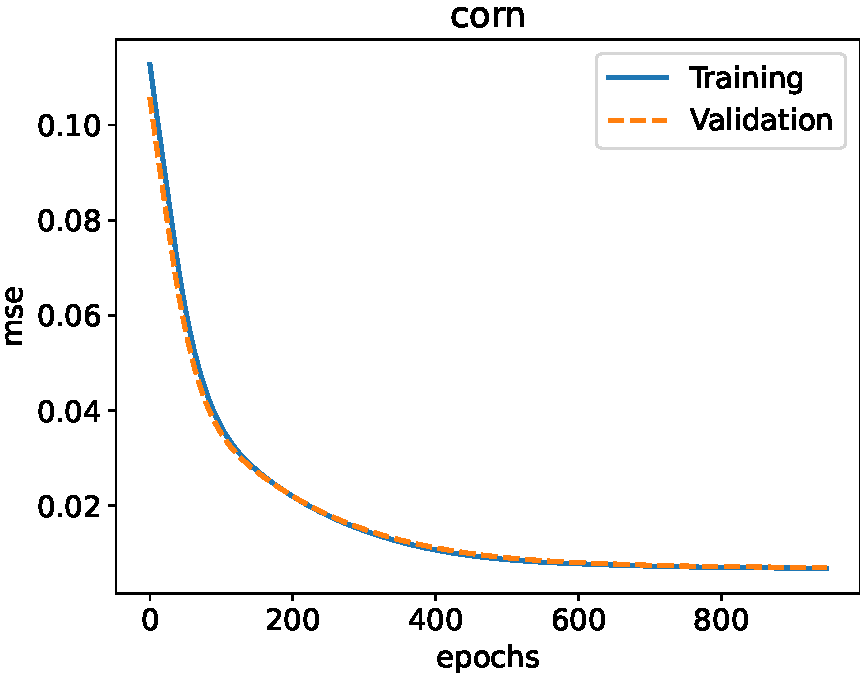
\includegraphics[width=\linewidth]{figures/aes_1_layer_mse_results/loss_functions/loss_corn.pdf}
% 	\caption{}
% 	\label{fig:loss_corn}
% 	\end{subfigure}\hfill
% 	\begin{subfigure}[t]{0.3\textwidth}
% 		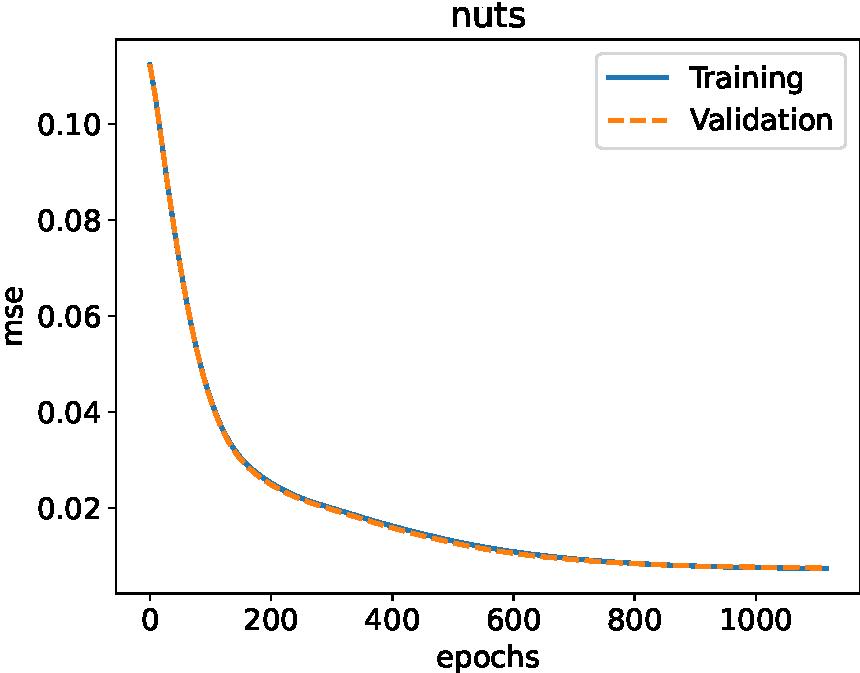
\includegraphics[width=\linewidth]{figures/aes_1_layer_mse_results/loss_functions/loss_nuts.pdf}
% 	\caption{}
% 	\label{fig:loss_nuts}
% 	\end{subfigure}\\[0.2cm]
% 	\begin{subfigure}[t]{0.3\textwidth}
% 		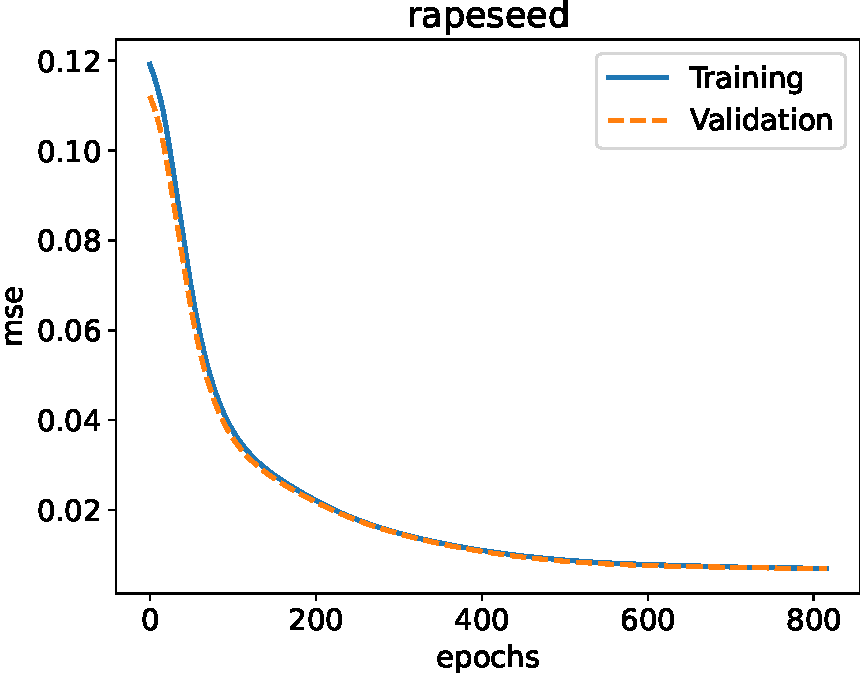
\includegraphics[width=\linewidth]{figures/aes_1_layer_mse_results/loss_functions/loss_rapeseed.pdf}
% 	\caption{}
% 	\label{fig:loss_rapeseed}
% 	\end{subfigure}\hfill
% 	\begin{subfigure}[t]{0.3\textwidth}
% 		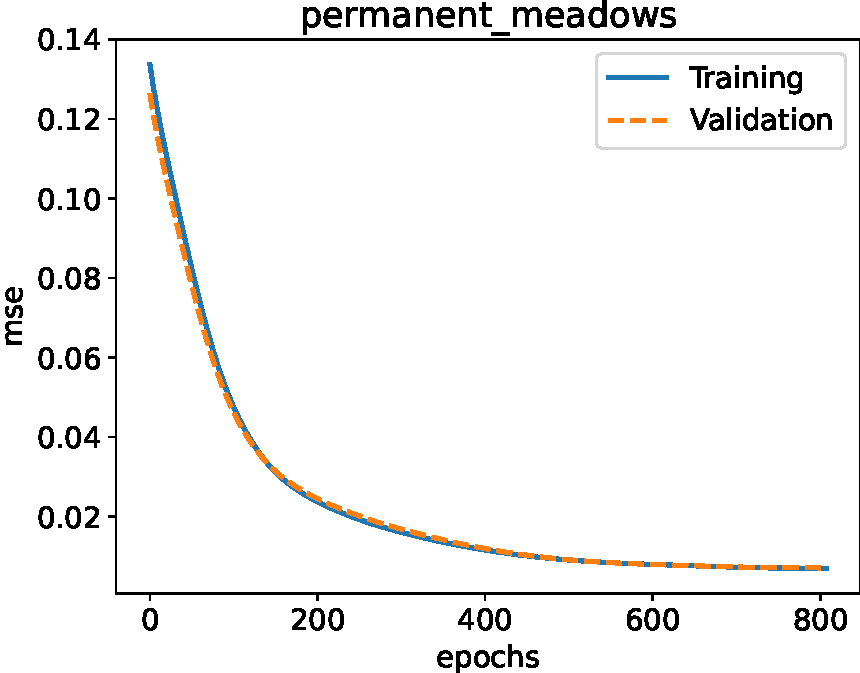
\includegraphics[width=\linewidth]{figures/aes_1_layer_mse_results/loss_functions/loss_permanent_meadows.pdf}
% 	\caption{}
% 	\label{fig:loss_pm}
% 	\end{subfigure}\hfill
% 	\begin{subfigure}[t]{0.3\textwidth}
% 		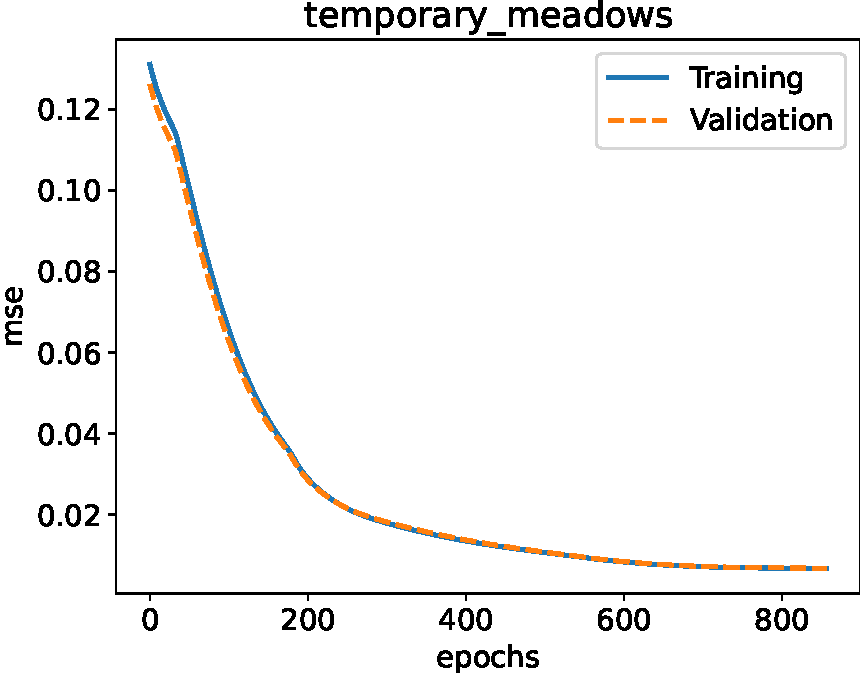
\includegraphics[width=\textwidth]{figures/aes_1_layer_mse_results/loss_functions/loss_temporary_meadows.pdf}
% 	\caption{}
% 	\label{fig:loss_tm}
% 	\end{subfigure}\\[0.2cm]
% 	\begin{subfigure}[t]{0.3\textwidth}
% 		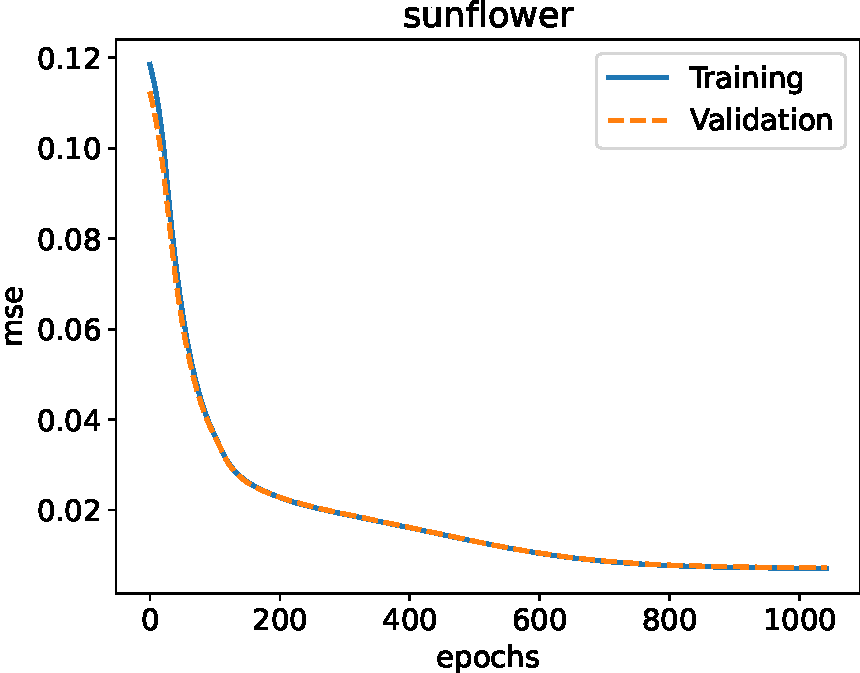
\includegraphics[width=\linewidth]{figures/aes_1_layer_mse_results/loss_functions/loss_sunflower.pdf}
% 	\caption{}
% 	\label{fig:loss_sunflower}
% 	\end{subfigure}\hfill
% 	\begin{subfigure}[t]{0.3\textwidth}
% 		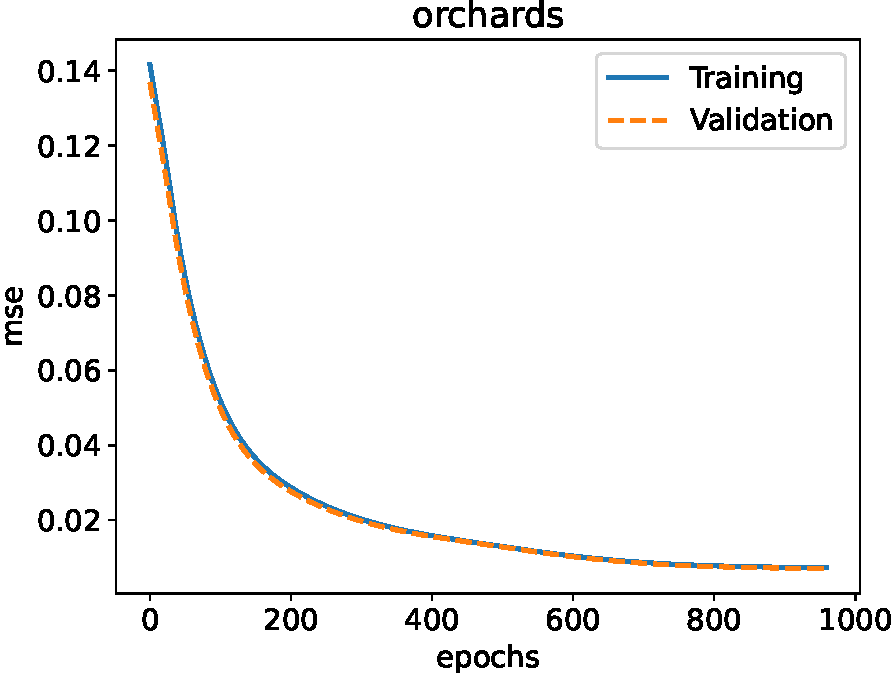
\includegraphics[width=\linewidth]{figures/aes_1_layer_mse_results/loss_functions/loss_orchards.pdf}
% 	\caption{}
% 	\label{fig:loss_orchards}
% 	\end{subfigure}\hfill
% 	\begin{subfigure}[t]{0.3\textwidth}
% 		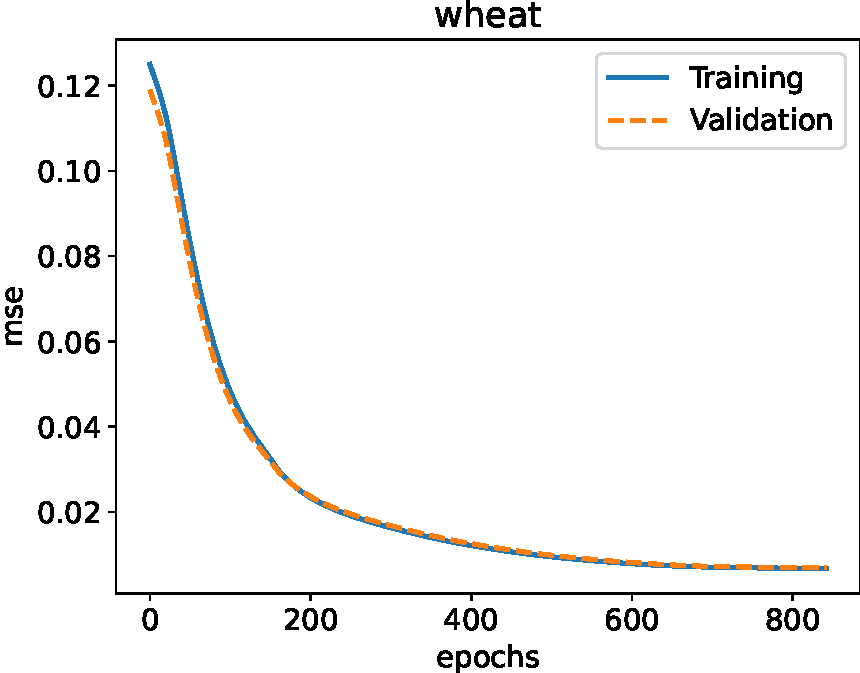
\includegraphics[width=\linewidth]{figures/aes_1_layer_mse_results/loss_functions/loss_wheat.pdf}
% 	\caption{}
% 	\label{fig:loss_wheat}
% 	\end{subfigure}
% 	\caption{Loss functions of AEs trained with (a) barley, (b) corn, (c) nuts, (d) rapeseed, (e) permanent meadows, (f) temporary meadows, (g) sunflower (h) orchards and (i) wheat samples.}
% 	\label{loss_fuctions}
% \end{figure}

\subsection{Separability assessment and distance metrics}
For qualitative assessment of the inter-class separability in the generated representation space, 3D scatterplots of the test spectral-temporal Sentinel-2 \ac{BOA} data and their corresponding representations produced by our method, reduced to a three-dimensional space by t-distributed Stochastic Neighbor Embedding (TSNE), are shown in Figures \ref{fig:pca_raw} and \ref{fig:pca_rep} respectively.
The \DIFdelbegin \DIFdel{scatter plot of representations, compared with that of the initial data, shows }\DIFdelend \DIFaddbegin \DIFadd{figures show }\DIFaddend that the density of points belonging to each of the crop types is much better clustered.
\begin{figure}[H]
	\centering
	\begin{subfigure}[t]{0.35\linewidth}
		\centering
		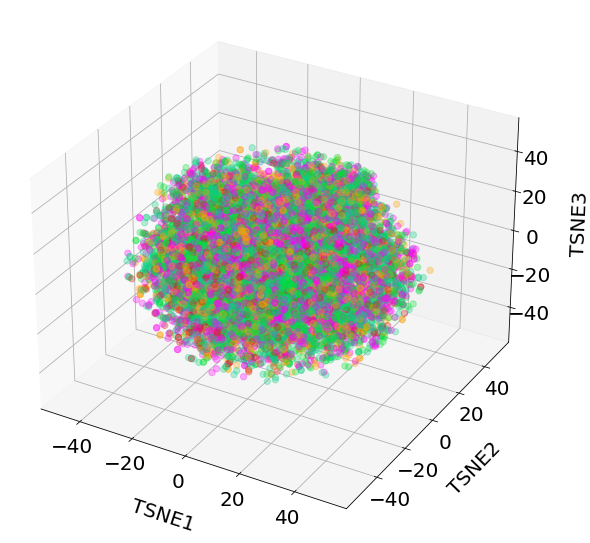
\includegraphics[width=0.9\linewidth]{figures/aes_1_layer_mse_results/s2_TSNE_v3.png}
		\caption{}
	  \label{fig:pca_raw}
	\end{subfigure}
	\begin{subfigure}[t]{0.35\linewidth}
		\centering
		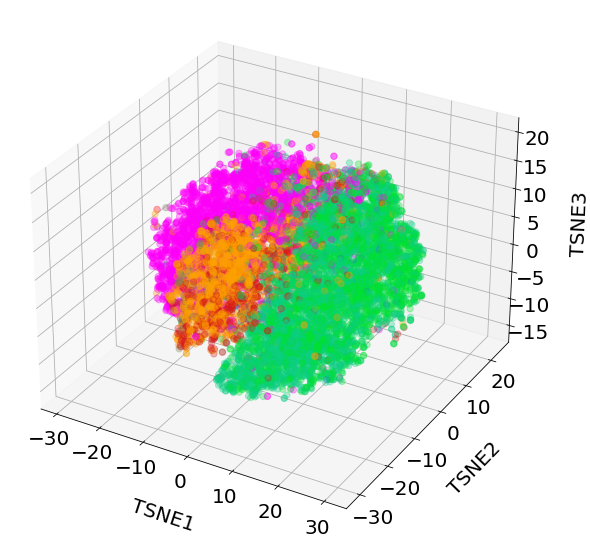
\includegraphics[width=0.9\linewidth]{figures/aes_1_layer_mse_results/representations_TSNE_v5.png}
	\caption{}
	\label{fig:pca_rep}
	\end{subfigure}
     \begin{subfigure}[t]{0.15\linewidth}
        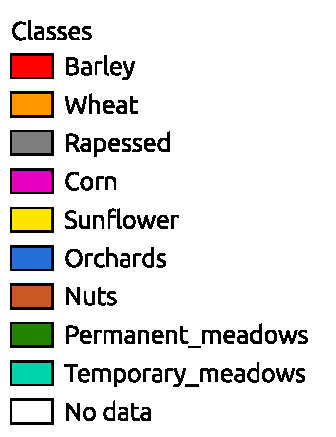
\includegraphics[width=\textwidth]{figures/aes_1_layer_mse_results/labels.pdf}
    \end{subfigure}
	\caption{3D-scatterplot of (a) S2 fixed-length time series (45 observations) and (b) representation, over three principal components obtained by t-distributed Stochastic Neighbor Embedding (TSNE) only for visual interpretation.}
	\label{fcn_losses}
\end{figure}
% \begin{figure}[H]
% 	\centering
% 	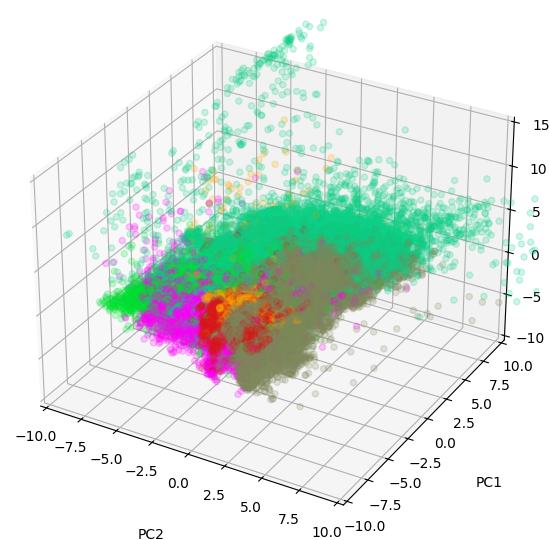
\includegraphics[width=0.4\linewidth]{figures/PCA_3D.png}
% 	\caption{Representation over three principal components obtained by PCA applied to the reconstruction difference of the AEs.}
% 	\label{fig:pca}
% Several distance metrics were used to assess the distance between classes. Table \ref{distance_metrics_results} presents a comparison of the inter-class separability on the input spectral-temporal data and the generated representations, measured by Silhouette score ($SS$) ranges from -1 for incorrect clustering and +1 for highly dense clustering, Calinski-harabasz index ($CH$) larger scores indicates better separability, Davies-bouldin index ($DBI$) ranges from 0 to $\infty$ and the closer to zero the better partition. In addition, we used K-means algorithm to find the clusters centroids and compute the commonly used euclidean distance ($ED$), mahalanobis distance ($MD$) and manhattan distance ($M$) larger scores indicates better separability.
% % silhouette score (SS), calinski-harabasz index (CH), davies-douldin index (DBI). In addition, we used K-means algorithm to find the clusters centroids and compute the commonly used euclidean distance (ED), mahalanobis distance (MD) and manhattan distance (M) (see Appendix \ref{app_distance_m} for metrics definitions).
% In the same way as in the qualitative analysis, distance scores demonstrate much higher separability on the representation space than on the initial data.
% \begin{table}[H]
% 	\centering
% 	\caption{Class distance assessment of the S2 dataset and the representations produced by our method. Silhouette score ($SS$), Calinski-harabasz index ($CH$), Davies-bouldin index ($DBI$). For clusters centroids distance assessment, euclidean distance ($ED$), mahalanobis distance ($MD$) and manhattan distance ($M$).}
% 	\begin{tabular}{c|c|c}
% 		\hline
% 		Distance metric & S2 & Our approach \\
% 		\hline  	
% 		$SS$ & -0.76 & \textbf{0.20} \\
%         $CH$ & 1.4 & \textbf{73074.46} \\
% 		$DBI$ & 72.44  & \textbf{18.96} \\ 
%         \hline
%         $ED$ & 0.3205 & \textbf{0.6665}\\
%         $MD$ & 2.2907 & \textbf{2.3545}\\
%         $M$ & 0.4688& \textbf{0.9725}\\
% 		\hline
% 	\end{tabular}
% 	\label{distance_metrics_results}
% \end{table}

Several distance metrics were used to \DIFdelbegin \DIFdel{assess }\DIFdelend \DIFaddbegin \DIFadd{quantify }\DIFaddend the distance between classes. Table \ref{distance_metrics_results} presents a comparison of the inter-class separability on the input spectral-temporal Sentinel-2 BOA data and the generated representations, measured by: Silhouette score ($SS$), which ranges from -1 for incorrect clustering and +1 for highly dense clustering, Calinski-Harabasz index ($CH$), for which larger scores indicates better separability, and Davies-Bouldin index ($DBI$), which ranges from 0 to $\infty$ and the closer to zero the better the separability between clusters (see Appendix \ref{app_distance_m} for metrics definitions).
% silhouette score (SS), calinski-harabasz index (CH), davies-douldin index (DBI). In addition, we used K-means algorithm to find the clusters centroids and compute the commonly used euclidean distance (ED), mahalanobis distance (MD) and manhattan distance (M) (see Appendix \ref{app_distance_m} for metrics definitions).

\DIFdelbegin \DIFdel{In the same way as in the qualitative analysis, distance scores }\DIFdelend \DIFaddbegin \DIFadd{The distance scores again }\DIFaddend demonstrate much higher separability \DIFdelbegin \DIFdel{on }\DIFdelend \DIFaddbegin \DIFadd{in }\DIFaddend the representation space than on the initial data.
\begin{table}[H]
	\centering
	\caption{Class distance assessment of the S2 dataset and the representations produced by our method. Silhouette score ($SS$), Calinski-Harabasz index ($CH$), Davies-Bouldin index ($DBI$).}
	\begin{tabular}{c|c|c}
		\hline
		Distance metric & S2 data & Our approach \\
		\hline  	
		$SS$ & -0.76 & \textbf{0.20} \\
        $CH$ & 1.4 & \textbf{73074.46} \\
		$DBI$ & 72.44  & \textbf{18.96} \\ 
		\hline
	\end{tabular}
	\label{distance_metrics_results}
\end{table}

\subsection{Evaluating representations in the classification of crop types}\label{results_section}
% Class separability and classification metrics are used in this work to assess the quality of the derived representations.
%Different quality indicators can be considered for representations assessment. For the particular case of representations for classification, class separability and classification metrics are used in this work.
% For evaluating the representations, there are different methods like clustering, distance metrics \cite{Shutaywi2021}, rankme \cite{Garrido2023, Balestriero2023}, . We 
% \cite{Garrido2023}

% \subsubsection{Fully conected network classifier}

% We decided to use a fully conected network as the classification model, 
% where the input are the representations with their correspond label. 
% In this part, it is important to note that the dataset is imbalanced, 
% i.e., all the classes have a different number of samples, which makes the classification model more sensitive to overfitting. 
% The description of the classifier is described in the Table \ref{fcn_hyperparameters}.
Once the representations have been produced, a 3-layer FCN was used as classification model, where the inputs are the generated representations and their corresponding labels. The parameters of the classifier are detailed in Table \ref{fcn_hyperparameters}.
\DIFdelbegin \DIFdel{The elements corresponding to the differences in the }%DIFDELCMD < \ac{DOY} %%%
\DIFdel{embeddings are not considered as part of the final representation vectors, since averaging these elements induces redundancy to the classification model. Hence, }\DIFdelend %DIF >  The elements corresponding to the differences in the \ac{DOY} embeddings are not considered as part of the final representation vectors, since averaging these elements induces redundancy to the classification model. 
\DIFaddbegin \DIFadd{Note that }\DIFaddend the input dimensionality is defined by $B$ spectral bands plus 5 spectral indices times $C$ number of AEs\DIFaddbegin \DIFadd{, as the DOY embeddings would induce redundancy}\DIFaddend .
\begin{table}[H]
	\centering
	\caption{Classification model configuration.}
 	% \caption{Classification model hyperparameters. $B$ denotes the number of bands, and $C$ the number of autoencoders (AEs). Note that only 5 additional features (the spectral vegetation indices) are added to the spectral bands, since day-of-Year (DOY) features are excluded from the representations in the training of the classification model.}
	\begin{tabular}{c|c}
	\hline
		Hyperparameter & Value \\ \hline
		Input size & $(B + 5) \times C = 135$ \\
		Epochs & 10000 \\ 
		% Patience & 100 \\ 
		% Min. delta & 1e-5 \\ 
		Batch size & 1000\\ 
        %Scaler & MinMax \\
		Units in hidden layers & 128, 64, 32 \\  
		Learning rate & 1e-4 \\
		Optimizer & Adam \\ 
		Loss & Categorical crossentropy \\ \hline
	\end{tabular}
	\label{fcn_hyperparameters}
\end{table}

% \subsubsection{Confusion matrix}
% In the figure \ref{confusion_matrix} we can see the confusion matrix where, it shows the results of the fcn classifier. 
% In the principal diagonal you can see the samples were classified sucessfull and out of it the samples misclassified.

% \begin{figure}[H]
% 	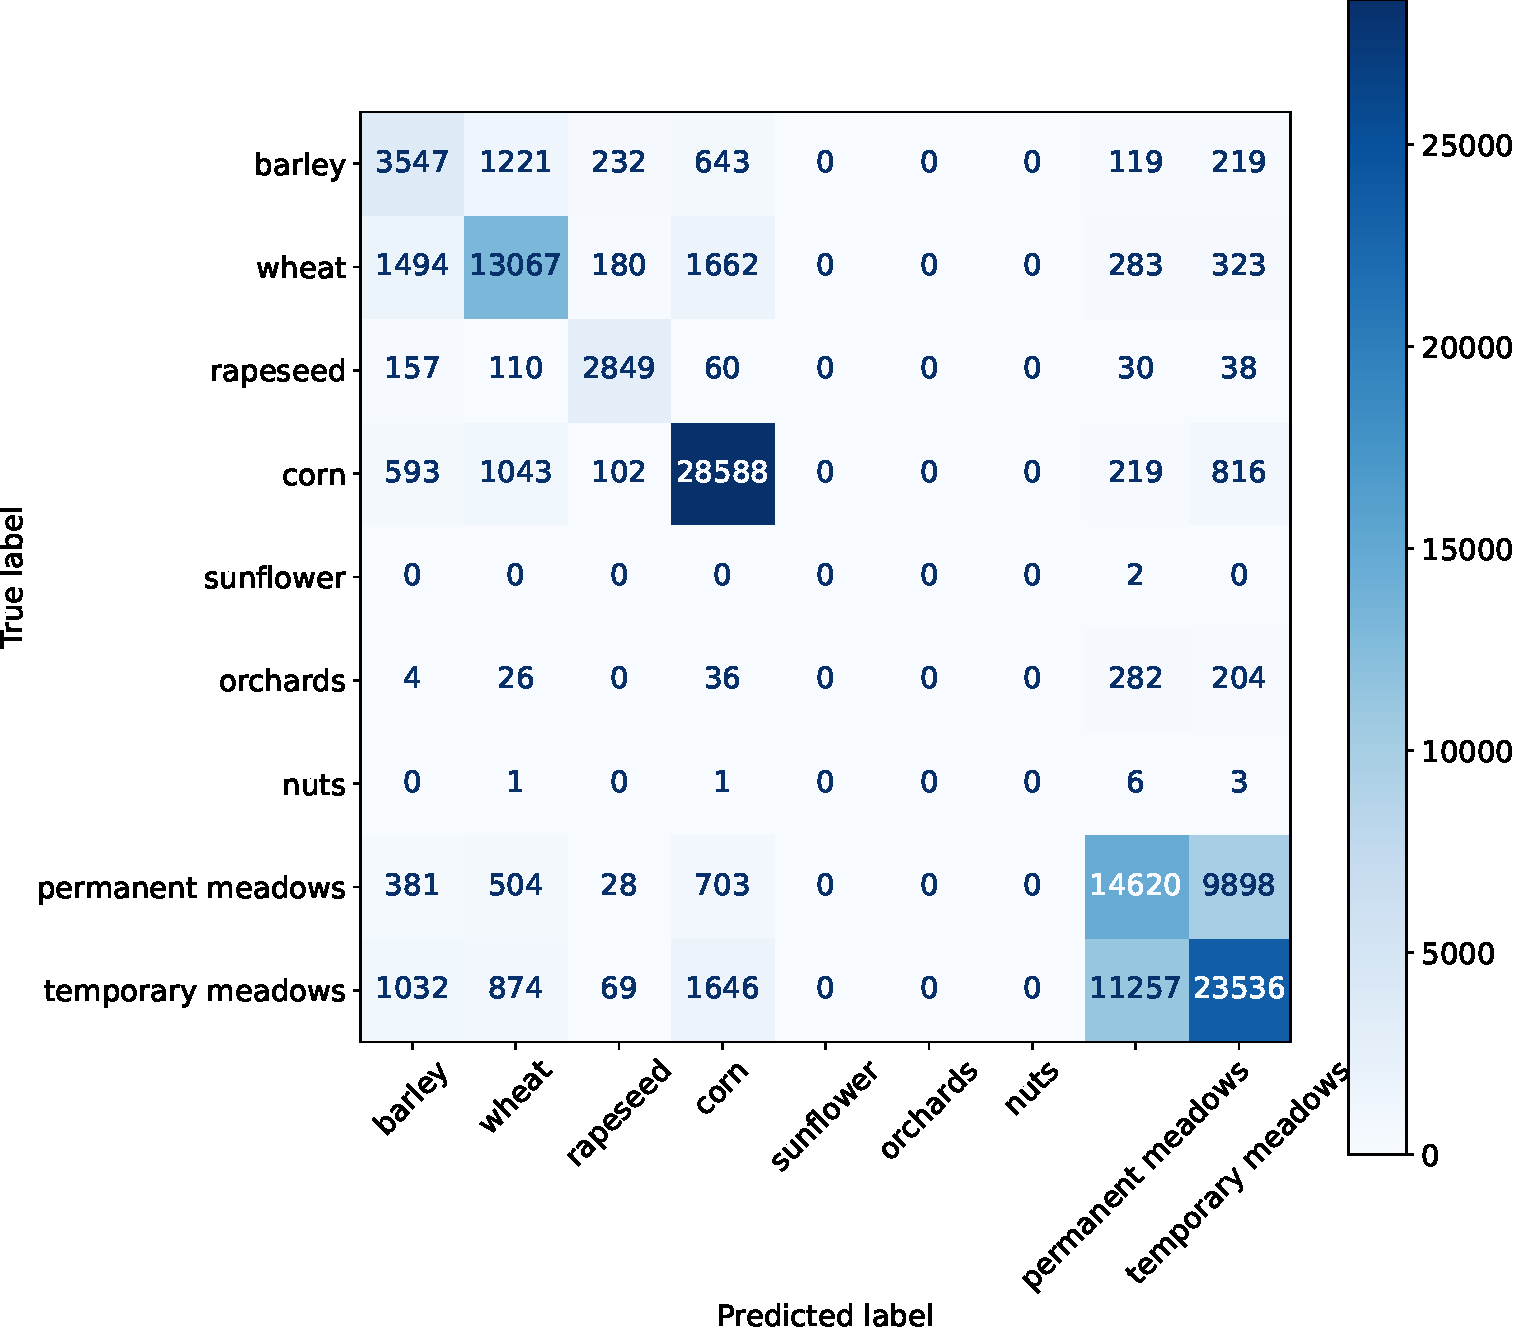
\includegraphics[width=.7\textwidth]{figures/confusion_matrix_test.pdf}
% 	\caption{Confusion matrix of the FCN prediction for the testing data.}
% 	\label{confusion_matrix}
% \end{figure}


% \subsection{Results}
% In this section, quantitative results of the proposed framework are presented and compared with results reported in \cite{Russwurm2020} for different state of the art methods. 
% For qualitative interpretation, classification maps are shown using the obtained representations.

% % \subsubsection{Quantitative results}
% In addition to monitoring training and validation loss functions, the overall accuracy (OA) is monitored as indicator of classification model performance. Due to the clear imbalance among classes, BreizhCrops is an extremely challenging dataset. Therefore, the Matthews correlation coefficient (MCC), which is robust to class imbalance, is also monitored for a less biased evaluation. Figure \ref{fcn_losses} presents the progress of these metrics during model fitting.
% In Figure \ref{fig:fcn_loss} MSE on validation dataset follows the same descending trend as in the training dataset, indicating that no overfitting occurs during training. From Figures \ref{fig:fcn_accuracy} and \ref{fig:fcn_mcc}, it can be seen that OA and MCC are slightly better on the training dataset.
% % The loss function is still decreasing for training but not for validation in Figure \ref{fig:fcn_loss}. 
% % The overall accuracy of the Figure \ref{fig:fcn_accuracy} is still increasing to an acceptable level.
% % The imbalance in the dataset led to the consideration of the MCC metric (see Figure \ref{fig:fcn_mcc}).
% \begin{figure}[H]
% 	\centering
% 	\begin{subfigure}[t]{0.3\linewidth}
% 		\centering
% 		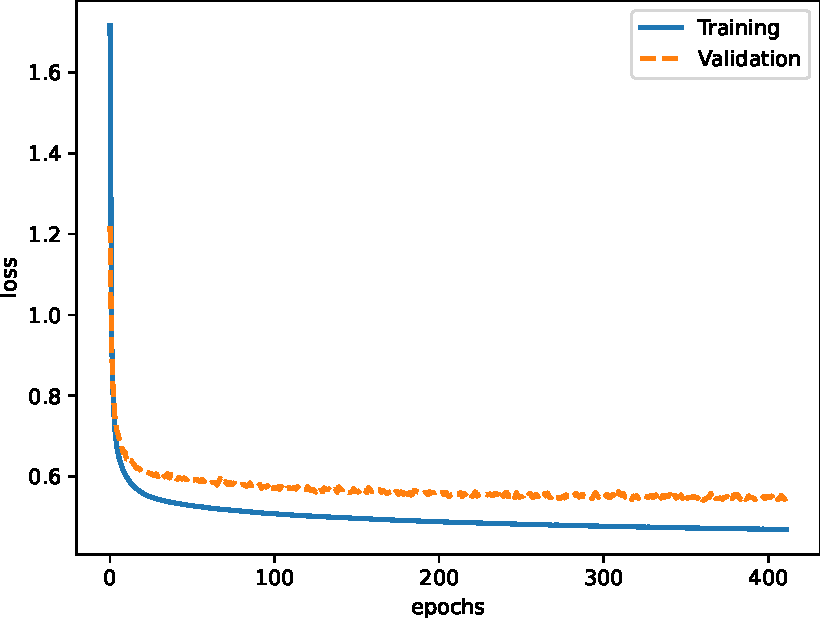
\includegraphics[width=\linewidth]{figures/aes_1_layer_mse_results/fcn_loss.pdf}
% 	  \caption{}
% 	  \label{fig:fcn_loss}
% 	\end{subfigure}
% 	\begin{subfigure}[t]{0.3\linewidth}
% 		\centering
% 		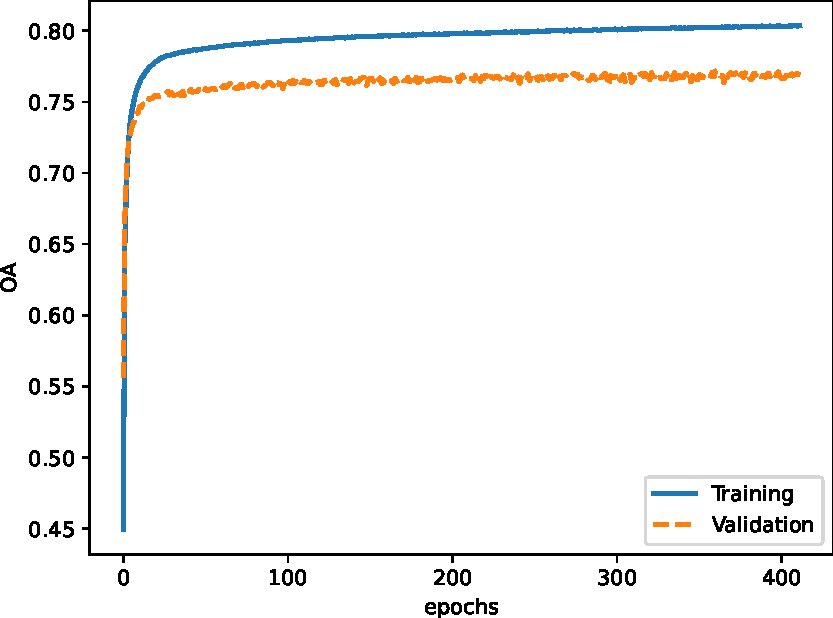
\includegraphics[width=\linewidth]{figures/aes_1_layer_mse_results/fcn_accuracy.pdf}
% 	\caption{}
% 	\label{fig:fcn_accuracy}
% 	\end{subfigure}
% 	\begin{subfigure}[t]{0.3\linewidth}
% 		\centering
% 		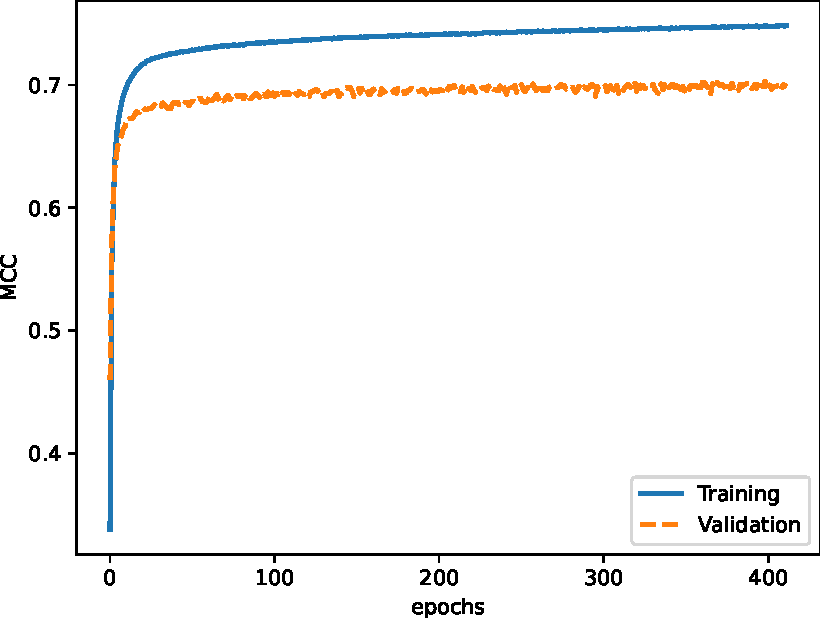
\includegraphics[width=\linewidth]{figures/aes_1_layer_mse_results/fcn_mcc.pdf}
%     \caption{}
% 	\label{fig:fcn_mcc}
% 	\end{subfigure}
% 	\caption{FCN training and validation (a) MSE (b) OA and (c) MCC functions over epochs.}
% 	\label{fcn_losses}
% \end{figure}

% Table \ref{Classification_performance_evaluation_conventional_classifiers} shows the performance evaluation of different traditional classifiers, such as RF, SVM, XGBoost, and FCN, are evaluated by OA, Cohen’s kappa coefficient ($\kappa$) and  MCC, using two types of input data: L2A and Representations. Using Representations gives the RF classifier an OA of 0.73, which is greater than the 0.71 obtained using L2A data. Similarly, the SVM classifier gets an OA of 0.74 using Representations, which exceeds the 0.70 attained with L2A data. XGBoost likewise performs better with Representations 0.71 than with L2A data 0.70 in OA.
% The FCN classifier achieves the best results with both input types but stands out particularly with using the Representations as an input, reaching the highest OA of 0.76. This demonstrates the overall superiority of Representations as input data for improving classification performance across conventional models.\\
% Using the Representations, the $\kappa$ scores are consistently higher across all classifiers than with the L2A data, reflecting improved classification. RF reaches 0.64, SVM achieves 0.66, and XGBoost improves to 0.62. The FCN classifier obtains the highest $\kappa$ value 0.69, showing the best agreement between predicted and true labels. FCN has the greatest MCC (0.69) when using Representations, followed by SVM (0.67) and RF (0.64). The greater MCC for FCN (and other classifiers) when Representations are used illustrates their efficacy in enhancing classification performance.

A comparative study is presented in Table \ref{Classification_performance_evaluation_conventional_classifiers} where the performance of different traditional classifiers, such as RF, SVM, XGBoost, and FCN, are evaluated using two types of input data: fixed length Sentinel-2 BOA data and our derived representations. The evaluation is based on overall accuracy (OA), Cohen's kappa coefficient ($\kappa$) and Matthews correlation coefficient (MCC). All models are tested with exactly the same training and testing samples of the BreizhCrops dataset (as described in Table \ref{samples}) allowing a direct comparison of results. 

In all cases, our representations improved classification performance compared to the use of the original Sentinel-2 data.
Improvement ranged from \DIFdelbegin \DIFdel{$1\%$ to $4\%$ }\DIFdelend \DIFaddbegin \DIFadd{$\sim 2\%$ to $\sim 7\%$ }\DIFaddend in terms of OA. The FCN classifier achieves the best OA, $\kappa$ and MCC with both input types, and stands out particularly using the representations as input, reaching the highest OA=\DIFdelbegin \DIFdel{0.767}\DIFdelend \DIFaddbegin \DIFadd{0.7706}\DIFaddend , $\kappa$=\DIFdelbegin \DIFdel{0.695 }\DIFdelend \DIFaddbegin \DIFadd{0.6995 }\DIFaddend and MCC=\DIFdelbegin \DIFdel{0.698}\DIFdelend \DIFaddbegin \DIFadd{0.7014}\DIFaddend .

% Using the Representations, the $\kappa$ scores are consistently higher across all classifiers than with the L2A data, reflecting improved classification. RF reaches 0.64, SVM achieves 0.66, and XGBoost improves to 0.62. The FCN classifier obtains the highest $\kappa$ value 0.69, showing the best agreement between predicted and true labels. FCN has the greatest MCC (0.69) when using Representations, followed by SVM (0.67) and RF (0.64). 
% This demonstrates the overall superiority of Representations as input data for improving classification performance across conventional models

\begin{table}[H]
    \centering
    \caption{Comparison of classification performance with Sentinel-2 data versus representations produced by our method as input data to conventional classifiers, random forest (RF), support vector machine (SVM), extreme gradient boosting (XGBoost) and fully connected network (FCN) evaluated by overall accuracy (OA), Cohen’s kappa coefficient ($\kappa$), and Matthews correlation coefficient (MCC).}
    \begin{tabular}{c|c c c c| c c c c}
    \hline 
        & \multicolumn{4}{c|}{S2 data} & \multicolumn{4}{c}{Representations}\\ \hline
        Metric &    RF  &   SVM  &   XGBoost &   FCN    &    RF   &   SVM     &   XGBoost &   FCN \\ \hline
         OA   & 0.7172 & 0.7091 &   0.7036  &  0.7438  &  0.7345 &   0.7466  &   0.7139  & \textbf{\DIFdelbeginFL \DIFdelFL{0.7672}\DIFdelendFL \DIFaddbeginFL \DIFaddFL{0.7706}\DIFaddendFL }\\ 
         $\kappa$    & 0.6264 & 0.6197 &   0.6113  &  0.6716  &  0.6464 &   0.6688  &   0.6201  & \textbf{\DIFdelbeginFL \DIFdelFL{0.6953}\DIFdelendFL \DIFaddbeginFL \DIFaddFL{0.6995}\DIFaddendFL }\\ 
         MCC   & 0.6326 & 0.6249 &   0.6149  &  0.6729  &  0.6491 &   0.6710  &   0.6234  & \textbf{\DIFdelbeginFL \DIFdelFL{0.6977}\DIFdelendFL \DIFaddbeginFL \DIFaddFL{0.7014}\DIFaddendFL } \\ \hline
    \end{tabular}
    \label{Classification_performance_evaluation_conventional_classifiers}
\end{table}

We conducted a comparison between representations and S2 data across all classifiers in scenarios with limited labeled data. Results presented in Figure \ref{oa_vs_train_pct} demonstrate that the representations consistently offer greater stability and maintain higher accuracy as the percentage of available training data decreases.

The FCN benefits exceptionally from representations, it obtains the highest \ac{OA} of $\sim 0.77$ using $100 \%$ of the training data, and its classification performance is much less affected compared to the use of the original Sentinel-2 data as the number of training samples decreases. 
% representations allowing FCN to maintain a steadier performance, showing its advantage in low-data scenarios. 
% On the other hand, when the input is S2-BOA data, it starts with accuracy among classifiers, around $\sim 0.74$ at $100 \%$ training data. 
% However, as the training data decreases, FCN's performance significantly drops. For RF, representations are highly effective due to, maintaining an acceptable accuracy even as data availability decreases. 
SVM, in combination with the representations, keeps the classification performance stable, even with very low number of training samples (around 30,000), offering clear improvements over S2 data and making it the best option in this scenario. XGBoost and RF, on the other hand, offer stable performance with S2, but the use of representations considerably elevates accuracy.

% The Figure \ref{oa_vs_train_pct} shows the representations outperform S2-BOA for all classifiers, particularly as the amount of training data decreases. Due to, they are enriched representations improve model robustness and accuracy, especially in data-scarce environments, making the representations the best overall representation across all models.

\begin{figure}[H]
	\centering
	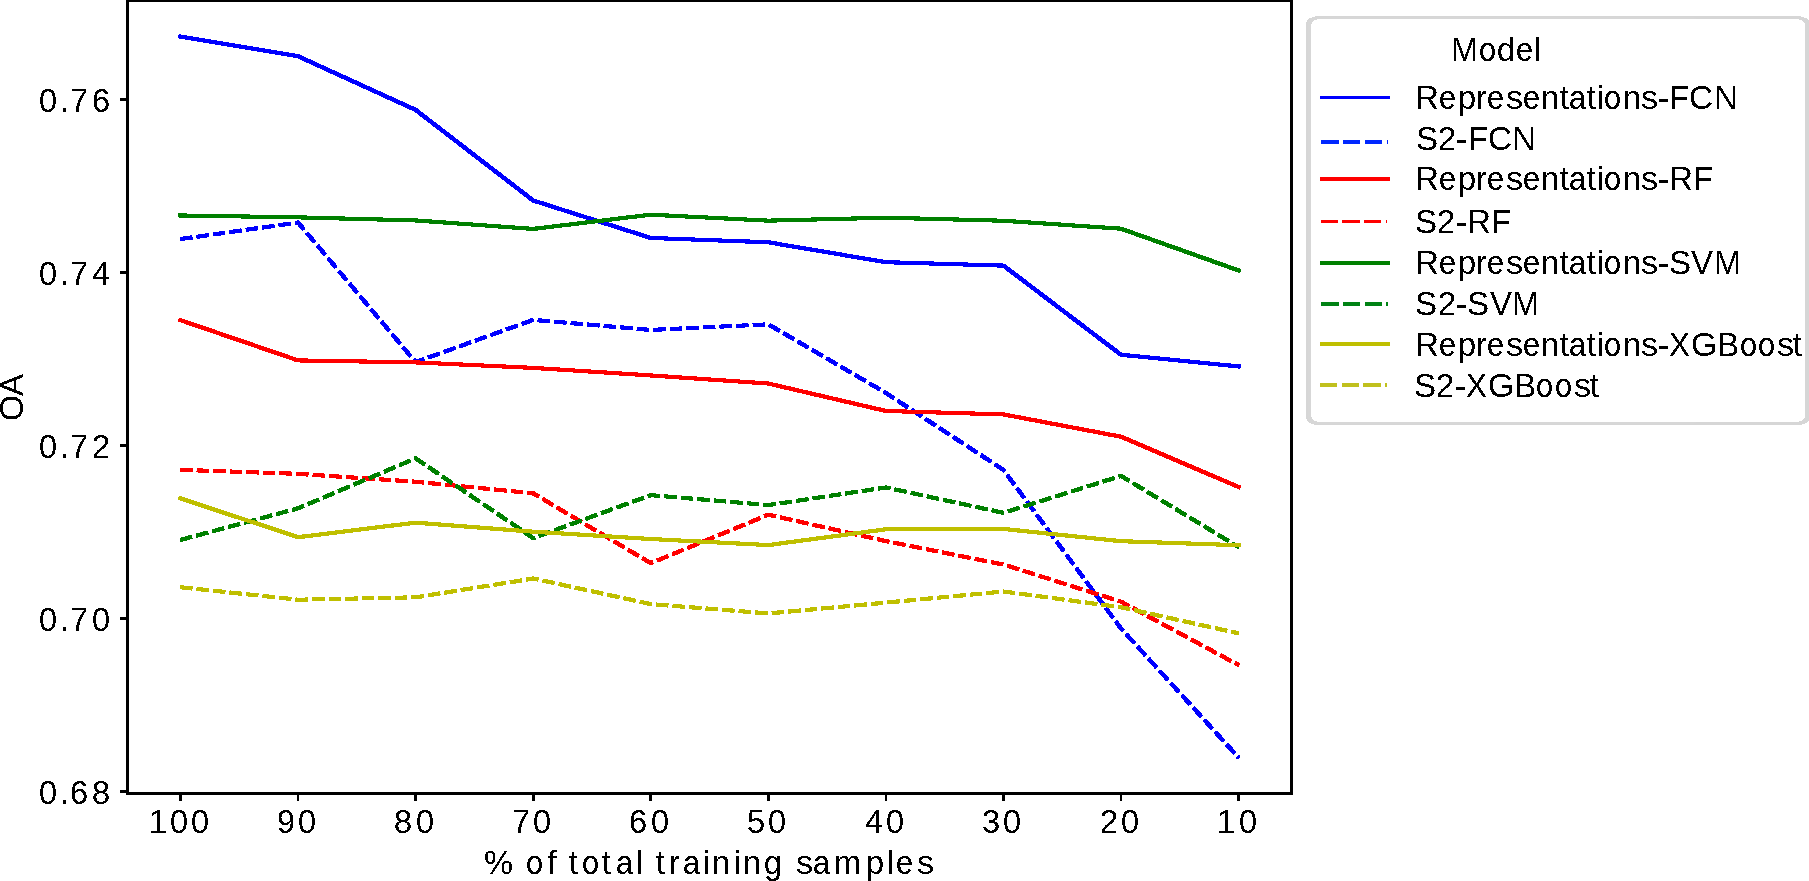
\includegraphics[width=\textwidth]{figures/oa_vs_train_pct_corrected-2.pdf}
	\caption{Overall Accuracy (OA) of random forest (RF), support vector machine (SVM), extreme gradient boosting (XGBoost) and fully connected network (FCN) trained with variable percentage of training samples and using (i) representations (solid line), and (ii) original Sentinel-2 data (broken line).}
	\label{oa_vs_train_pct}    
\end{figure}

The confusion matrix shown in Table \ref{confusion_matrix} presents the model performance on the testing dataset.
Our approach performs relatively accurate for wheat, rapeseed and corn samples, and, although permanent and temporary meadows samples are not accurately classified, both classes are actually the same crop type, and misclassified samples are mainly due to their similar nature as shown in the last two rows of the confusion matrix. However, our approach is inaccurate for the small \DIFdelbegin \DIFdel{and challenging }\DIFdelend classes in this dataset, i.e., sunflower \DIFdelbegin \DIFdel{, orchards and nuts}\DIFdelend \DIFaddbegin \DIFadd{and nuts, which can not be separated due to the very limited samples provided}\DIFaddend . The misclassification of these classes is probably not related to incapacity of the model to deal with imbalanced datasets, but is a direct result of the very limited number of samples\DIFaddbegin \DIFadd{, as was also outlined by the authors in \mbox{%DIFAUXCMD
\cite{Russwurm2020}}\hskip0pt%DIFAUXCMD
. As the spectral signatures provided in the dataset are field-based averages, classes such as orchards, where trees only cover single pixels with large areas between the trees, are easily confused by our model with regular parcels of meadows}\DIFaddend .
\begin{table}[H]
\centering
\scriptsize
\caption{Confusion matrix of the fully connected network (FCN) prediction for the testing data.}
\begin{tabular}{c|ccccccccc}
\hline
\makecell{Object\\based} & Barley & Wheat & Rapeseed & Corn & Sunflower & Orchards & Nuts & \makecell{Permanent\\meadows} & \makecell{Temporary\\meadows} \\ \hline
Barley      & \DIFdelbeginFL \DIFdelFL{4653  }\DIFdelendFL \DIFaddbeginFL \DIFaddFL{4608  }\DIFaddendFL & \DIFdelbeginFL \DIFdelFL{760   }\DIFdelendFL \DIFaddbeginFL \DIFaddFL{642   }\DIFaddendFL & \DIFdelbeginFL \DIFdelFL{40   }\DIFdelendFL \DIFaddbeginFL \DIFaddFL{71   }\DIFaddendFL & \DIFdelbeginFL \DIFdelFL{163   }\DIFdelendFL \DIFaddbeginFL \DIFaddFL{231   }\DIFaddendFL & 0 & 0 & 0 & \DIFdelbeginFL \DIFdelFL{31    }\DIFdelendFL \DIFaddbeginFL \DIFaddFL{29    }\DIFaddendFL & \DIFdelbeginFL \DIFdelFL{334   }\DIFdelendFL \DIFaddbeginFL \DIFaddFL{400   }\DIFaddendFL \\
Wheat       & \DIFdelbeginFL \DIFdelFL{535  }\DIFdelendFL \DIFaddbeginFL \DIFaddFL{626   }\DIFaddendFL & \DIFdelbeginFL \DIFdelFL{15850 }\DIFdelendFL \DIFaddbeginFL \DIFaddFL{15681 }\DIFaddendFL & 14   & \DIFdelbeginFL \DIFdelFL{179   }\DIFdelendFL \DIFaddbeginFL \DIFaddFL{206   }\DIFaddendFL & 0 & 0 & 0 & 79   & \DIFdelbeginFL \DIFdelFL{352   }\DIFdelendFL \DIFaddbeginFL \DIFaddFL{406   }\DIFaddendFL \\
Rapeseed    & \DIFdelbeginFL \DIFdelFL{208   }\DIFdelendFL \DIFaddbeginFL \DIFaddFL{130   }\DIFaddendFL & \DIFdelbeginFL \DIFdelFL{25    }\DIFdelendFL \DIFaddbeginFL \DIFaddFL{17    }\DIFaddendFL & \DIFdelbeginFL \DIFdelFL{2864  }\DIFdelendFL \DIFaddbeginFL \DIFaddFL{2949 }\DIFaddendFL & \DIFdelbeginFL \DIFdelFL{42    }\DIFdelendFL \DIFaddbeginFL \DIFaddFL{31    }\DIFaddendFL & 0 & 0 & 0 & \DIFdelbeginFL \DIFdelFL{13    }\DIFdelendFL \DIFaddbeginFL \DIFaddFL{15    }\DIFaddendFL & \DIFdelbeginFL \DIFdelFL{92   }\DIFdelendFL \DIFaddbeginFL \DIFaddFL{102   }\DIFaddendFL \\
Corn        & \DIFdelbeginFL \DIFdelFL{267   }\DIFdelendFL \DIFaddbeginFL \DIFaddFL{236   }\DIFaddendFL & \DIFdelbeginFL \DIFdelFL{422   }\DIFdelendFL \DIFaddbeginFL \DIFaddFL{314   }\DIFaddendFL & \DIFdelbeginFL \DIFdelFL{22  }\DIFdelendFL \DIFaddbeginFL \DIFaddFL{38   }\DIFaddendFL & \DIFdelbeginFL \DIFdelFL{29547 }\DIFdelendFL \DIFaddbeginFL \DIFaddFL{29900 }\DIFaddendFL & 0 & 0 & 0 & \DIFdelbeginFL \DIFdelFL{104   }\DIFdelendFL \DIFaddbeginFL \DIFaddFL{111   }\DIFaddendFL & \DIFdelbeginFL \DIFdelFL{999  }\DIFdelendFL \DIFaddbeginFL \DIFaddFL{762  }\DIFaddendFL \\
Sunflower   & 0     & 0 & 0 & 0 & 0 & 0 & 0 & 1 & 1 \\
Orchards    & \DIFdelbeginFL \DIFdelFL{3     }%DIFDELCMD < & %%%
\DIFdelFL{6 }%DIFDELCMD < & %%%
\DIFdelendFL 0     & 5 & \DIFaddbeginFL \DIFaddFL{1 }& \DIFaddFL{4 }& \DIFaddendFL 0 & 0 & 0 & \DIFdelbeginFL \DIFdelFL{290   }\DIFdelendFL \DIFaddbeginFL \DIFaddFL{277   }\DIFaddendFL & \DIFdelbeginFL \DIFdelFL{248   }\DIFdelendFL \DIFaddbeginFL \DIFaddFL{265   }\DIFaddendFL \\
Nuts        & 0     & 0 & 0 & 2 & 0 & 0 & 0 & \DIFdelbeginFL \DIFdelFL{5 }\DIFdelendFL \DIFaddbeginFL \DIFaddFL{6 }\DIFaddendFL & \DIFdelbeginFL \DIFdelFL{4 }\DIFdelendFL \DIFaddbeginFL \DIFaddFL{3 }\DIFaddendFL \\
\makecell{Permanent\\meadows}   & \DIFdelbeginFL \DIFdelFL{287   }\DIFdelendFL \DIFaddbeginFL \DIFaddFL{122   }\DIFaddendFL & \DIFdelbeginFL \DIFdelFL{246   }\DIFdelendFL \DIFaddbeginFL \DIFaddFL{212   }\DIFaddendFL & \DIFdelbeginFL \DIFdelFL{14    }\DIFdelendFL \DIFaddbeginFL \DIFaddFL{4    }\DIFaddendFL & \DIFdelbeginFL \DIFdelFL{164   }\DIFdelendFL \DIFaddbeginFL \DIFaddFL{163   }\DIFaddendFL & 0 & 0 & 0 & \DIFdelbeginFL \DIFdelFL{11985 }\DIFdelendFL \DIFaddbeginFL \DIFaddFL{12409 }\DIFaddendFL & \DIFdelbeginFL \DIFdelFL{13438 }\DIFdelendFL \DIFaddbeginFL \DIFaddFL{13224 }\DIFaddendFL \\
\makecell{Temporary\\meadows}   & \DIFdelbeginFL \DIFdelFL{562   }\DIFdelendFL \DIFaddbeginFL \DIFaddFL{451   }\DIFaddendFL & \DIFdelbeginFL \DIFdelFL{439   }\DIFdelendFL \DIFaddbeginFL \DIFaddFL{321   }\DIFaddendFL & \DIFdelbeginFL \DIFdelFL{53    }\DIFdelendFL \DIFaddbeginFL \DIFaddFL{64    }\DIFaddendFL & \DIFdelbeginFL \DIFdelFL{568   }\DIFdelendFL \DIFaddbeginFL \DIFaddFL{628   }\DIFaddendFL & 0 & 0 & 0 & \DIFdelbeginFL \DIFdelFL{7541  }\DIFdelendFL \DIFaddbeginFL \DIFaddFL{7942  }\DIFaddendFL & \DIFdelbeginFL \DIFdelFL{29251 }\DIFdelendFL \DIFaddbeginFL \DIFaddFL{29008 }\DIFaddendFL \\ 
\hline                  
\end{tabular}
\label{confusion_matrix}
\end{table}
% \begin{figure}[H]
% 	\centering
% 	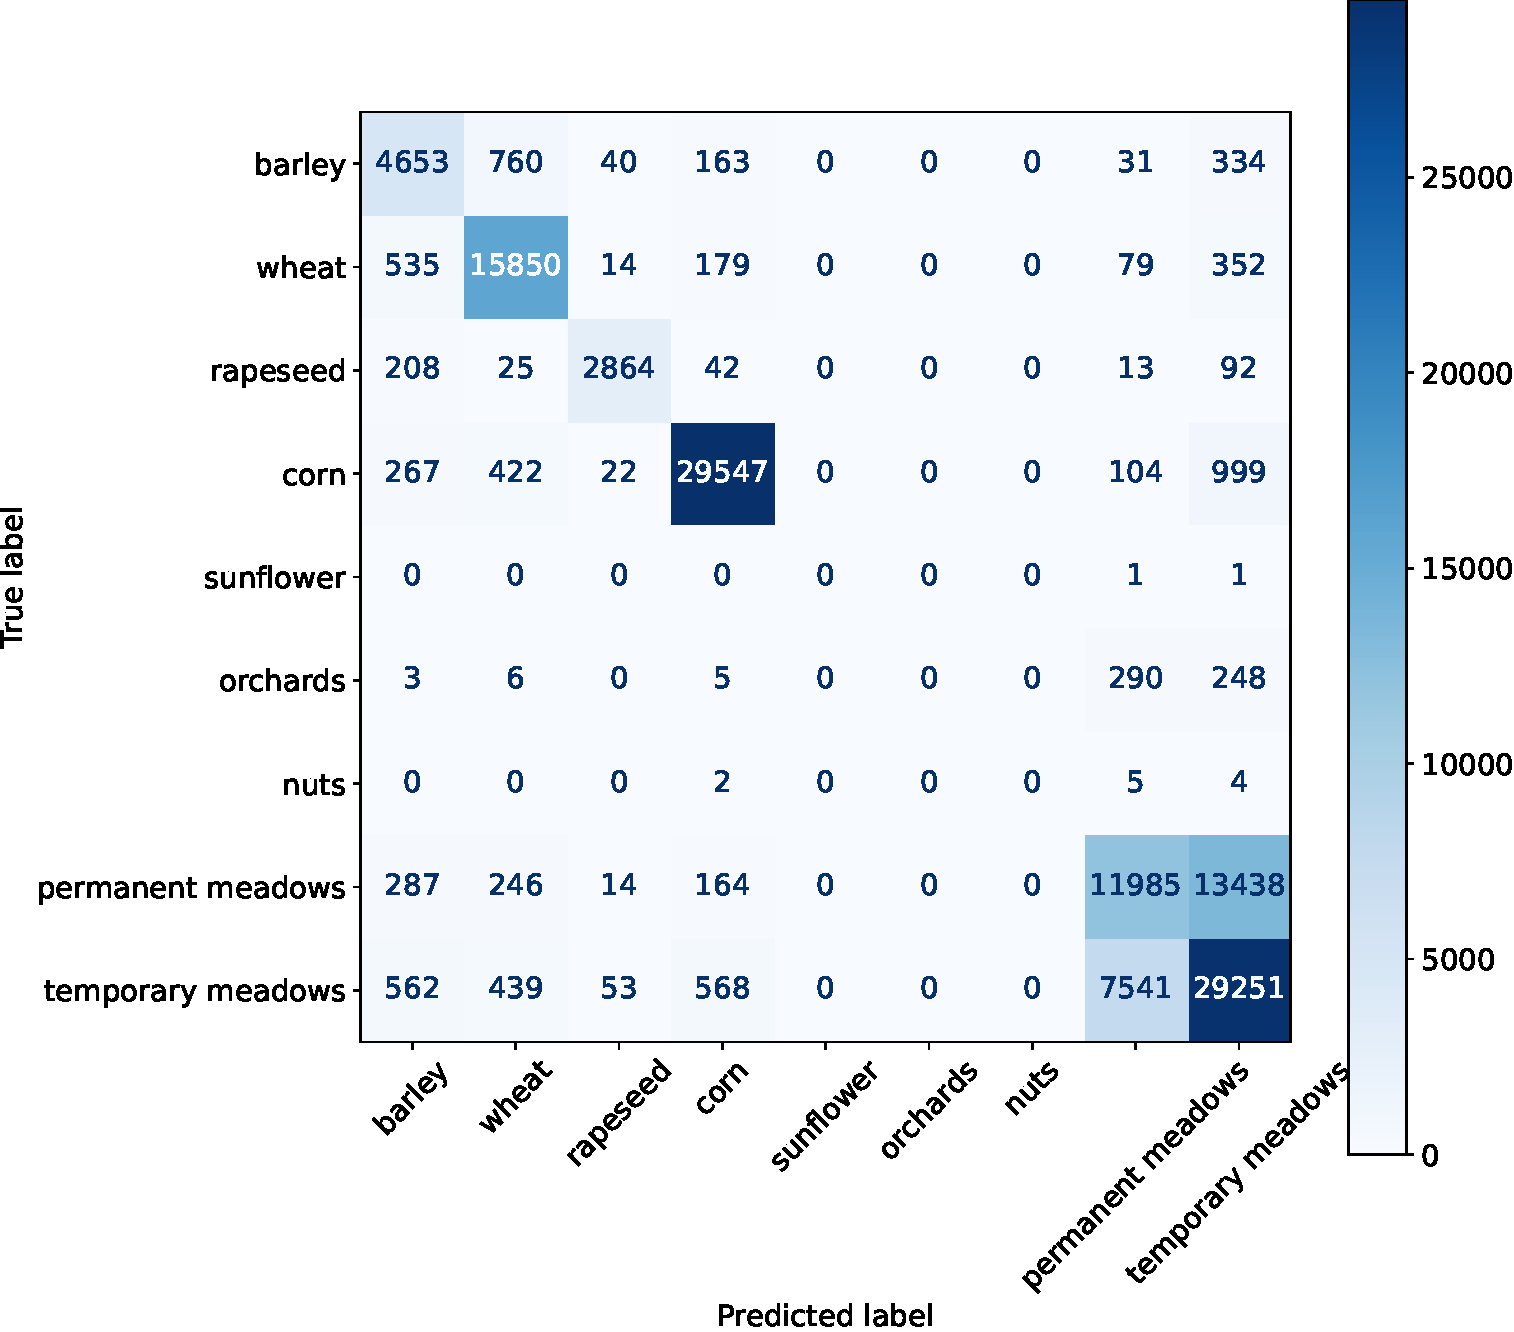
\includegraphics[width=.57\textwidth]{figures/aes_1_layer_mse_results/confusion_matrix_test.pdf}
% 	\caption{Confusion matrix of the FCN prediction for the testing data.}
% 	\label{confusion_matrix}
% \end{figure}
%In the Table \ref{Quantitative_results} we can see the summary results,
Table \ref{Quantitative_results} presents a performance comparison of our method with \DIFaddbegin \DIFadd{much deeper models, such as }\DIFaddend convolutional, recurrence and attention-based methods. 
TempCNN, OmniscCNN, LSTM, StarRNN, Transformer \DIFdelbegin \DIFdel{, }\DIFdelend \DIFaddbegin \DIFadd{presented in \mbox{%DIFAUXCMD
\cite{Russwurm2020} }\hskip0pt%DIFAUXCMD
}\DIFaddend and our proposed method \DIFdelbegin \DIFdel{with the generated representations as input to a FCN }\DIFdelend are evaluated by OA, average precision (AP), F1 score, and $\kappa$. 
Additionally, \DIFdelbegin \DIFdel{details on the processor used, }\DIFdelend the number of parameters \DIFdelbegin \DIFdel{, and runtime }\DIFdelend \DIFaddbegin \DIFadd{and runtime in iteratios per second }\DIFaddend ($it/s$) are presented. 
We present the results reported in \cite{Russwurm2020}\DIFdelbegin \DIFdel{, since the code used for those experiments is not publicly available and it is not straightforwardly reproducible}\DIFdelend . 
Notwithstanding, the same test data points were used in our experiments, hence, results are directly comparable.

\begin{table}[H]
	\centering
	\caption{Classification performance evaluation of benchmarked models by overall accuracy (OA), average precision (AP), F1 score (F1) and Cohen’s kappa coefficient ($\kappa$). All models were evaluated over the same testing dataset \DIFaddbeginFL \DIFaddFL{and on a processor Intel® Core™ i5-7200U CPU @ 2.5GHz, 4 cores, Dell Inc. Inspiron 15-3567 Intel® HD Graphics 620 (KBL GT2). In bold the best results are highlighted}\DIFaddendFL .}
	\footnotesize
	\begin{tabular}{c| c c c c c c}
	\hline
	    & TempCNN & OmniscCNN & LSTM            & \DIFdelbeginFL \DIFdelFL{StartRNN }\DIFdelendFL \DIFaddbeginFL \DIFaddFL{StarRNN }\DIFaddendFL & Transformer     & \textbf{AE-FCN}\\[1.1ex]
	\hline   
	OA  & 0.79    & 0.73      & \textbf{0.80}   & 0.79     & \textbf{0.80}  & \DIFdelbeginFL \textbf{\DIFdelFL{0.77}} %DIFAUXCMD
\DIFdelendFL \DIFaddbeginFL \DIFaddFL{0.77 }\DIFaddendFL \\
	AP  & 0.55    & 0.52      & 0.57            & 0.56     & 0.58           &  0.54\\
	F1  & 0.79    & 0.72      & 0.80            & 0.79     & 0.80           &  0.76\\
$\kappa$& 0.73    & 0.65      & 0.74            & 0.73     & 0.75           &  0.70\\ [1.2ex]
	\hline
\DIFdelbeginFL \DIFdelFL{Processor }%DIFDELCMD < &\multicolumn{5}{c}{\makecell{8X NVIDI Tesla P100 \\ 16GB/GPU 28,672 Total\\ NVIDIA CUDA Cores}} & \makecell{Intel® Core™ \\i5-1035G1 \\CPU @ 1.00GHz\\ $\times$8 Mesa Intel® \\UHD Graphics\\(ICL GT1)}\\ [%%%
\DIFdelFL{1.1ex}%DIFDELCMD < ] \hline
%DIFDELCMD < 	%%%
\DIFdelendFL N° param & 3,199,501 & 2,739,737 & 1,339,431     & 72,103   & 188,429       & \textbf{6,825} \\
\DIFdelbeginFL %DIFDELCMD < \makecell{Runtime in\\ $[it/s]$}  %%%
\DIFdelendFL \DIFaddbeginFL \makecell{Runtime in\\$[it/s]$}  \DIFaddendFL & \DIFdelbeginFL \DIFdelFL{1.25 }\DIFdelendFL \DIFaddbeginFL \DIFaddFL{0.70 }\DIFaddendFL & \DIFdelbeginFL \DIFdelFL{1.02      }\DIFdelendFL \DIFaddbeginFL \DIFaddFL{0.07 }\DIFaddendFL & \DIFdelbeginFL \DIFdelFL{1.16           }\DIFdelendFL \DIFaddbeginFL \DIFaddFL{0.12  }\DIFaddendFL & \DIFdelbeginFL \DIFdelFL{1.02     }\DIFdelendFL \DIFaddbeginFL \DIFaddFL{0.22 }\DIFaddendFL & \DIFdelbeginFL \DIFdelFL{1.20              }\DIFdelendFL \DIFaddbeginFL \DIFaddFL{0.44        }\DIFaddendFL & \DIFdelbeginFL \DIFdelFL{0.75 }\DIFdelendFL \DIFaddbeginFL \textbf{\DIFaddFL{23.8}} \DIFaddendFL \\
	\hline
\end{tabular}
\label{Quantitative_results}
\end{table}

% The OA achieved with our method is 0.74, while a Transformer model reaches 0.80. However, Transfomer is composed by 188,429 trainable parameters, while ours only needs 6,825, i.e., ~28 times less trainable parametes, which is directly related to the computational load and processing time. 
% Moreover, other complex convolutional models, such as TempCNN and OmniscCNN, achieve 0.79 and 0.73 OA, i.e., only 0.05 higher and 0.01 lower than our method respectively, but more 400 times more parameters.
% Likewise, Transformer's AA has the highest score 0.58, while our method reached 0.53, slightly below transformers but still within a competitive range.

% The F1 score, which balances precision and recall, and therefore provides a balanced assessment of the model, was also the highest in the LSTM and Transformer models with 0.80, while our representations-based FCN achieved 0.74, reflecting its ability to maintain a reasonable balance despite the imbalanced class distribution.
% Similarly, LSTM and Transformer models reach the highest Kappa's coefficient (0.75), while our method's is strongly penalized due mostly to the proportion of mismatches on barley, and permanent and temporary meadows. Although our method reaches 0.10 lower score than the competing models, it is still relatively good, especially considering the shallowness of the model.

Our representations-based approach combined with the FCN is substantially less computationally expensive than the other benchmarked methods, requiring only 6,825 trainable parameters, compared to the 1,338,431 for LSTM and 188,429 for Transformer. This means \DIFaddbegin \DIFadd{that }\DIFaddend our method uses roughly 200 and 28 times fewer parameters, respectively, compared to the two deep learning methods. This reduction directly impacts computational load and consequently processing time, as seen in the runtime of \DIFdelbegin \DIFdel{0.75 }\DIFdelend \DIFaddbegin \DIFadd{23.8 }\DIFaddend it/s \DIFdelbegin \DIFdel{for FCN, which , despite running on much lower capacity hardware, is just slightly slower than Transformer (1.20 it/s) and other sophisticated models such as TempCNN (1.25 }\DIFdelend \DIFaddbegin \DIFadd{obtained with our method, which is more than 30 times higher than the best of these deep models in terms of runtime, TempCNN (0.70 }\DIFaddend it/s) and \DIFdelbegin \DIFdel{OmniscCNN (1.02 }\DIFdelend \DIFaddbegin \DIFadd{more than 50 times higher than Transformer (0.44 }\DIFaddend it/s).

In addition to this substantial reduction of trainable parameters, our method maintains competitive classification accuracy, achieving an OA of \DIFdelbegin \DIFdel{0.767}\DIFdelend \DIFaddbegin \DIFadd{0.7706}\DIFaddend , just $3\%$ lower than Transformer's OA of 0.80. Furthermore, the accuracy of our method is comparable to TempCNN (OA=0.79) and \DIFaddbegin \DIFadd{4\% better than }\DIFaddend OmniscCNN (OA=0.73). However, these two approaches are computationally far more expensive, requiring approximately 400 times more parameters than AE-derived representations within a simple FCN (AE-FCN).

In terms of metrics that weight class imbalance, \DIFdelbegin \DIFdel{Transformer has the highest AP of 0.58, while AE-FCN obtains a competitive 0.54. }\DIFdelend LSTM and Transformer obtained the highest F1 score (both 0.80), whereas AE-FCN achieves a competitive 0.76, indicating a balanced performance despite having far fewer parameters. Similarly, LSTM and Transformer have the highest $\kappa$ score (0.75), with AE-FCN scoring 0.70, which is penalized owing to mismatches in particular classes but remains effective given the model's simplicity.

\subsection{Qualitative results}

%\textcolor{yellow}{\textbf{This part belong to the section methodology (CHECK!)}}
%In this section we use 
%DIF < Google Earth Engine (GEE) was used for download a multitemporal multispectral image of Sentinel 2 sensor in the FRH04 region of the 2017 year (see Figure \ref{fig:gee_img}) in order to obtain classification maps. \\
%DIF > Google Earth Engine (GEE) was used for download a multitemporal multispectral image of Sentinel-2 sensor in the FRH04 region of the 2017 year (see Figure \ref{fig:gee_img}) in order to obtain classification maps. \\
% As BreizhCrops data are sparse geographic points and not images, a qualitative assessment based on classification maps cannot be directly performed on this dataset. 
% Nevertheless, 
To enable a qualitative analysis over a contiguous spatial extent and not simply on a tabulated dataset, 67 Sentinel-2 multispectral images from 2017 of a subregion in FRH04 (test region) were downloaded and preprocessed.
A representative area was defined drawing a polygon where most of the classes (barley, wheat, corn, rapeseed, temporary meadows and permanent meadows) are present (Figure \ref{fig:gee_img_a}). 
% As for the BreizCrops dataset, only 10m and 20m resolution bands (resampled to 10m) were used. 
% Besides, temporal embeddings described in subsection \ref{data_preprocessing}, as well as spectral indices mentioned in subsection \ref{dataset} are added as features.
% \begin{figure}[H]
% 	\centering
% 	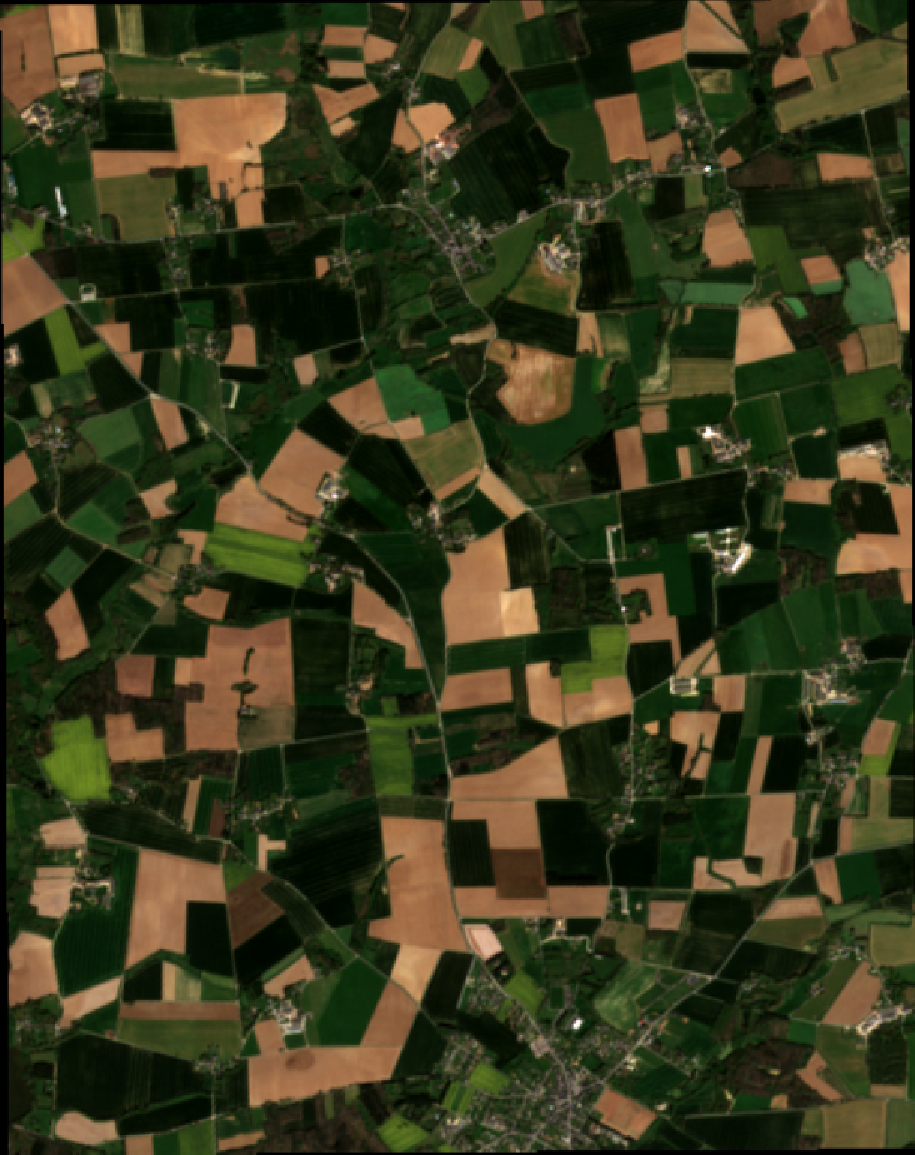
\includegraphics[height=0.33\linewidth,width=0.3\linewidth]{figures/reconstruction_errors/test_aoi_RGB.pdf}
% 	\caption{True color image of the study area in 2017.}
% 	\label{fig:gee_img}
% \end{figure}

%The first step was to draw a polygon in this region where there are the majority of the classes, after this we download all images considering only 10 bands (10 and 20 meters of resolution). The second step was to do a preprocessing where was necessary to add the spectral indices and the day of the year in each image. After this we obtained the representations of this multitemporal multispectral image using the AEs trained previously. In the Figure \ref{representations} we can see the feature second of the representations of each AE.
Representations for this study area are produced by passing individual pixels from the imagery dataset through the inference workflow outlined in Figure \ref{Inference}. \DIFdelbegin \DIFdel{Exemplary composite }\DIFdelend \DIFaddbegin \DIFadd{Composite }\DIFaddend images generated by combining three random representations are presented in Figures \ref{fig:color_map_b}, \ref{fig:color_map_c}, \ref{fig:color_map_d}, \ref{fig:color_map_e}, \ref{fig:color_map_f}, \ref{fig:color_map_g} and \ref{fig:color_map_h}, which clearly contrast the crop fields in the new representation space.
% The false color images generated by combining three random representations bands presented in Figures \ref{fig:color_map_a}, \ref{fig:color_map_b} and \ref{fig:color_map_c}, as well as individual representations shown in Figure \ref{representations}, contrast the crop fields in the new representations space.
\begin{figure}[H]
	\centering
	\begin{subfigure}[t]{0.23\linewidth}
		\centering
	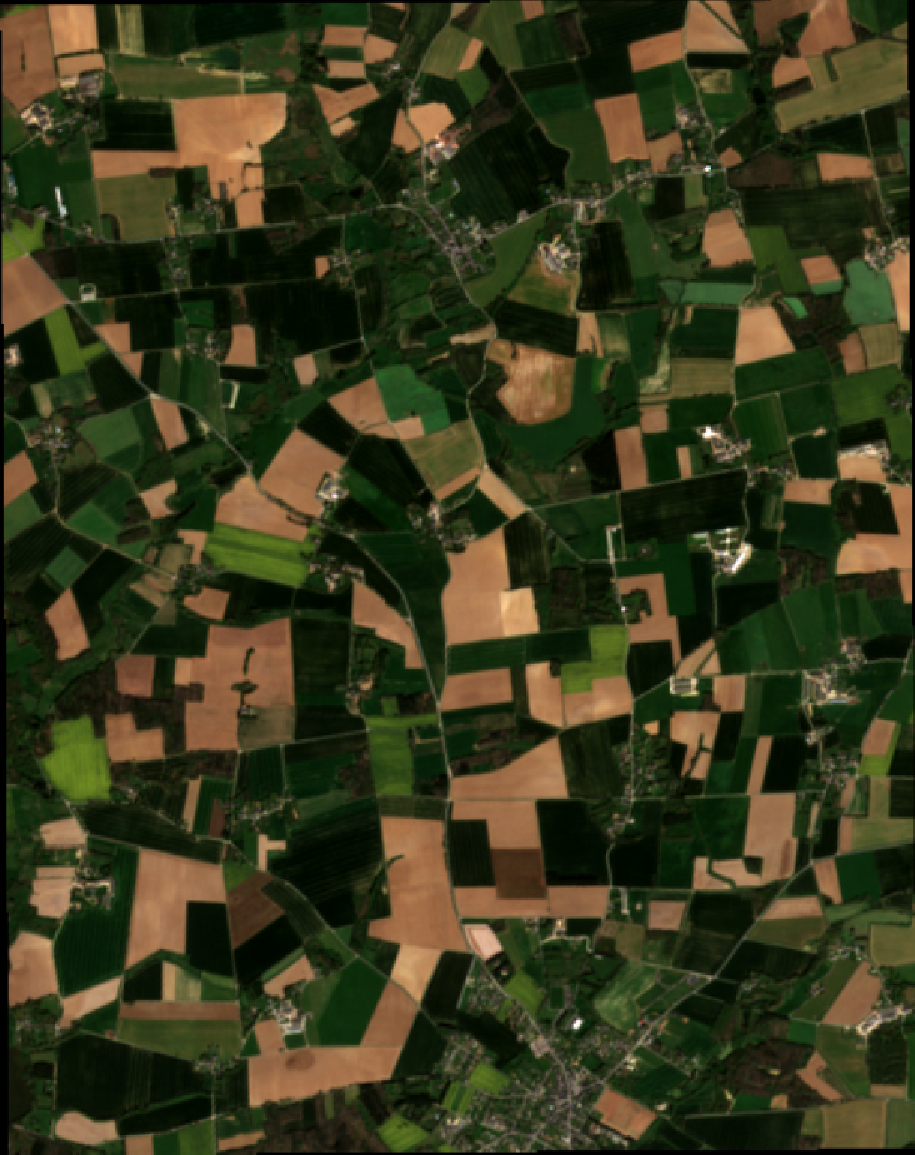
\includegraphics[width=0.95\linewidth]{figures/reconstruction_errors/test_aoi_RGB.pdf}
	\caption{}
	\label{fig:gee_img_a}
	\end{subfigure}
	\begin{subfigure}[t]{0.23\linewidth}
		\centering
    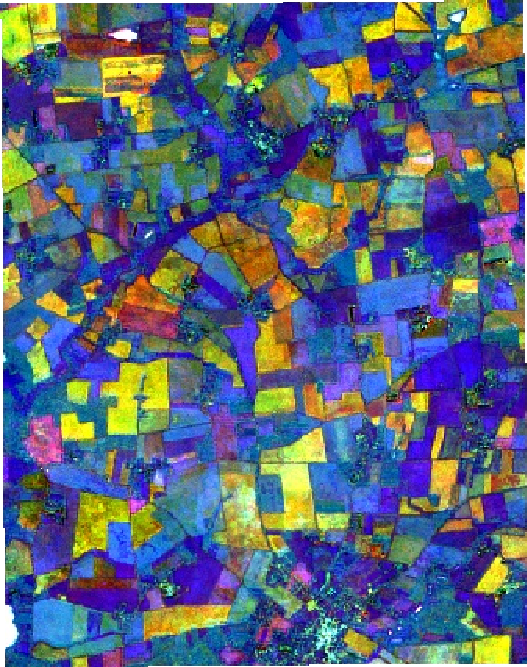
\includegraphics[width=0.95\linewidth]{figures/aes_1_layer_mse_results/composites/composite_image_1.pdf}
	\caption{}
	\label{fig:color_map_b}
	\end{subfigure}
	\begin{subfigure}[t]{0.23\linewidth}
		\centering
	  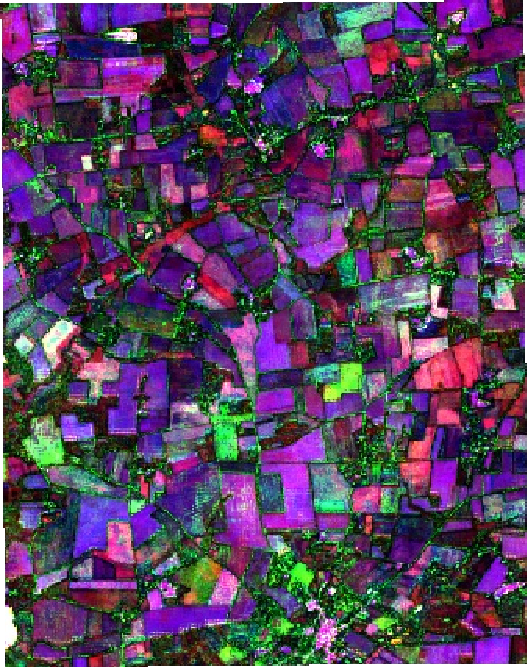
\includegraphics[width=0.95\linewidth]{figures/aes_1_layer_mse_results/composites/composite_image_598481.pdf}
	\caption{}
	\label{fig:color_map_c}
	\end{subfigure}
	\begin{subfigure}[t]{0.23\linewidth}
		\centering
	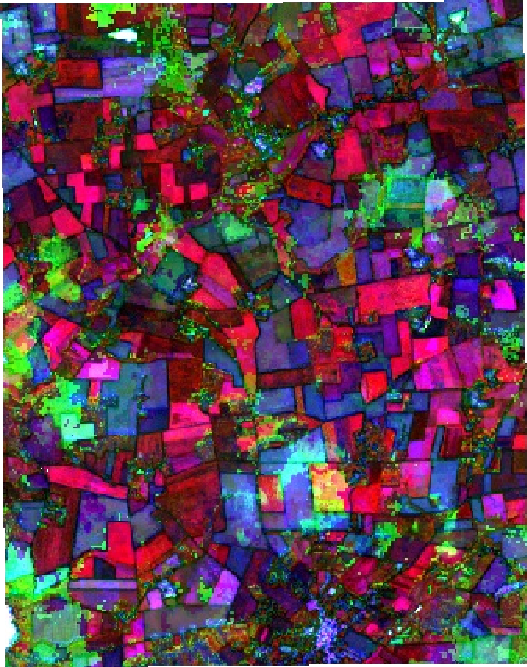
\includegraphics[width=0.95\linewidth]{figures/aes_1_layer_mse_results/composites/composite_image_3011141.pdf}
    \caption{}
	\label{fig:color_map_d}
	\end{subfigure}\\[0.2cm]
    \begin{subfigure}[t]{0.23\linewidth}
		\centering
	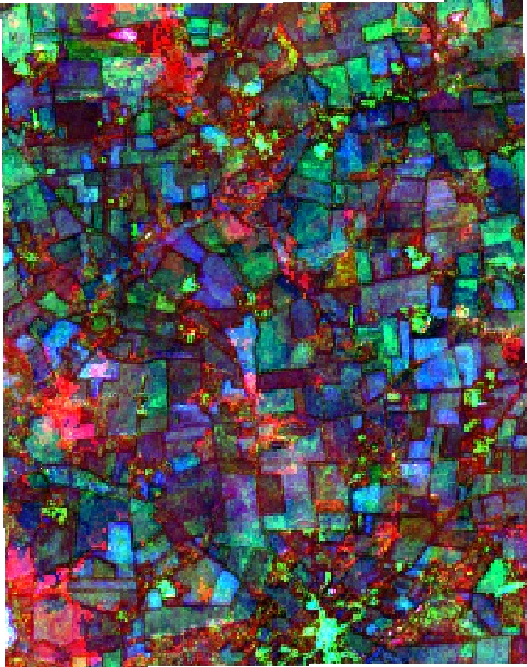
\includegraphics[width=0.95\linewidth]{figures/aes_1_layer_mse_results/composites/composite_image_456657.pdf}
    \caption{}
	\label{fig:color_map_e}
	\end{subfigure}
    \begin{subfigure}[t]{0.23\linewidth}
		\centering
	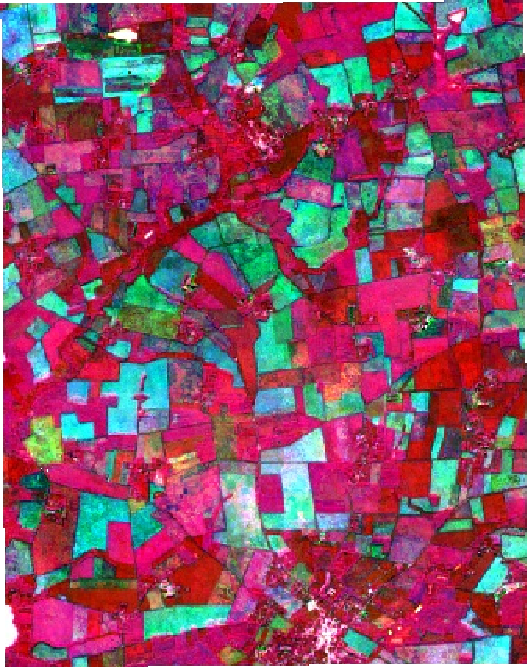
\includegraphics[width=0.95\linewidth]{figures/aes_1_layer_mse_results/composites/composite_image_201032.pdf}
    \caption{}
	\label{fig:color_map_f}
	\end{subfigure}
    \begin{subfigure}[t]{0.23\linewidth}
		\centering
	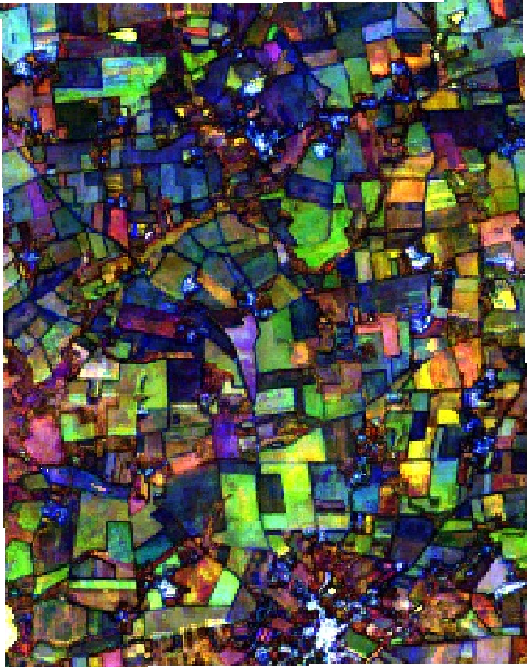
\includegraphics[width=0.95\linewidth]{figures/aes_1_layer_mse_results/composites/composite_image_514283.pdf}
    \caption{}
	\label{fig:color_map_g}
	\end{subfigure}
    \begin{subfigure}[t]{0.23\linewidth}
		\centering
	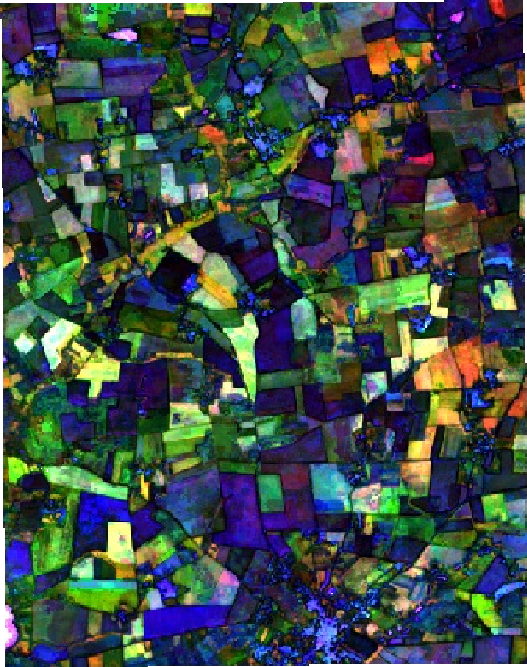
\includegraphics[width=0.95\linewidth]{figures/aes_1_layer_mse_results/composites/composite_image_2479133.pdf}
    \caption{}
	\label{fig:color_map_h}
	\end{subfigure}
	\caption{(a) True color image of the study area in 2017 and composites images generated by combining three random representations per map (b) 9-64-30, (c) 59-84-81, (d) 30-11-141, (e) 45-66-57, (f) 20-10-32, (g) 5-142-83 and (h) 24-79-133.}
	\label{color_maps}
\end{figure}

% \begin{figure}[H]
% 	\centering
% 	\begin{subfigure}[t]{0.23\linewidth}
% 		\centering
% 		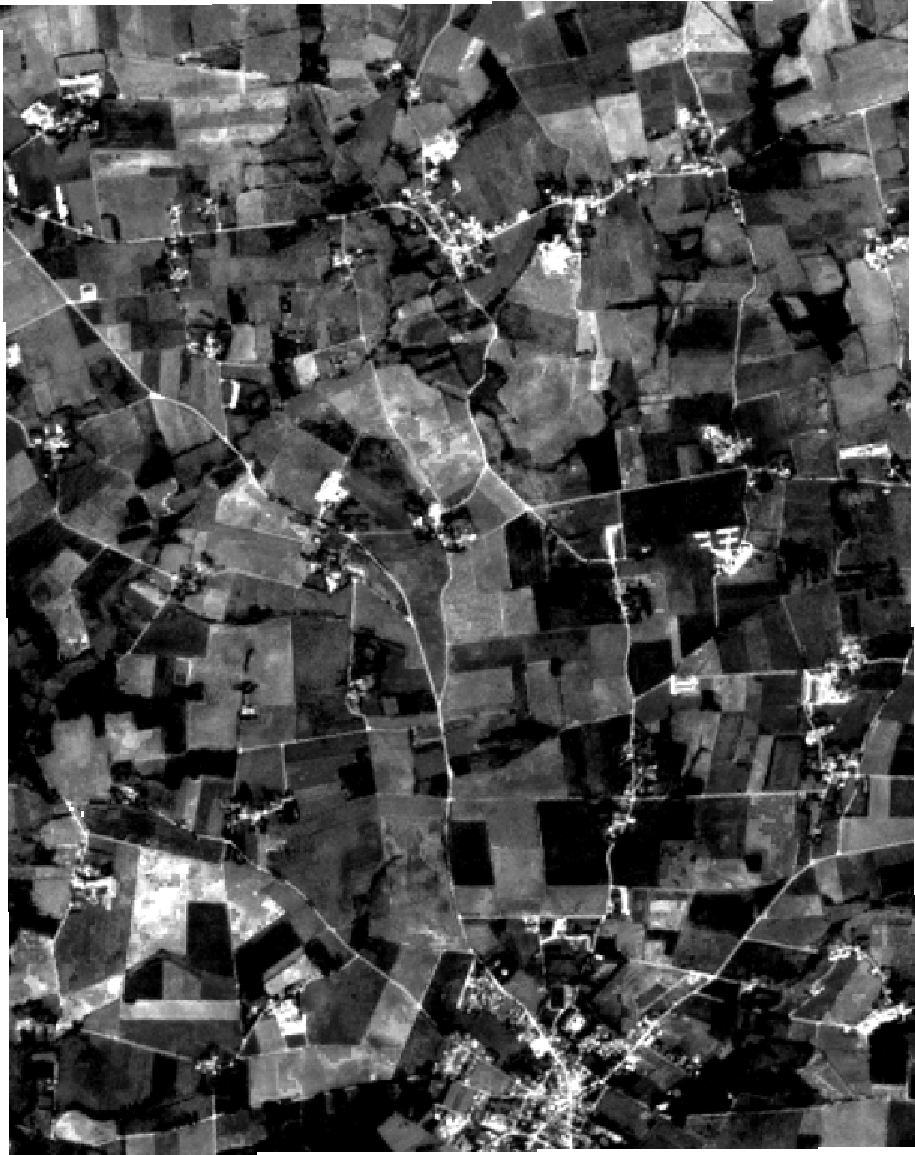
\includegraphics[height=\linewidth,width=0.95\linewidth]{figures/reconstruction_errors/reconstruction_B2_AEs0.pdf}
% 	\caption{}
% 	\label{fig:r_aes_b2_0}
% 	\end{subfigure}
% 	\begin{subfigure}[t]{0.23\linewidth}
% 		\centering
% 	  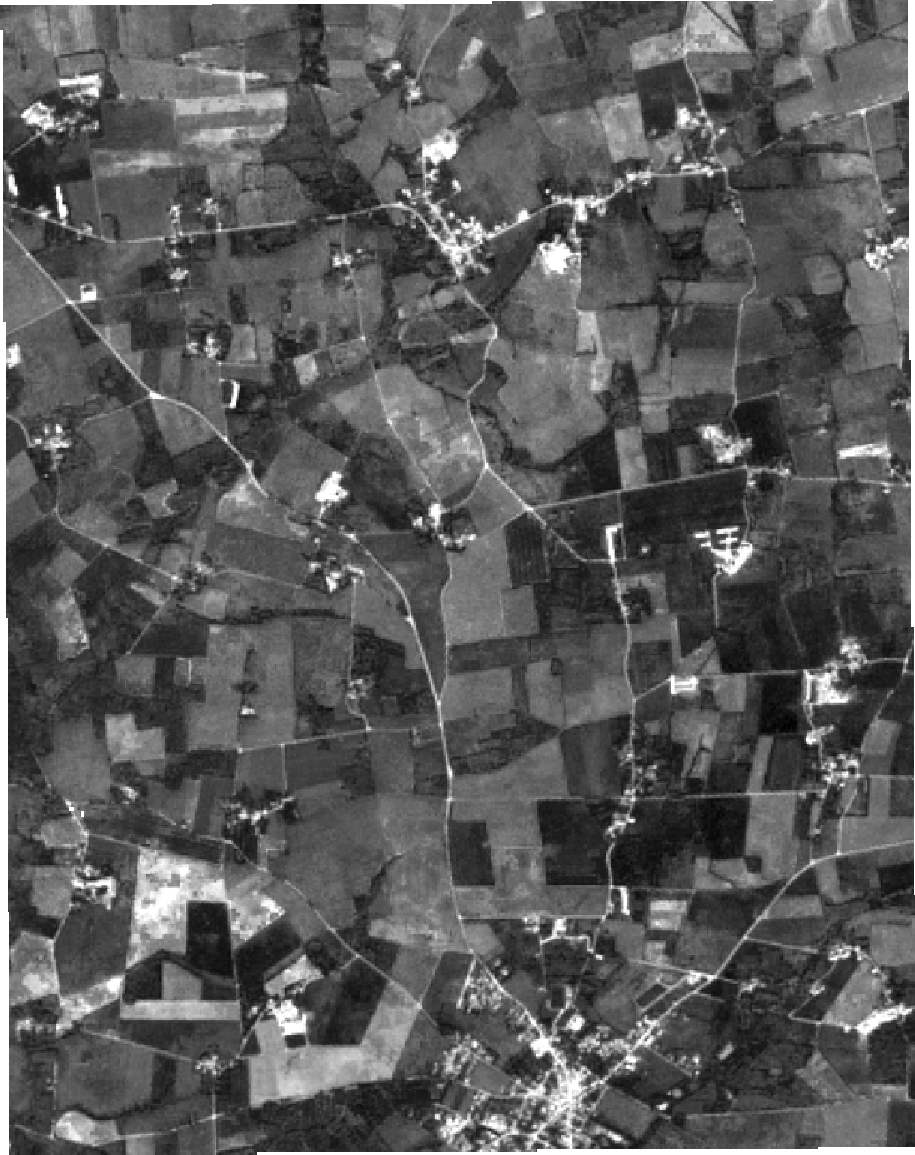
\includegraphics[height=\linewidth,width=0.95\linewidth]{figures/reconstruction_errors/reconstruction_B2_AEs1.pdf}
% 	\caption{}
% 	\label{fig:r_aes_b2_1}
% 	\end{subfigure}
% 	\begin{subfigure}[t]{0.23\linewidth}
% 		\centering
% 		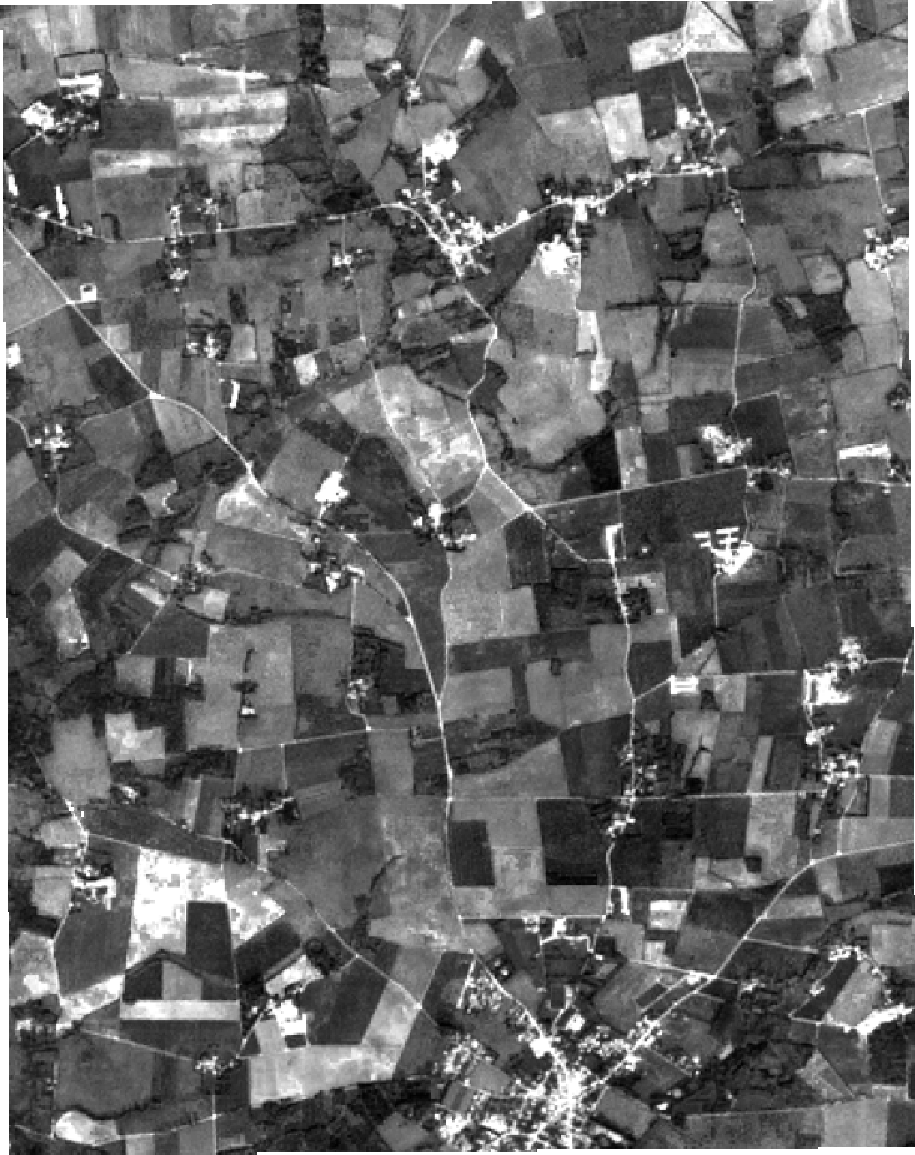
\includegraphics[height=\linewidth,width=0.95\linewidth]{figures/reconstruction_errors/reconstruction_B2_AEs2.pdf}
%     \caption{}
% 	\label{fig:r_aes_b2_2}
% 	\end{subfigure}
% 	\begin{subfigure}[t]{0.23\linewidth}
% 		\centering
% 		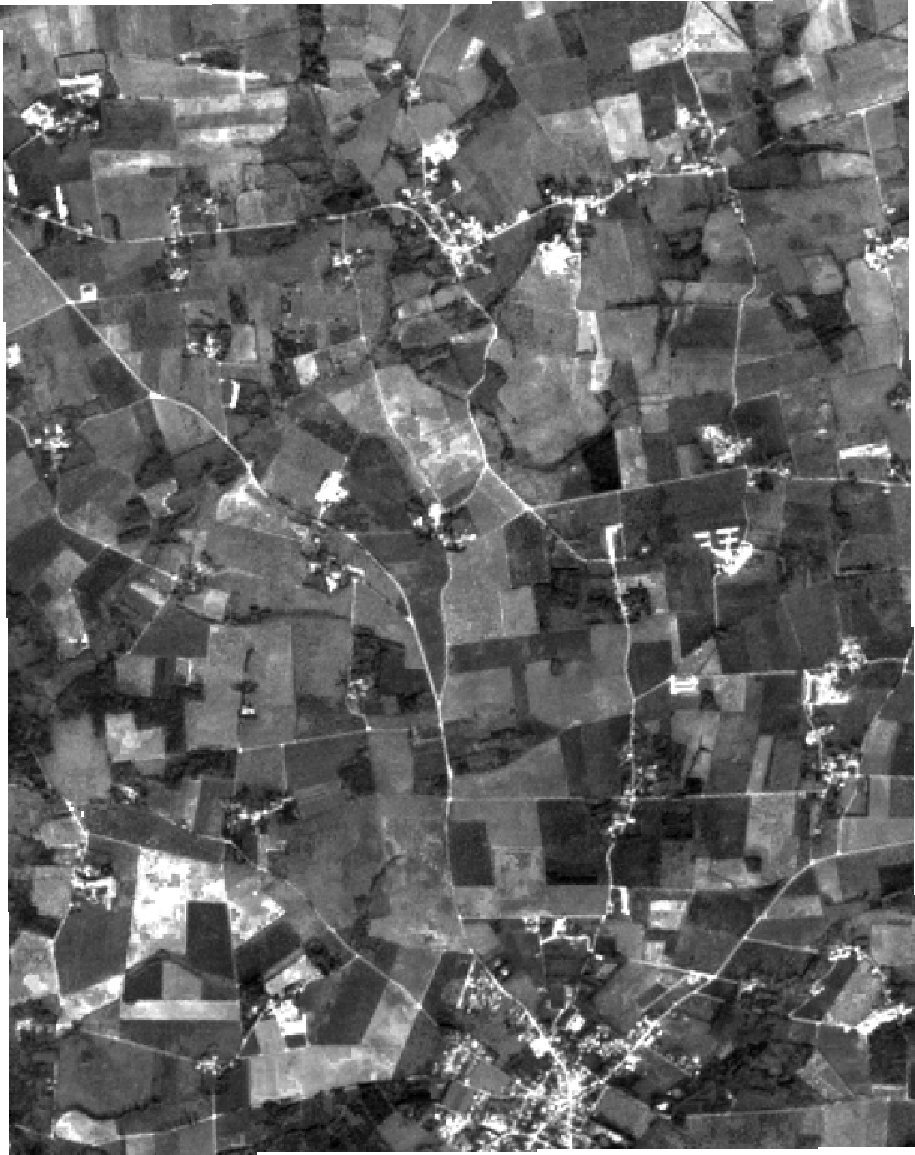
\includegraphics[height=\linewidth,width=0.95\linewidth]{figures/reconstruction_errors/reconstruction_B2_AEs3.pdf}
%     \caption{}
% 	\label{fig:r_aes_b2_3}
% 	\end{subfigure}\\[0.2cm]
% 	\begin{subfigure}[t]{0.23\linewidth}
% 		\centering
% 		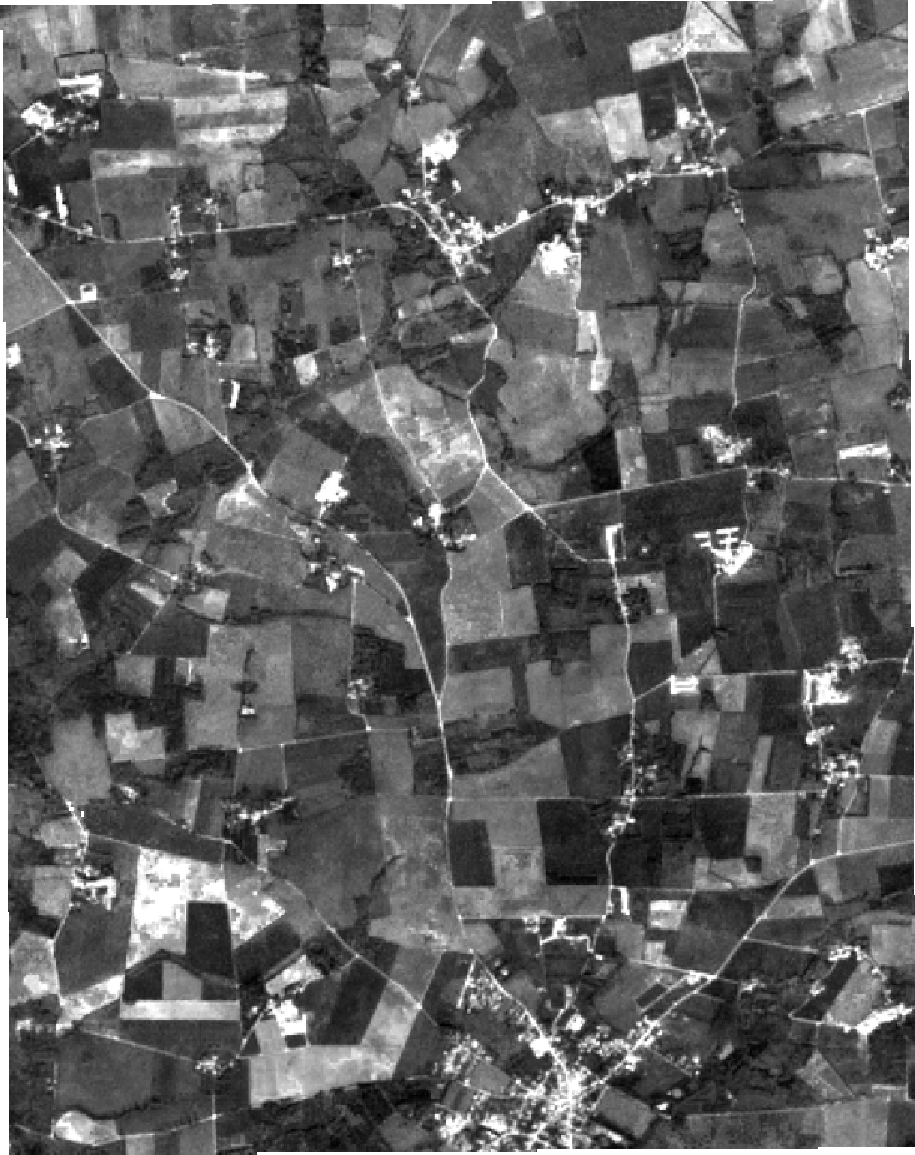
\includegraphics[height=\linewidth,width=0.95\linewidth]{figures/reconstruction_errors/reconstruction_B2_AEs4.pdf}
% 	 \caption{}
% 	\label{fig:r_aes_b2_4}
% 	\end{subfigure}
% 	\begin{subfigure}[t]{0.23\linewidth}
% 		\centering
% 		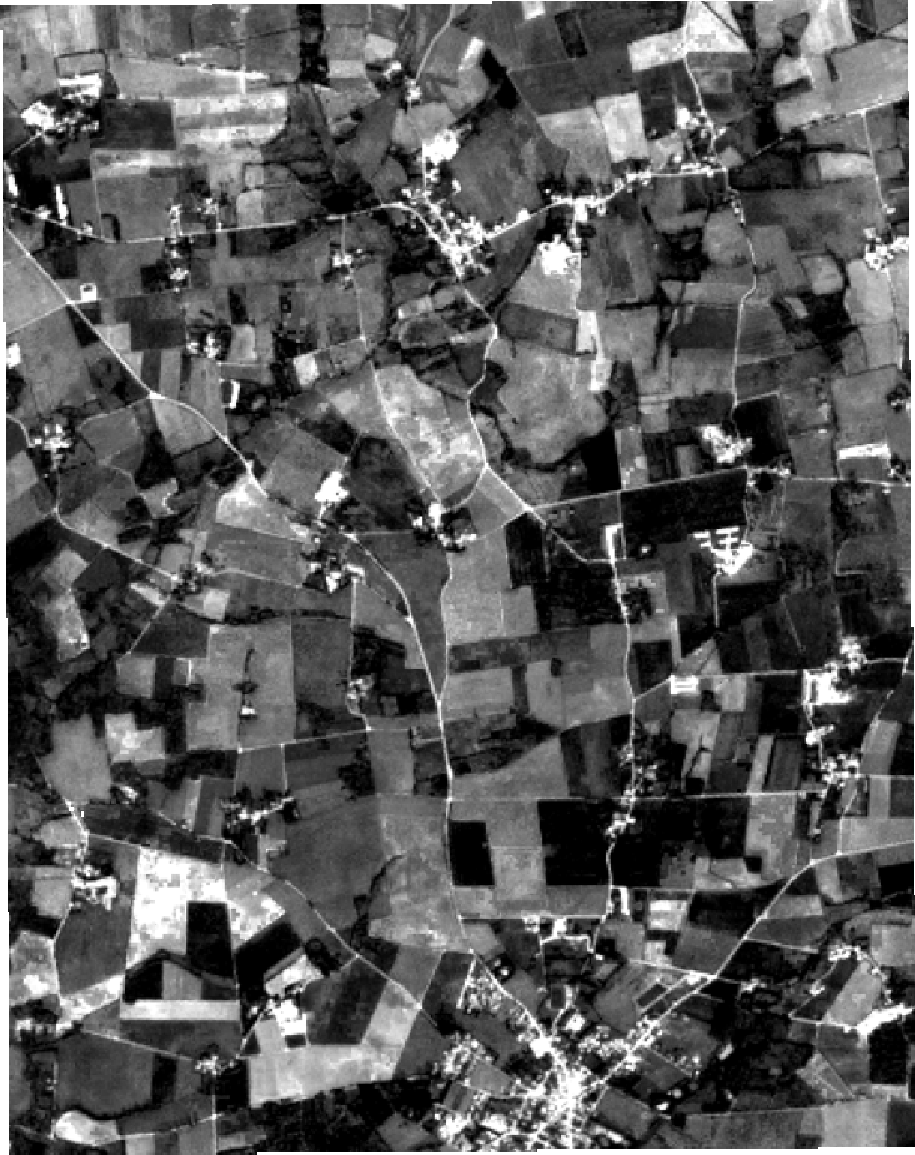
\includegraphics[height=\linewidth,width=0.95\linewidth]{figures/reconstruction_errors/reconstruction_B2_AEs5.pdf}
%     \caption{}
% 	\label{fig:r_aes_b2_5}
% 	\end{subfigure}
% 	\begin{subfigure}[t]{0.23\linewidth}
% 		\centering
% 		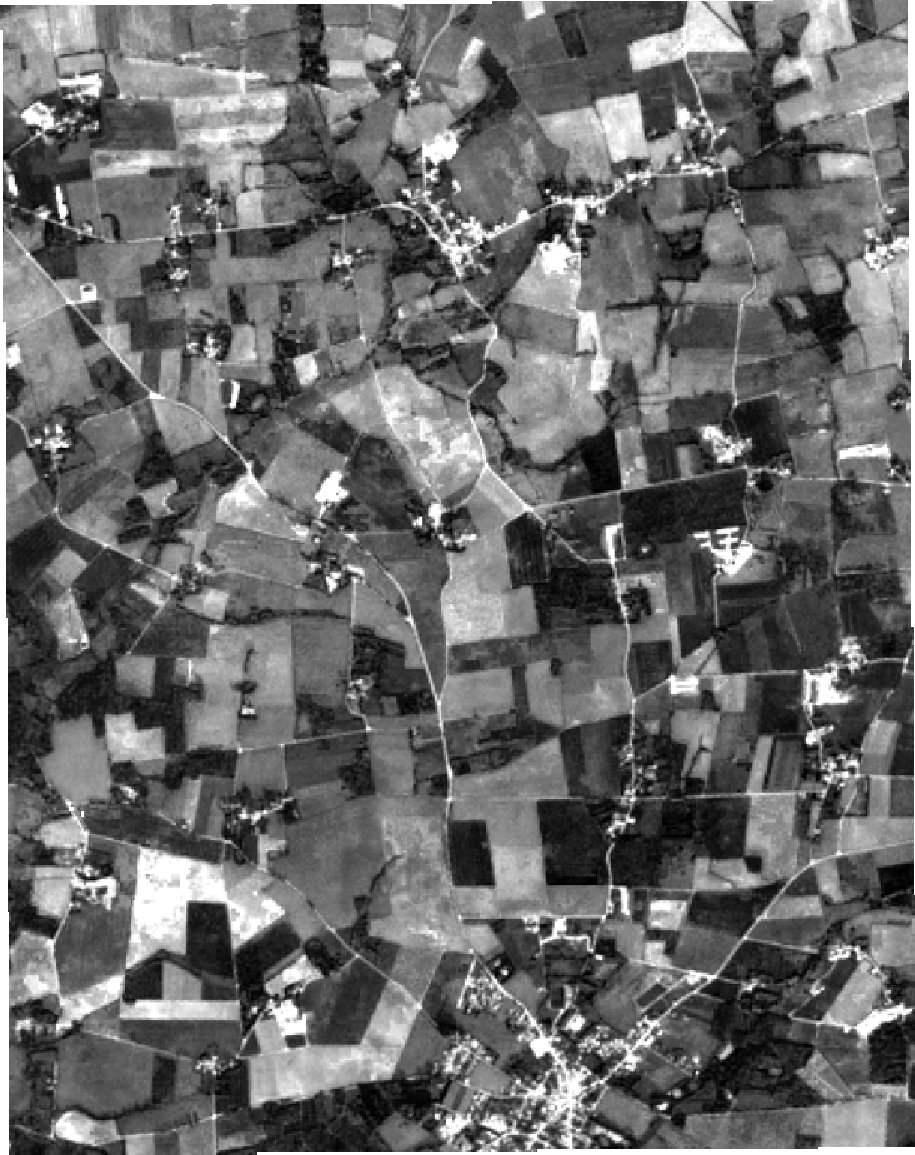
\includegraphics[height=\linewidth,width=0.95\linewidth]{figures/reconstruction_errors/reconstruction_B2_AEs6.pdf}
% 	\caption{}
% 	\label{fig:r_aes_b2_6}
% 	\end{subfigure}
% 	\begin{subfigure}[t]{0.23\linewidth}
% 		\centering
% 		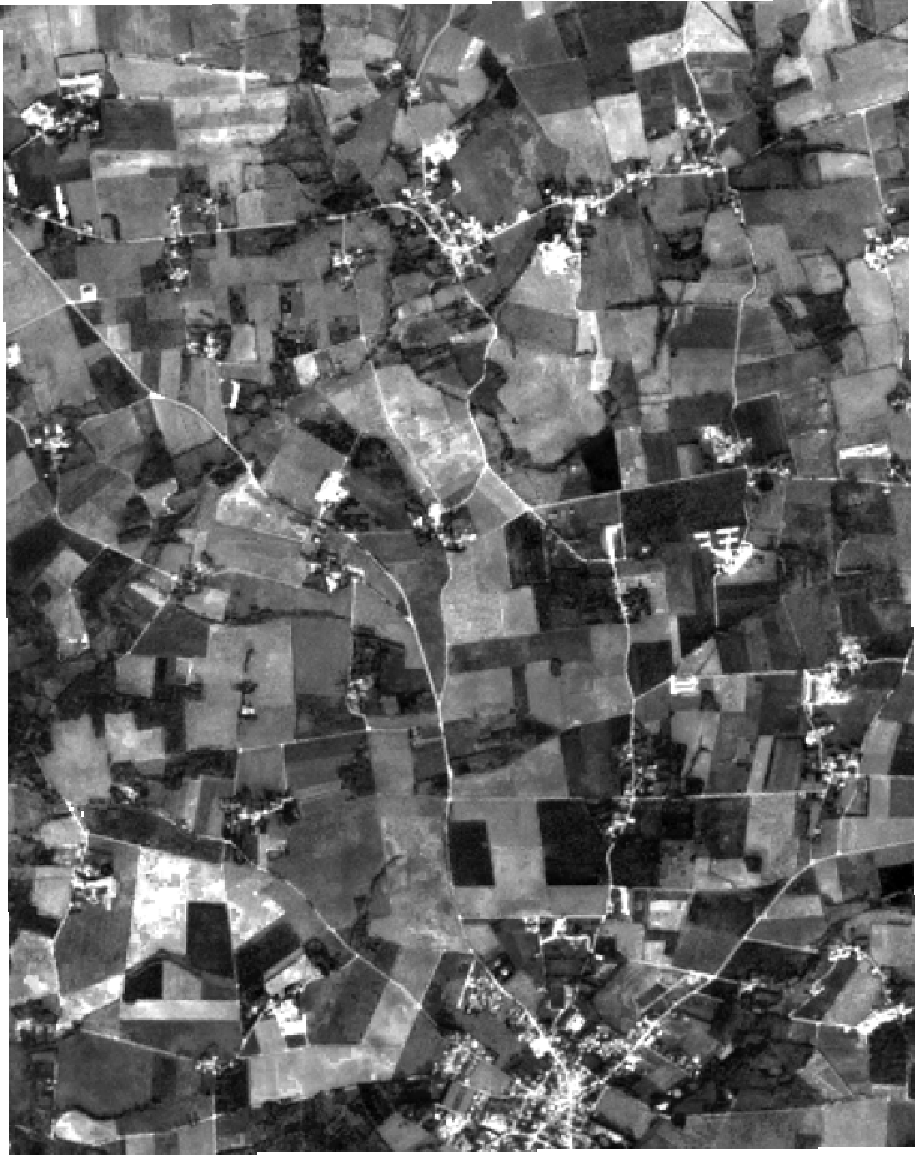
\includegraphics[height=\linewidth,width=0.95\linewidth]{figures/reconstruction_errors/reconstruction_B2_AEs7.pdf}
% 	\caption{}
% 	\label{fig:r_aes_b2_7}
% 	\end{subfigure}
% 	\caption{Visualization of a subset of the representation bands produced by our RL AE-based framework. We show here only 8 out of $9 \times 15$ available representations.}
% 	\label{representations}
% \end{figure}

% \begin{figure}[H]
% 	\centering
% 	\begin{subfigure}[t]{0.3\linewidth}
% 		\centering
% 		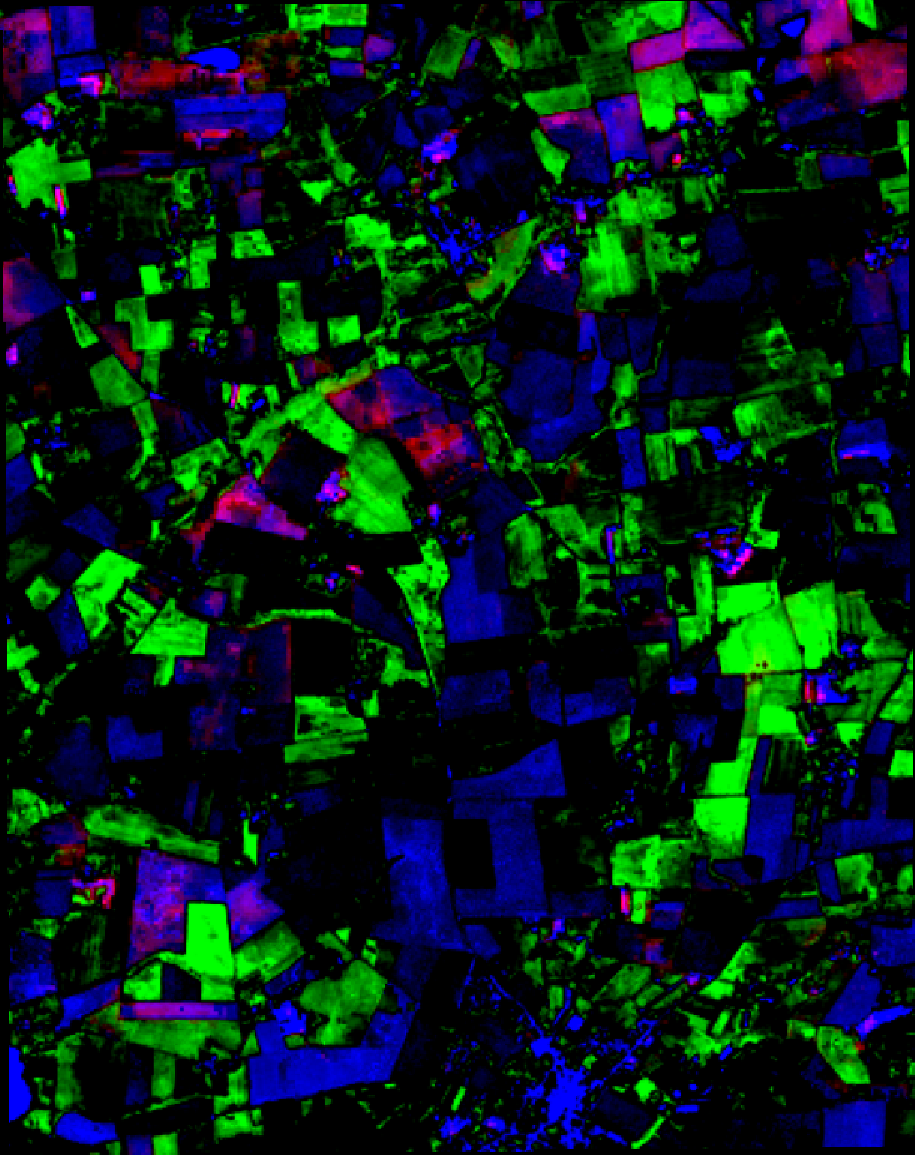
\includegraphics[width=0.8\linewidth]{figures/combinations/combinations_[59, 84, 81].pdf}
% 	\caption{}
% 	\label{fig:color_map_a}
% 	\end{subfigure}
% 	\begin{subfigure}[t]{0.3\linewidth}
% 		\centering
% 	  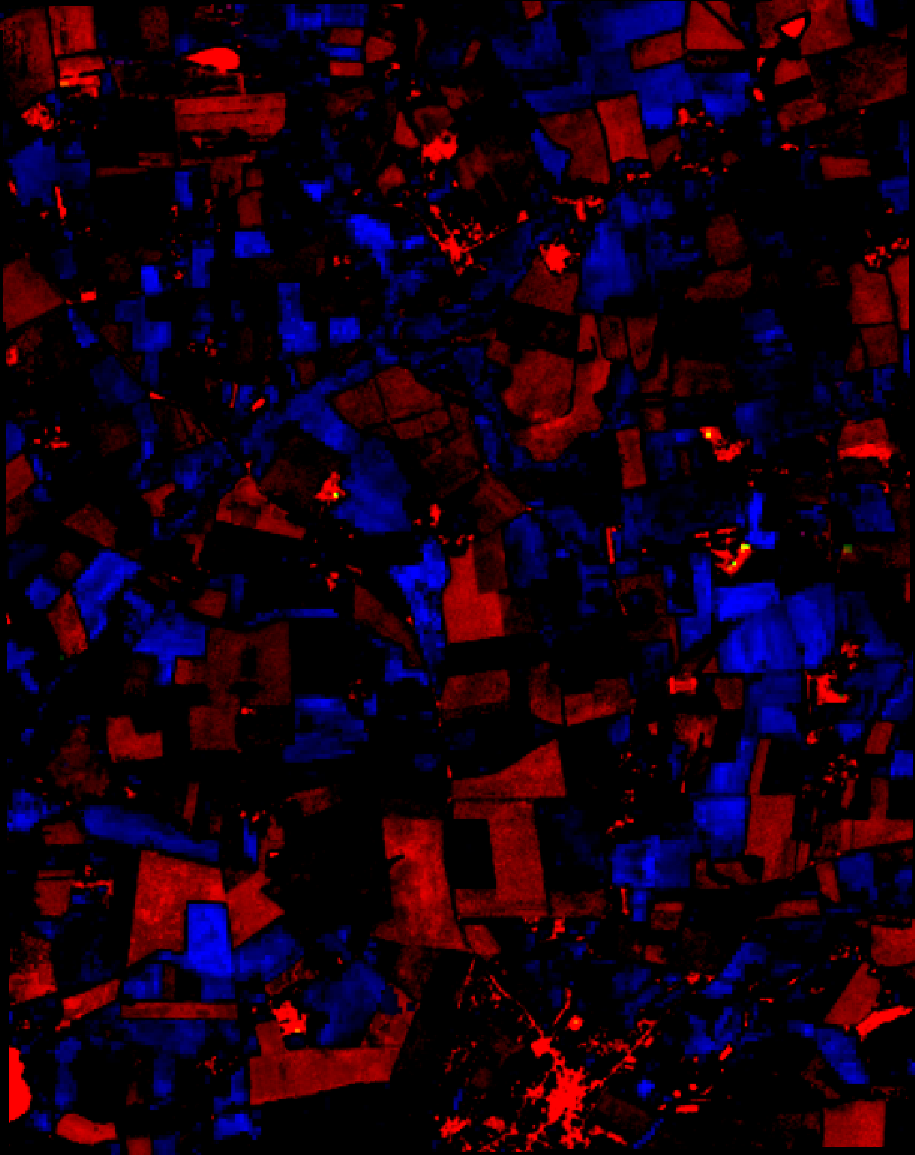
\includegraphics[width=0.8\linewidth]{figures/combinations/combinations_[30, 11, 141].pdf}
% 	\caption{}
% 	\label{fig:color_map_b}
% 	\end{subfigure}
% 	\begin{subfigure}[t]{0.3\linewidth}
% 		\centering
% 		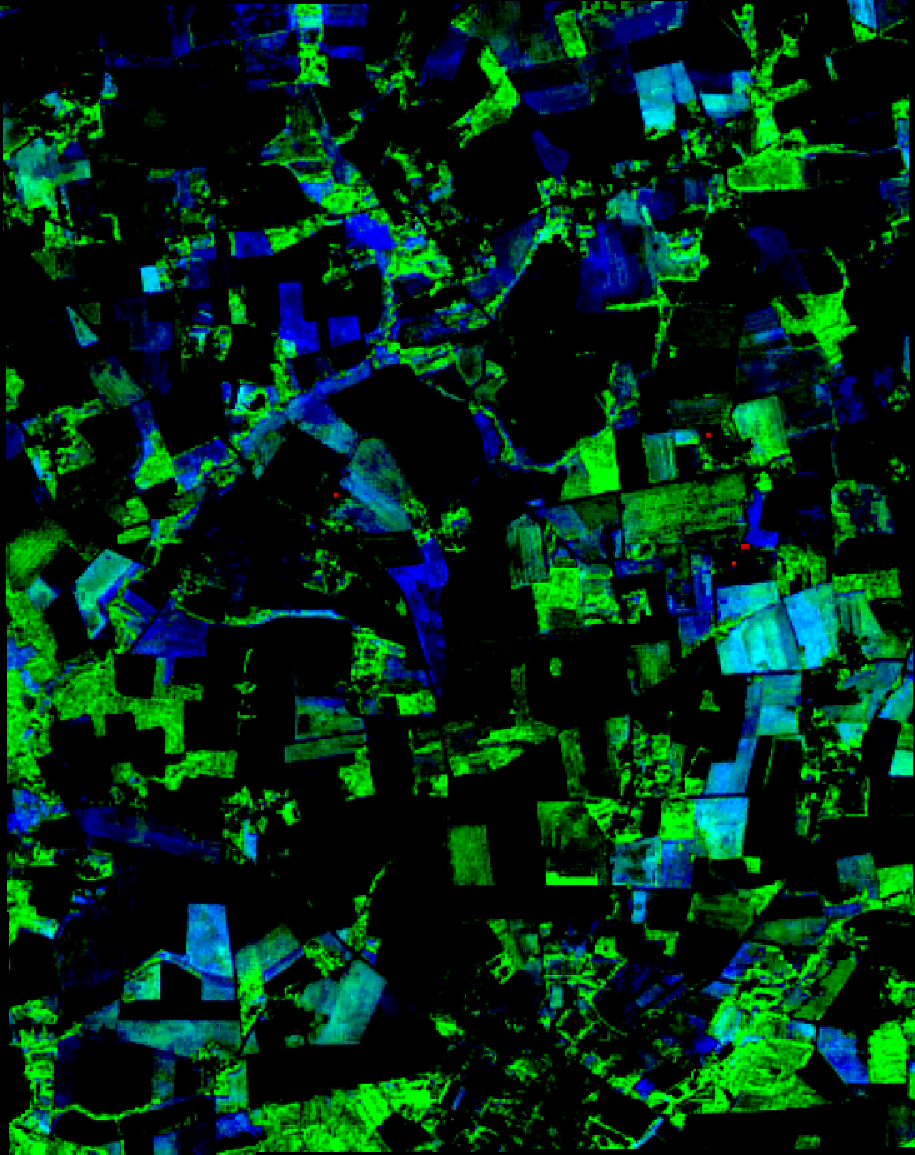
\includegraphics[width=0.8\linewidth]{figures/combinations/combinations_[45, 66, 57].pdf}
%     \caption{}
% 	\label{fig:color_map_c}
% 	\end{subfigure}
% 	\caption{Color maps of the representations with band combinations (a) 59,84,81, (b) 30,11,141 and (c) 45,66,57.}
% 	\label{color_maps}
% \end{figure}

% A classification map produced by the trained classification FCN, with the representations as input data, is presented in Figure \ref{fig:classification_pixel_level} together with the ground truth \ref{fig:frh04_labels}. In addition, a field-wise classification was performed by assigning to each field polygon the mode of the predicted class for pixels within the polygon. Field-based classification map is shown in Figure \ref{fig:classification_map_field}.\\

A classification map produced by our method is presented in Figure \ref{fig:maps}. 
Figure \DIFdelbegin \DIFdel{\ref{fig:classification_pixel_level} }\DIFdelend \DIFaddbegin \DIFadd{\ref{fig:test_aoi_pixel-wise} }\DIFaddend illustrates a pixel-based classification, i.e., without considering field boundaries or spatial context. Misclassifications are mainly seen  near field edges, since these are not pure pixels and often contain mixed spectral data. 

To better illustrate the potential of our method in real-world activities, Figure \DIFdelbegin \DIFdel{\ref{fig:classification_map_field} }\DIFdelend \DIFaddbegin \DIFadd{\ref{fig:test_aoi_field-base} }\DIFaddend presents a field-based classification map, where the output of our method is post-processed to group the pixel-wise predictions into polygon-level prediction by computing the mode of predictions within the field borders. This map preserves field structure, creating a more coherent and interpretable map. The strong similarity between Figures \DIFdelbegin \DIFdel{\ref{fig:frh04_labels} and \ref{fig:classification_map_field} }\DIFdelend \DIFaddbegin \DIFadd{\ref{fig:test_aoi_gt} and \ref{fig:test_aoi_field-base} }\DIFaddend show that the representations are sufficiently representative for crop type classification. 
\DIFaddbegin \DIFadd{Figure \ref{fig:true_positive_map} is a map showing correctly classified fields in green and misclassified fields in red.
}\DIFaddend 

% \begin{figure}[H]
% 	\centering
% 	\begin{subfigure}[t]{0.3\linewidth}
% 	\centering
% 	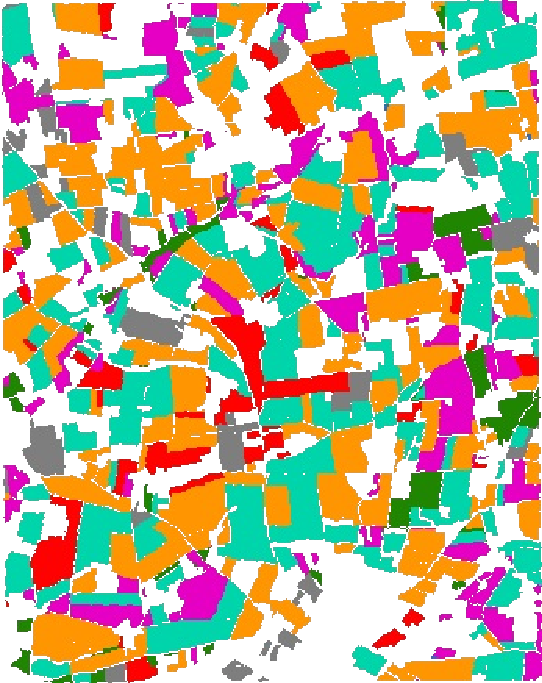
\includegraphics[height=\linewidth]{figures/aes_1_layer_mse_results/classification_maps/labels.pdf}
% 	\caption{}
% 	\label{fig:frh04_labels}
% 	\end{subfigure}\hspace{-1.5mm}
% 	\begin{subfigure}[t]{0.3\linewidth}
% 	  \includegraphics[height=\linewidth]{figures/aes_1_layer_mse_results/classification_maps/prediction_pixel_level.pdf}
% 	\caption{}
% 	\label{fig:classification_pixel_level}
% 	\end{subfigure}\hspace{-6.5mm} 
% 	\begin{subfigure}[t]{0.3\linewidth}
% 	\centering
%     \includegraphics[height=\linewidth]{figures/aes_1_layer_mse_results/classification_maps/prediction_polygon_base_with_labels.png}
% 	  \caption{}
% 	  \label{fig:classification_map_field}
% 	\end{subfigure}
% 	\caption{(a) Study area ground truth at field level (polygons), (b) representations-based fully connected network (FCN) pixel-wise classification (raster) and (c) representations-based FCN field-based classification (polygons).}
% 	\label{fig:maps}
% \end{figure}

\begin{figure}[H]
    % \hspace{-1.5mm}
	\DIFdelbeginFL %DIFDELCMD < \begin{subfigure}[t]{0.28\linewidth}
%DIFDELCMD < 	\includegraphics[height=\linewidth,width=\textwidth]{figures/aes_1_layer_mse_results/gt_with_format_v2.pdf}
%DIFDELCMD < 	%%%
\DIFdelendFL \DIFaddbeginFL \begin{subfigure}[t]{0.35\linewidth}
	\includegraphics[height=\linewidth,width=\textwidth]{round2_remote_sensing_Andrea_Gonzalez/figures/classification_maps/test_aoi_gt.pdf}
	\DIFaddendFL \caption{}
	\DIFdelbeginFL %DIFDELCMD < \label{fig:frh04_labels}
%DIFDELCMD < 	%%%
\DIFdelendFL \DIFaddbeginFL \label{fig:test_aoi_gt}
	\DIFaddendFL \end{subfigure}%\hspace{-1.5mm}
	\DIFdelbeginFL %DIFDELCMD < \begin{subfigure}[t]{0.28\linewidth}
%DIFDELCMD < 	  \includegraphics[height=\linewidth,width=\textwidth]{figures/aes_1_layer_mse_results/prediction_pixel_based_format_v2.pdf}
%DIFDELCMD < 	%%%
%DIFDELCMD < \caption{%
{%DIFAUXCMD
}
	%DIFAUXCMD
%DIFDELCMD < \label{fig:classification_pixel_level}
%DIFDELCMD < 	\end{subfigure}%%%
%DIF < \hspace{-6.5mm} 
	%DIFDELCMD < \begin{subfigure}[t]{0.28\linewidth}
%DIFDELCMD <     \includegraphics[height=\linewidth,width=\textwidth]{figures/aes_1_layer_mse_results/prediction_field_based_format_v2.pdf}
%DIFDELCMD < 	  %%%
\DIFdelendFL \DIFaddbeginFL \begin{subfigure}[t]{0.35\linewidth}
	  \includegraphics[height=\linewidth,width=\textwidth]{round2_remote_sensing_Andrea_Gonzalez/figures/classification_maps/test_aoi_pixel-wise.pdf}
	\DIFaddendFL \caption{}
	\DIFdelbeginFL %DIFDELCMD < \label{fig:classification_map_field}
%DIFDELCMD < 	%%%
\DIFdelendFL \DIFaddbeginFL \label{fig:test_aoi_pixel-wise}
    \vspace*{2mm}
	\DIFaddendFL \end{subfigure}
    \begin{subfigure}[t]{0.15\linewidth}
    \includegraphics[width=\textwidth]{figures/aes_1_layer_mse_results/labels.pdf}
	\end{subfigure}\DIFaddbeginFL \\
    \begin{subfigure}[t]{0.35\linewidth}
    \includegraphics[height=\linewidth,width=\textwidth]{round2_remote_sensing_Andrea_Gonzalez/figures/classification_maps/test_aoi_field-base.pdf}
	  \DIFaddendFL \caption{\DIFdelbeginFL \DIFdelFL{(a) Study area ground truth at field level (polygons), (b) representations-based fully connected network (FCN) pixel-wise classification (raster) and (c) representations-based FCN field-based classification (polygons).}\DIFdelendFL }
	  \DIFaddbeginFL \label{fig:test_aoi_field-base}
	\end{subfigure}
	\begin{subfigure}[t]{0.35\linewidth}
    \includegraphics[height=\linewidth,width=\textwidth]{round2_remote_sensing_Andrea_Gonzalez/figures/classification_maps/true_positive_map.pdf}
	  \caption{}
	  \label{fig:true_positive_map}
	\end{subfigure}

	\caption{\DIFaddFL{(a) Study area ground truth at field level (polygons), (b) representations-based fully connected network (FCN) pixel-wise classification (raster), (c) representations-based FCN field-based classification (polygons) and (d) map of correctly classified fields in green and misclassified fields in red.}}
	\DIFaddendFL \label{fig:maps}
\end{figure}

As reported in the confusion matrix (Table \ref{confusion_matrix}), qualitative results illustrate that temporary meadow fields are frequently confused with permanent meadows. However, as discussed in subsection \ref{results_section}, these two crop type share similar spectral signatures, particularly when observed during different seasons of the year. This spectral overlap makes it challenging for classifiers to distinguish between these two crop types. 
% A similar issue arises with barley and wheat fields, where misclassification occurs due to the crops belonging to the same family. Both barley and wheat have very similar growth patterns and spectral characteristics, making it difficult to differentiate between them, especially in certain phenological stages.

% However, despite these specific challenges, the majority of crops were correctly classified using the representation-based methods.  

% The corresponding ground truth is shown in Figure \ref{fig:frh04_labels}. 
% We can mostly observe classification errors in classes, such as barley, wheat and rapeesed, since the similarity in the spectral-temporal characteristics is narrow. %\textcolor{orange}{\textbf{By increasing the spectral and temporal resolution, the overlap can potentially be reduced}}.\\
% While the spatial distribution of some classes seems well captured, a number of classes are only poorly mapped.

%%%%%%%%%%%%%%%%%%%%%%%%%%%%%%%%%%%%%%%%%%
\section{Discussion}
Our AEs-based methodology for RL addresses the problem of cloud-corrupted optical data by mapping RS spectral-temporal features into informative, and gap free representations.
Our spectral and temporal-based approach produces pixel level comprehensive representations, while avoiding the need to employ complex spatial-based classifiers.
% This research presents specifically crop type classification task-guided representations, however, the extrapolation to other classification task is straightforward.

The method proposed in this paper has as main advantage its ability to produce pixel-wise representations independently of the number of \DIFdelbegin \DIFdel{cloud free samples.
Therefore, complex interpolation/gap filling}\DIFdelend \DIFaddbegin \DIFadd{cloud-free samples, as any number of valid observations (e.g., cloud-free observations per pixel or object) can be handled seamlessly, and we can implement our method as a in-season approach without any further modifications, as the concatenation of (residual) vectors from the AEs builds on the average reconstruction difference which can be computed whenever desired in a given growing season.
}

\DIFadd{The focus of our work is on the use of EO time series without common pre-processing steps such as complex interpolation, gap filling, compositing or hand-crafted feature extraction }\DIFaddend methods, used in other approaches\DIFdelbegin \DIFdel{, are not needed.
Other solutions, such as obtaining fixed-length time series matching with the input size of a neural network are not needed}\DIFdelend . The derived representations from our method will be gap free as long as at least one valid observation is present in the time series\DIFdelbegin \DIFdel{. Obviously, }\DIFdelend \DIFaddbegin \DIFadd{, but }\DIFaddend the stability of the representations \DIFdelbegin \DIFdel{increase with increasing }\DIFdelend \DIFaddbegin \DIFadd{would in principle increase when larger }\DIFaddend number of valid observations \DIFaddbegin \DIFadd{are available (See Section \ref{training} and \ref{methodology:inference})}\DIFaddend .
% The dataset is imbalanced, making it challenging to achieve accurate results. 
% We used the same regions for training, validation, and testing as in \cite{Russwurm2020}.

Despite the restricted depth of our method for, both (i) the representations learning process, as well as for (ii) the classifier, our method performs \DIFdelbegin \DIFdel{satisfactory extracting meaningful information for downstream crop classification}\DIFdelend \DIFaddbegin \DIFadd{satisfactorily}\DIFaddend .
% While other deep classification networks are capable of achieving higher OA scores, our light-weight model performs with similar quality.
While some deep classification networks \DIFdelbegin \DIFdel{attain }\DIFdelend \DIFaddbegin \DIFadd{achieve }\DIFaddend slightly better OA scores, our lightweight model performs similarly with substantially less \DIFdelbegin \DIFdel{complexity. Importantly, the use of }\DIFdelend \DIFaddbegin \DIFadd{computational load, as can be seen in Table \ref{Quantitative_results}. The use of the derived }\DIFaddend representations instead of \DIFaddbegin \DIFadd{directly using }\DIFaddend the Sentinel-2 \DIFaddbegin \DIFadd{spectral-temporal }\DIFaddend data improves performance \DIFdelbegin \DIFdel{for all evaluated models }\DIFdelend \DIFaddbegin \DIFadd{on all baseline models presented in Table \ref{Classification_performance_evaluation_conventional_classifiers}}\DIFaddend , while maintaining low computational load. The usefulness of the representation increased compared to the original data \DIFdelbegin \DIFdel{, }\DIFdelend when fewer training samples \DIFdelbegin \DIFdel{were }\DIFdelend \DIFaddbegin \DIFadd{are }\DIFaddend available for training. \DIFaddbegin \DIFadd{In this work we show that despite the computational simplicity of our framework/model, we achieve good classification results also compared to computationally much more complex approaches.
}\DIFaddend 

Models, such as TempCNN, OmniscCNN, LSTM, StarRNN, and Transformer, \DIFaddbegin \DIFadd{presented in Table \ref{Quantitative_results}, }\DIFaddend need to be executed on powerful equipment well-suited for handling complex models \DIFaddbegin \DIFadd{to achieve low processing times}\DIFaddend . In contrast, our full framework \DIFdelbegin \DIFdel{was }\DIFdelend \DIFaddbegin \DIFadd{is }\DIFaddend easily launched on a significantly \DIFdelbegin \DIFdel{less powerful }\DIFdelend \DIFaddbegin \DIFadd{powerless }\DIFaddend CPU. This showcases our method's efficiency and adaptability to lower-end hardware and/or \DIFdelbegin \DIFdel{scalability to }\DIFdelend \DIFaddbegin \DIFadd{to process }\DIFaddend large geographic areas \DIFaddbegin \DIFadd{requiring much less computational resources}\DIFaddend .
In terms of number of trainable parameters, convolutional and recurrent models require millions of parameters, which indicates their high computational demands\DIFaddbegin \DIFadd{, while our method only requires thousands of parameters}\DIFaddend .
% A shallow three layer FCN, such as the one tested in this paper, is significantly less computationally complex.

% The runtime (measured in iterations per second, lt/s) is another critical factor. FCN stands out with the fastest runtime of 0.75 lt/s, demonstrating its efficiency in processing data quickly. In comparison, more complex models like TempCNN and LSTM have runtimes of 1.25 lt/s and 1.16 lt/s, respectively, reflecting the trade-off between complexity and speed.

% For evaluating the representations using a Fully Convolutional Network (FCN), to determine whether they were sufficiently representative for the classifier to accurately distinguish between different crops.

% In Figure \ref{confusion_matrix}, we can observe the samples that were successfully classified in each class, as well as the classes where the model misclassified samples. 
The dataset used in the experiments of this work is particularly challenging, as sunflower \DIFdelbegin \DIFdel{, orchards, }\DIFdelend and nuts were not separable by any of the \DIFdelbegin \DIFdel{analyzed }\DIFdelend \DIFaddbegin \DIFadd{presented }\DIFaddend algorithms, mainly due to the limited number of labeled samples. The few available samples \DIFdelbegin \DIFdel{restricted our model }\DIFdelend \DIFaddbegin \DIFadd{restricts all of the models presented in Tables \ref{Classification_performance_evaluation_conventional_classifiers} and \ref{Quantitative_results} }\DIFaddend from learning enough informative and significative representations before classification.
\DIFaddbegin 

\DIFadd{Although our method fully integrates phenological information, by learning a representation, representing the entire time series acquired within one year/season, the accuracy saturates at some point when varying the number of training samples (Figure \ref{oa_vs_train_pct}), simply because not all classes can be separated by the data at hand, as is the case for permanent and temporary meadows. Here other sensor systems should be integrated (e.g. microwaves, thermal, multi-angle instruments, etc.).
}

\DIFaddend As other methods, our approach is still negatively affected in classification performance when extraordinarily limited number of samples are available. \DIFdelbegin \DIFdel{However, there are no computational or data limitations to apply our approach on different areas, and a }\DIFdelend \DIFaddbegin \DIFadd{A }\DIFaddend simple solution is to \DIFdelbegin \DIFdel{slightly }\DIFdelend expand labeled data collection, even using samples from other already labeled regions \DIFaddbegin \DIFadd{and with similar phenological conditions}\DIFaddend . In addition, our approach \DIFdelbegin \DIFdel{has no computational or data limitations to be executed on }\DIFdelend \DIFaddbegin \DIFadd{can be easily adapted to process }\DIFaddend different areas and \DIFaddbegin \DIFadd{even }\DIFaddend with other optical sensors datasets, such as Landsat \DIFdelbegin \DIFdel{, and even from }\DIFdelend \DIFaddbegin \DIFadd{or }\DIFaddend radar sensors.
\DIFaddbegin \DIFadd{However, we are convinced that a better solution would be a model able to perform accurately with minimum amounts of sample data. For this reason, efforts on representation learning based methods would help to generate condensed spectral temporal features which generalize better, and are stable over years. }\DIFaddend Work is underway to see how classification performance changes if the AEs are trained without focusing on specific classes. If successful, this would yield a fully self-supervised learning algorithm for representation learning.



% For the qualitative analysis, we utilize Sentinel-2 imagery from the same geographic region, which we access via the Google Earth Engine tool. This imagery allows us to generate detailed classification maps. Figure \ref{representations} illustrates the key differences between the various representations produced by AEs (AEs). These differences are crucial for understanding how each AE model generating the representations. Based on these representations, we can create color maps, as shown in Figure \ref{color_maps}. These maps display how different crop types are assigned similar colors, enabling us distinguishing between crop types.

% Our analysis involved evaluating the representations generated by the AEs (AEs) using a Fully Convolutional Network (FCN) to produce a classification map. The structure of the FCN model used for this evaluation is consistent with the classification model described in Table \ref{fcn_hyperparameters}. The classification task aimed to distinguish between six crop classes: barley, wheat, corn, rapeseed, temporary meadows, and permanent meadows.

% The corresponding ground truth for this classification task is depicted in Figure \ref{frh04_labels}. This ground truth serves as a benchmark against which the performance of the FCN can be assessed. Figure \ref{fig:classification_map} shows the classification map generated by the FCN based on the representations obtained from the AEs.

% For examining the results, it is evident that the FCN successfully classified most of the crops. However, certain crops, particularly barley, wheat, and rapeseed, were frequently misclassified. This misclassification can be attributed to the similar spectral characteristics shared by these crops. Since Sentinel-2 images rely on spectral data to differentiate between land cover types, the subtle spectral differences between these crops can be challenging to discern, leading to overlap in classification.

% In summary, the use of AEs for crop type classification achieve acceptable score maintaining the low load computational to comparative with the convolutional, recurrence and attention methods. 

%%%%%%%%%%%%%%%%%%%%%%%%%%%%%%%%%%%%%%%%%%
\section{Conclusions}
Based on the results reported in this paper, we draw the following conclusions:
\begin{enumerate}
	\item \DIFdelbegin \DIFdel{Quantitative evaluations }\DIFdelend \DIFaddbegin \DIFadd{The quantitative evaluation }\DIFaddend based on various distance metrics \DIFdelbegin \DIFdel{demonstrate }\DIFdelend \DIFaddbegin \DIFadd{demonstrates }\DIFaddend that the representations produced by our method accomplished the objective of mapping \DIFdelbegin \DIFdel{cloud-corrupted irregular }\DIFdelend RS spectral-temporal \DIFdelbegin \DIFdel{data }\DIFdelend \DIFaddbegin \DIFadd{raw data (e.g., Sentinel-2) }\DIFaddend to a feature space where inter-class separability is higher than in the initial \DIFdelbegin \DIFdel{Sentinel 2 }\DIFdelend \DIFaddbegin \DIFadd{Sentinel-2 }\DIFaddend BOA time series.
    \item \DIFdelbegin \DIFdel{Classification }\DIFdelend \DIFaddbegin \DIFadd{The classification }\DIFaddend scores achieved by our method, alongside the comparison of trainable parameters and execution time, highlight the efficiency of our method. \DIFdelbegin \DIFdel{While our model delivers slightly lower OA compared to more complex methods such as LSTM, it }\DIFdelend \DIFaddbegin \DIFadd{Our model }\DIFaddend outperforms conventional classifiers in terms of accuracy, all with significantly reduced computational load. This \DIFdelbegin \DIFdel{makes it highly scalable to larger areas }\DIFdelend \DIFaddbegin \DIFadd{allows large areas to be processed }\DIFaddend without excessive time consumption, offering an effective balance between performance and efficiency.
	% \item Classification scores obtained by our method, in combination with the comparison of number of trainable parameters and execution time, demonstrate that our method, althought it is not the best classification, reaches competitve accuracy with much less computational load. Therefore, scalability to larger areas is feasible and not excesively time consuming.
	% \item The FCN model, while simpler and operating on less powerful hardware, delivers a strong performance across all metrics. It achieves a respectable OA of 0.74, an AA of 0.53, and an F1 score of 0.74, which are competitive, especially considering its minimal parameter count and fast runtime. This makes FCN a highly efficient and practical choice, particularly in scenarios where computational resources are limited. While more complex models like LSTM and Transformer perform better overall, FCN's efficiency and adaptability make it a viable alternative, balancing accuracy and resource usage effectively.
	% \item The confusion matrix, as well as the classification map provide valuable insights that our method in fact performs correctly on the majority of classes evaluated in this work, especially for those with large number of training samples. 
    \item Our method performs \DIFdelbegin \DIFdel{correctly }\DIFdelend \DIFaddbegin \DIFadd{well }\DIFaddend for the majority of classes evaluated in this work, especially for those with sufficient training samples. When only few training samples were available, our method showed the same problems as the baseline methods.
 % However, the challenge of distinguishing between crops with similar spectral characteristics remains. Addressing this issue will be essential for improving the robustness and precision of crop classification models in future studies and will most probably involve the concurrent use of additional sensor modalities.
\end{enumerate}

In summary, experimental results demonstrate that this work successfully introduce a novel \ac{RL} method for crop type classification and confirm the main characteristics of our method: 1) \DIFdelbegin \DIFdel{scalability; i.e. }\DIFdelend ability to process large areas of interest, as it is often required in real-world activities, 2) input length flexibility and no reliance on gap filling methods, 3) competitive trade-off between computational demands and classification performance, and 4) direct applicability for other downstream tasks.\\

% can be attributed to the higher separability between most crop classes in the feature space, allowing the classifiers to distinguish between different types of crops more effectively. The ability of these methods to capture and represent the differences between classes enhances their accuracy, making it easier for the classifiers to assign the correct crop label to the fields. In summary, although some confusion exists between closely related crops, the representation-based approaches generally provide robust and accurate classification, largely due to the distinct separability of most crop classes.

% \section{Open Issues}
Outside the scope of this work, there are still some points to consider in future research:
\begin{itemize}
	\item Implementation of a fully unsupervised methodology for training autoencoders without relying on labeled data.
	\item Evaluation of the proposed methodology on other optical sensors, radar sensors or combination of several sensor modalities.
	\item Fine-tuning the RL-classification model to find a better balance between performance metrics and number of trainable parameters.
    \item Although this research presents specifically crop type classification task-guided representations, the extrapolation to other classification task is straightforward.
    \DIFaddbegin \item \DIFadd{Study of the impact of high cloud cover conditions by artificially removing cloud-free (valid) observations on classification accuracy. While our framework can handle time series with missing data, the robustness of the method in low-quality time series is not specifically addressed in this paper.
}\DIFaddend \end{itemize}

% %%%%%%%%%%%%%%%%%%%%%%%%%%%%%%%%%%%%%%%%%%
% \section{Patents}

% This section is not mandatory, but may be added if there are patents resulting from the work reported in this manuscript.

% %%%%%%%%%%%%%%%%%%%%%%%%%%%%%%%%%%%%%%%%%%
% \vspace{6pt} 

%%%%%%%%%%%%%%%%%%%%%%%%%%%%%%%%%%%%%%%%%%
%% optional
%\supplementary{The following supporting information can be downloaded at:  \linksupplementary{s1}, Figure S1: title; Table S1: title; Video S1: title.}

% Only for journal Methods and Protocols:
% If you wish to submit a video article, please do so with any other supplementary material.
% \supplementary{The following supporting information can be downloaded at: \linksupplementary{s1}, Figure S1: title; Table S1: title; Video S1: title. A supporting video article is available at doi: link.}

% Only for journal Hardware:
% If you wish to submit a video article, please do so with any other supplementary material.
% \supplementary{The following supporting information can be downloaded at: \linksupplementary{s1}, Figure S1: title; Table S1: title; Video S1: title.\vspace{6pt}\\
%\begin{tabularx}{\textwidth}{lll}
%\toprule
%\textbf{Name} & \textbf{Type} & \textbf{Description} \\
%\midrule
%S1 & Python script (.py) & Script of python source code used in XX \\
%S2 & Text (.txt) & Script of modelling code used to make Figure X \\
%S3 & Text (.txt) & Raw data from experiment X \\
%S4 & Video (.mp4) & Video demonstrating the hardware in use \\
%... & ... & ... \\
%\bottomrule
%\end{tabularx}
%}

%%%%%%%%%%%%%%%%%%%%%%%%%%%%%%%%%%%%%%%%%%
\DIFdelbegin %DIFDELCMD < \authorcontributions{ Conceptualization, A.G. and C.A.; methodology, C.A., A.G. and J.L.; software, A.G. and J.L.; writing—original draft preparation, A.G. and J.L.; writing—review and editing, C.A. and D.T.; visualization, A.G.; supervision, C.A. and D.T.; project administration, A.G.; funding acquisition, D.T.}
%DIFDELCMD < %%%
\DIFdelend \DIFaddbegin \authorcontributions{ Conceptualization, A.G. and C.A.; methodology, C.A., A.G. and J.L.; software, A.G. and J.L.; writing—original draft preparation, A.G. and J.L.; writing—review and editing, C.A. and D.T.; visualization, A.G.; supervision, C.A. and D.T.; project administration, A.G.; funding acquisition, D.T., C.A., J.L., A.G.}
\DIFaddend 

\funding{ This research was funded by CONAHCYT grant number 1001207.}%Please add: ``This research received no external funding'' or ``
% '' and  and ``The APC was funded by XXX''. Check carefully that the details given are accurate and use the standard spelling of funding agency names at \url{https://search.crossref.org/funding}, any errors may affect your future funding.}

% \institutionalreview{}%In this section, you should add the Institutional Review Board Statement and approval number, if relevant to your study. You might choose to exclude this statement if the study did not require ethical approval. Please note that the Editorial Office might ask you for further information. Please add “The study was conducted in accordance with the Declaration of Helsinki, and approved by the Institutional Review Board (or Ethics Committee) of NAME OF INSTITUTE (protocol code XXX and date of approval).” for studies involving humans. OR “The animal study protocol was approved by the Institutional Review Board (or Ethics Committee) of NAME OF INSTITUTE (protocol code XXX and date of approval).” for studies involving animals. OR “Ethical review and approval were waived for this study due to REASON (please provide a detailed justification).” OR “Not applicable” for studies not involving humans or animals.}

% \informedconsent{}

% \dataavailability{}

% Only for journal Nursing Reports
%\publicinvolvement{Please describe how the public (patients, consumers, carers) were involved in the research. Consider reporting against the GRIPP2 (Guidance for Reporting Involvement of Patients and the Public) checklist. If the public were not involved in any aspect of the research add: ``No public involvement in any aspect of this research''.}

% Only for journal Nursing Reports
%\guidelinesstandards{Please add a statement indicating which reporting guideline was used when drafting the report. For example, ``This manuscript was drafted against the XXX (the full name of reporting guidelines and citation) for XXX (type of research) research''. A complete list of reporting guidelines can be accessed via the equator network: \url{https://www.equator-network.org/}.}

% \acknowledgments{}

\conflictsofinterest{ The authors declare no conflict of interest} 

%%%%%%%%%%%%%%%%%%%%%%%%%%%%%%%%%%%%%%%%%%
%% Optional
% \sampleavailability{}%Samples of the compounds ... are available from the authors.}

%% Only for journal Encyclopedia
%\entrylink{The Link to this entry published on the encyclopedia platform.}

\DIFdelbegin %DIFDELCMD < \abbreviations{Abbreviations}{
%DIFDELCMD < The following abbreviations are used in this manuscript:\\
%DIFDELCMD < 

%DIFDELCMD < \noindent 
%DIFDELCMD < \begin{tabular}{@{}ll}
%DIFDELCMD < % AA & Average accuracy\\
%DIFDELCMD < AEs & Autoencoders\\
%DIFDELCMD < ANN & Artificial neural networks\\
%DIFDELCMD < AP & Average precision\\
%DIFDELCMD < BOA & Bottom of atmosphere\\
%DIFDELCMD < CH & Calinski harabasz\\
%DIFDELCMD < DBI & Davies bouldin index\\
%DIFDELCMD < DOY & Day-of-year\\
%DIFDELCMD < DT & Decision trees\\
%DIFDELCMD < % ED & Euclidean distance\\
%DIFDELCMD < FCN & Fully connected network\\
%DIFDELCMD < GEE & Google earth engine\\
%DIFDELCMD < $\kappa$ & Cohen’s kappa coefficient\\
%DIFDELCMD < KS & Kennard–Stone\\
%DIFDELCMD < LSTM &  Long-short term memory\\
%DIFDELCMD < % M & Manhattan distance\\
%DIFDELCMD < %MAE & Mean absolut error\\
%DIFDELCMD < MCC & Matthews correlation coefficient\\
%DIFDELCMD < % MD & Mahalanobis distance\\
%DIFDELCMD < ML & Machine learning\\
%DIFDELCMD < MSE & Mean square error\\
%DIFDELCMD < OA & Overall accuracy\\
%DIFDELCMD < PCA & Principal component analysis\\
%DIFDELCMD < RF & Random forest\\
%DIFDELCMD < RL & Representation learning\\
%DIFDELCMD < ROI & Region of interest\\
%DIFDELCMD < RS & Remote sensing\\
%DIFDELCMD < SS & Silhouette score\\
%DIFDELCMD < STBT & Spectral-temporal Barlow twins\\
%DIFDELCMD < SVM & Support vector machine\\
%DIFDELCMD < TOA & Top of atmosphere\\
%DIFDELCMD < UA & User's accuracy\\
%DIFDELCMD < XGBoost & Extreme gradient boosting \\
%DIFDELCMD < % CSF & Contrastive Sensor Fusion\\
%DIFDELCMD < % S2 & Sentinel 2\\
%DIFDELCMD < % PA & Producers Accuracy\\
%DIFDELCMD < % NDWI & Normalized Difference Water Index\\
%DIFDELCMD < % NDVI & Normalized Difference Vegetation Index\\
%DIFDELCMD < % NDTI & Normalized Difference Tillage Index\\
%DIFDELCMD < % NDSVI & Normalized Difference of Senescent Vegetation ISndex\\
%DIFDELCMD < % EVI & Enhanced Vegetation Index\\
%DIFDELCMD < \end{tabular}
%DIFDELCMD < }
%DIFDELCMD < %%%
\DIFdelend \DIFaddbegin \abbreviations{Abbreviations}{
The following abbreviations are used in this manuscript:\\

\noindent 
\begin{tabular}{@{}ll}
% AA & Average accuracy\\
AEs & Autoencoders\\
ANN & Artificial neural networks\\
AP & Average precision\\
BOA & Bottom of atmosphere\\
CH & Calinski harabasz\\
DBI & Davies bouldin index\\
DOY & Day-of-year\\
DT & Decision trees\\
% ED & Euclidean distance\\
FCN & Fully connected network\\
GEE & Google earth engine\\
$\kappa$ & Cohen’s kappa coefficient\\
KS & Kennard–Stone\\
LSTM &  Long-short term memory\\
% M & Manhattan distance\\
%MAE & Mean absolut error\\
MCC & Matthews correlation coefficient\\
% MD & Mahalanobis distance\\
ML & Machine learning\\
MSE & Mean square error\\
OA & Overall accuracy\\
PCA & Principal component analysis\\
RF & Random forest\\
RL & Representation learning\\
ROI & Region of interest\\
RS & Remote sensing\\
SS & Silhouette score\\
STBT & Spectral-temporal Barlow twins\\
SVM & Support vector machine\\
TOA & Top of atmosphere\\
UA & User's accuracy\\
XGBoost & Extreme gradient boosting \\
% CSF & Contrastive Sensor Fusion\\
% S2 & Sentinel-2\\
% PA & Producers Accuracy\\
% NDWI & Normalized Difference Water Index\\
% NDVI & Normalized Difference Vegetation Index\\
% NDTI & Normalized Difference Tillage Index\\
% NDSVI & Normalized Difference of Senescent Vegetation ISndex\\
% EVI & Enhanced Vegetation Index\\
\end{tabular}
}
\DIFaddend 

%%%%%%%%%%%%%%%%%%%%%%%%%%%%%%%%%%%%%%%%%%
%% Optional
\appendixtitles{no} % Leave argument "no" if all appendix headings stay EMPTY (then no dot is printed after "Appendix A"). If the appendix sections contain a heading then change the argument to "yes".
\appendixstart
\appendix
\section[\appendixname~\thesection]{Hyperparameters random search}\label{app_a}
AEs hyperparameters were defined after an extensive random search. One hundred configurations with four variable hyperparameters were launched and evaluated with three classification and three distance metrics.
The search spaces for each hyperparameter are:
\begin{itemize}
	\item Units: $U\left\{1,16\right\}$
	\item Batch size rate: $U\left[0.1,0.3\right]$ 
	\item Learning rate: $U\left[1\times10^{-3},9\times10^{-6}\right]$
	\item Loss: $\left\{0,1\right\}$
\end{itemize}
where $U\left\{\cdot\right\}$ and $U\left[\cdot\right]$ denote uniform discrete and continuous distribution respectively.
Final configuration reported in Table \ref{hyperparameters_aes} was defined according to the pairwise correlation between hyperparameters and metrics presented in Figure \ref{correlation_matrix}.
\begin{figure}[H]
	\centering
	\includegraphics[width=.67\textwidth]{figures/hyperparameter_results_update_latex.pdf}
	\caption{Hyperparameters and quality indicators correlation matrix.}
	\label{correlation_matrix}
\end{figure}
\section[\appendixname~\thesection]{Separability metrics}\label{app_distance_m} 
These metrics quantify how separable a set of classes/clusters are from each other.
\textbf{Silhouette score}:
    \begin{equation}
        SS = \frac{b-a}{max(a,b)}
    \end{equation}
where $a$ is the mean distance between a sample and all other points in the same class, $b$ is the mean distance between a sample and all other points in the next nearest cluster. The score is bounded between -1 for incorrect clustering and +1 for highly dense clustering.\\

\textbf{Calinski-Harabasz Index}
    \begin{equation}
        CH=\frac{\left[\frac{\sum_{k=1}^{K} n_{k}\left\|c_{k}-c\right\|^{2}}{K-1}\right]}{\left[\frac{\sum_{k=1}^{K} \sum_{i=1}^{n_{k}}\left\|d_{i}-c_{k}\right\|^{2}}{N-K}\right]}
    \end{equation}
    where $d_i$ is the feature vector of data point $i$, $n_k$ is the size of the $k^{th}$ cluster, $c_k$ is the feature vector of the centroid of the $k^{th}$ cluster, $c$ is the feature vector of the global centroid of the entire dataset, $N$ is the total number of data points. The higher the score is the better separation.\\

\textbf{Davies-Bouldin Index}
    \begin{equation}
        R_{ij} = \frac{s_{i} + s_{j}}{d_{ij}}
    \end{equation}
    \begin{equation}
        DBI = \frac{1}{k} \sum_{i=1}^{k} max_{i \neq j} R_{ij}
    \end{equation}
    where $s_{i}$ is the average distance between each point of cluster $i$ and the centroid of that cluster, $d_{ij}$ is the distance between cluster centroids $i$ and $j$. The score is between $0$ and $\infty$, and the values closer to zero indicate a better separation.\\


% For computing the Euclidean, Manhattan and Mahalanobis distances, it was necessary to reduce the dimensionality of our data to 3D. This was achieved using Principal Component Analysis (PCA). 
% For $n$ clusters, the pair-wise distances matrix is represented by:
% \begin{equation}
% D =  
% \begin{bmatrix}
% d(C_{1}, C_{1}) & d(C_{1}, C_{2}) & \hdots & d(C_{1}, C_{n})\\
% d(C_{2}, C_{1}) & d(C_{2}, C_{2}) & \hdots & d(C_{2}, C_{n}\\
% \vdots           &  \vdots          & \ddots & \vdots\\
% d(C_{n}, C_{1}) & d(C_{n}, C_{2}) & \hdots & d(C_{n}, C_{n})
% \end{bmatrix}
% \end{equation} 
% and the overall distance presented in  Table \ref{distance_metrics_results} was simply computed by the median of all off-diagonal elements.

% \textbf{Euclidean Distance}\\
% \begin{equation}
%     ED = d_{ij} = \| C_{i} - C_{j} \|_{2} = \sqrt{\sum_{n=1}^{dim} (C_{i}[n] - C_{j}[n])^2}
% \end{equation}
% where $\| \cdot \|_{2}$ represents the Euclidean (or $l_{2}$) norm, $dim$ denotes the dimensionality of the data and $n$ indexes over the dimensions of the centroids, each entry $d_ij$ represents the Euclidean distance (ED) between centroids $C_{i}$ and $C_{j}$, and the diagonal elements $d(C_{i},C_{i})= 0$ represent the distance of a cluster centroid to itself.\\

% \textbf{Manhattan Distance}\\

% The Manhattan distance (also known as $l_1$ distance) $d_{ij}$ between centroids $C_i$ and $C_j$ is given by:
% \begin{equation}
%    M = d_{ij} = \| C_{i} - C_{j} \|_{1} = \sum_{n=1}^{dim} \∣ C_{i}[n] - C_{j}[n] \∣
% \end{equation}
% where  $\| \cdot \|_{1}$ represents the Manhattan norm, $dim$ is the dimensionality of the data and $n$ indexes over the dimensions of the centroids.\\

% \textbf{Mahalanobis Distance}\\

% The Mahalanobis distance $d_{ij}$ between centroids $C_{i}$ and $C_{j}$ is given by:
% \begin{equation}
%    MD = d_{ij} = \sqrt{(C_{i} - C_{j})^{T_{\sum^{-1}}} (C_{i} - C_{j})}
% \end{equation}
% where $C_{i} - C_{j}$ represents the difference between the two centroid vectors, $\sum^{-1}$ denotes the inverse of the covariance matrix $\sum$, and $(C_{i} - C_{j})^{T_{\sum^{-1}}} (C_{i} - C_{j})$ is the quadratic form which accounts for the covariance structure of the data.

\section[\appendixname~\thesection]{Classification metrics}\label{distance_m} 
For evaluating the predictions obtained to the FCN, we consider to compute the same metrics that the authors in \cite{Russwurm2020} used for comparative purposes of this work. We compute through of the confusion matrix the equations shown follow:\\

Given a confusion matrix $\mathbf{M} \in \mathbb{R}^{C \times C}$ where $C$ is the number of classes, the $OA$ is computed with the equation \ref{eqn:OA}.
\begin{equation}
	\label{eqn:OA}
	OA = \frac{\sum_{i=1}^{C} \mathbf{M}_{ii}}{\sum_{i=1}^{C} \sum_{j=1}^{C} \mathbf{M}_{ij}}
\end{equation}

From $\mathbf{M}$ to a class-wise confusion matrix following the approach one versus all, the producers accuracy ($PA$) also known as precision is computed by \\
\begin{equation}
	\label{eqn:PA_c}
	PA_c = \frac{TP_c}{TP_c + FP_c}
\end{equation}
where $TP_c$ is the true positive and $FP_c$ is the false positive of the class $c$. \\
Then, the average precision ($AP$) is computed as follows
\begin{equation}
	\label{eqn:AA}
	AP = \frac{\sum_{c=1}^{C} PA_c}{C}
\end{equation}
The user's accuracy ($UA_c$) also known as recall is compute as follows
\begin{equation}
	\label{eqn:UA_c}
	UA_c = \frac{TP_c}{TP_c + FN_c}
\end{equation}
where $TP_c$ is the true positive and $FN_c$ is the false negative of the class $c$.\\
With the equation \ref{eqn:PA_c} and \ref{eqn:UA_c} we can compute the F1-score per class ($F1_c$) as follows:
\begin{equation}
	\label{eqn:F1_c}
	F1_c = 2 \frac{PA_c \times UA_c}{PA_c + UA_c}
\end{equation}
and the weighted F1-score is computed by
\begin{equation}
    F1 = \sum^{C}_{c=1} w_{c} \times F1_{c}
\end{equation}
where $w_{c} = \frac{N_{c}}{N} $ and $N_c$ is the number of samples in class $c$ and $N$ denotes the total number of samples.\\

The formula for Cohen’s kappa coefficient ($\kappa$) is the probability of agreement minus the probability of random agreement, divided by one minus the probability of random agreement.\\
\begin{equation}
	\label{eqn:k}
	\kappa= \frac{p_o - p_e}{1 - p_e}
\end{equation}
where $p_o$ is is the relative observed agreement among raters, and $p_e$ is the hypothetical probability of chance agreement.\\
The multiclass Matthew's correlation coefficient (MCC) is defined by
\begin{equation}
    MCC = \frac{cp \times s - \sum^{C}_{c} p_{c} \times t_{c} }{\sqrt{( s^{2} - \sum^{C}_{c} p^{2}_{c}) \times (s^{2} - \sum^{C}_{c} t^{2}_{c})}}
\end{equation}
where $t_{c} = \sum^{C}_{i} \mathbf{M}_{ic}$ represents the number of times that class $c$ really happened., $p_{c} = \sum^{C}_{i} \mathbf{M}_{ci}$ denotes the number of times class $c$ has been predicted , $cp = \sum^{C}_{c} \mathbf{M}_{cc}$ indicates the number of samples that have been correctly predicted and $s= \sum^{C}_{i} \sum^{C}_{j} \mathbf{M}_{ij}$ is the overall number of samples.
% \subsection[\appendixname~\thesubsection]{}

% \begin{table}[H] 
% \caption{This is a table caption.\label{tab5}}
% \newcolumntype{C}{>{\centering\arraybackslash}X}
% \begin{tabularx}{\textwidth}{CCC}
% \toprule
% \textbf{Title 1}	& \textbf{Title 2}	& \textbf{Title 3}\\
% \midrule
% Entry 1		& Data			& Data\\
% Entry 2		& Data			& Data\\
% \bottomrule
% \end{tabularx}
% \end{table}

% \section[\appendixname~\thesection]{}
% All appendix sections must be cited in the main text. In the appendices, Figures, Tables, etc. should be labeled, starting with ``A''---e.g., Figure A1, Figure A2, etc.

%%%%%%%%%%%%%%%%%%%%%%%%%%%%%%%%%%%%%%%%%%
\begin{adjustwidth}{-\extralength}{0cm}
%\printendnotes[custom] % Un-comment to print a list of endnotes

\reftitle{References}

% Please provide either the correct journal abbreviation (e.g. according to the “List of Title Word Abbreviations” http://www.issn.org/services/online-services/access-to-the-ltwa/) or the full name of the journal.
% Citations and References in Supplementary files are permitted provided that they also appear in the reference list here. 

%=====================================
% References, variant A: external bibliography
%=====================================
\bibliography{references}

%=====================================
% References, variant B: internal bibliography
%=====================================
% \begin{thebibliography}{999}
% % Reference 1
% \bibitem[Author1(year)]{ref-journal}
% Author~1, T. The title of the cited article. {\em Journal Abbreviation} {\bf 2008}, {\em 10}, 142--149.
% % Reference 2
% \bibitem[Author2(year)]{ref-book1}
% Author~2, L. The title of the cited contribution. In {\em The Book Title}; Editor 1, F., Editor 2, A., Eds.; Publishing House: City, Country, 2007; pp. 32--58.
% % Reference 3
% \bibitem[Author3(year)]{ref-book2}
% Author 1, A.; Author 2, B. \textit{Book Title}, 3rd ed.; Publisher: Publisher Location, Country, 2008; pp. 154--196.
% % Reference 4
% \bibitem[Author4(year)]{ref-unpublish}
% Author 1, A.B.; Author 2, C. Title of Unpublished Work. \textit{Abbreviated Journal Name} year, \textit{phrase indicating stage of publication (submitted; accepted; in press)}.
% % Reference 5
% \bibitem[Author5(year)]{ref-communication}
% Author 1, A.B. (University, City, State, Country); Author 2, C. (Institute, City, State, Country). Personal communication, 2012.
% % Reference 6
% \bibitem[Author6(year)]{ref-proceeding}
% Author 1, A.B.; Author 2, C.D.; Author 3, E.F. Title of presentation. In Proceedings of the Name of the Conference, Location of Conference, Country, Date of Conference (Day Month Year); Abstract Number (optional), Pagination (optional).
% % Reference 7
% \bibitem[Author7(year)]{ref-thesis}
% Author 1, A.B. Title of Thesis. Level of Thesis, Degree-Granting University, Location of University, Date of Completion.
% % Reference 8
% \bibitem[Author8(year)]{ref-url}
% Title of Site. Available online: URL (accessed on Day Month Year).
% \end{thebibliography}

% If authors have biography, please use the format below
%\section*{Short Biography of Authors}
%\bio
%{\raisebox{-0.35cm}{\includegraphics[width=3.5cm,height=5.3cm,clip,keepaspectratio]{Definitions/author1.pdf}}}
%{\textbf{Firstname Lastname} Biography of first author}
%
%\bio
%{\raisebox{-0.35cm}{\includegraphics[width=3.5cm,height=5.3cm,clip,keepaspectratio]{Definitions/author2.jpg}}}
%{\textbf{Firstname Lastname} Biography of second author}

% For the MDPI journals use author-date citation, please follow the formatting guidelines on http://www.mdpi.com/authors/references
% To cite two works by the same author: \citeauthor{ref-journal-1a} (\citeyear{ref-journal-1a}, \citeyear{ref-journal-1b}). This produces: Whittaker (1967, 1975)
% To cite two works by the same author with specific pages: \citeauthor{ref-journal-3a} (\citeyear{ref-journal-3a}, p. 328; \citeyear{ref-journal-3b}, p.475). This produces: Wong (1999, p. 328; 2000, p. 475)

%%%%%%%%%%%%%%%%%%%%%%%%%%%%%%%%%%%%%%%%%%
%% for journal Sci
%\reviewreports{\\
%Reviewer 1 comments and authors’ response\\
%Reviewer 2 comments and authors’ response\\
%Reviewer 3 comments and authors’ response
%}
%%%%%%%%%%%%%%%%%%%%%%%%%%%%%%%%%%%%%%%%%%
\PublishersNote{}
\end{adjustwidth}
\end{document}

